% Preamble for the A1 Brick 2 document — same format as
% GENO/docs/theory_doc_src/preamble.tex (the GENO theory document).
\documentclass[11pt,a4paper]{report}
\usepackage[T1]{fontenc}
\usepackage[utf8]{inputenc}
\usepackage{lmodern}
\usepackage[margin=2.5cm]{geometry}
\usepackage{amsmath,amssymb,amsthm}
\usepackage{bm}
\usepackage{graphicx}
\graphicspath{{figs/}}
\usepackage{booktabs}
\usepackage{array}
\usepackage{enumitem}
\usepackage{xcolor}
\usepackage{listings}
\usepackage{tikz}
\usetikzlibrary{arrows.meta,positioning,shapes.geometric,calc}
\usepackage[hidelinks]{hyperref}
\usepackage{microtype}

\definecolor{codebg}{RGB}{245,245,245}
\definecolor{stepdone}{RGB}{31,78,122}
\definecolor{stepahead}{RGB}{178,58,18}

\lstdefinestyle{shellstyle}{
  basicstyle=\ttfamily\footnotesize,
  backgroundcolor=\color{codebg},
  frame=single,
  framerule=0.3pt,
  breaklines=true,
  showstringspaces=false
}
\lstset{style=shellstyle}

\newcommand{\code}[1]{\texttt{#1}}
\newcommand{\carrier}[1]{\texttt{#1}}

\numberwithin{equation}{chapter}
\emergencystretch=2em

\title{\textbf{A1 Brick 2}\\[0.5em]\Large From a Nozzle Generator to a
Nozzle Optimizer\\[0.3em]\large The MOC-adjoint engine on the
differentiable march \quad [F2/A1]}
\author{DIMA -- Sapienza University of Rome}
\date{\today}


\begin{document}

\maketitle

\begin{abstract}
\noindent
Questo documento registra la costruzione di un \emph{ottimizzatore}
certificato di ugelli per motori a detonazione rotante. Il suo punto
di partenza è un solutore di flusso, consegnato in precedenza, che
calcola il flusso supersonico attraverso un ugello assegnato e ---
essendo scritto in un linguaggio differenziabile --- restituisce
anche la derivata esatta di qualunque risultato calcolato rispetto a
qualunque ingresso, al costo di circa una risoluzione aggiuntiva.
Questo rapporto è la salita da quel solutore a un ottimizzatore: un
obiettivo di spinta calcolato per due vie indipendenti, il suo
gradiente, una condizione classica di ottimalità trasformata in uno
strumento funzionante, una prima ottimizzazione alla cieca
confrontata con una risposta in forma chiusa, l'inversione
strutturale che rende la forma della parete un ingresso anziché
un'uscita, un codice Fortran indipendente chiamato come arbitro, un
confronto termine a termine delle condizioni di ottimalità che Rao
derivò a mano nel 1958 con l'aggiunto automatico su un contorno
realmente ottimizzato in spinta, lo strato di ciclo che rende il
motore uno strumento per RDE, la marcia del plug (aerospike) con la
sua frontiera libera di scarico, la questione di dove tagliare un
plug troncato quando la pressione di camera oscilla, un confronto a
campo intero con il codice indipendente sulla spina da esso stesso
progettata, l'estensione allo scarico con swirl e l'ingresso
generale che consente a ciascuna linea di corrente di arrivare con
il proprio stato termodinamico.

Ogni passo porta con sé la propria suite di test certificati. Ogni
tolleranza è \emph{derivata} --- tipicamente facendo misurare al
calcolo il proprio errore di discretizzazione --- anziché scelta;
ogni suite contiene corruzioni deliberate che deve saper cogliere.
Tutti i numeri citati sono risultati di riferimento di esecuzioni
reali.

I primi tre capitoli non presuppongono alcuna conoscenza pregressa:
che cos'è un ugello e perché ha un ottimo, come calcola il solutore
e come questo programma decide che qualcosa è vero. Seguono i
capitoli sul motore, poi un registro di stato; ogni problema
incontrato lungo la strada --- i difetti colti dai test, con
diagnosi e correzione --- è raccolto in appendice.
\end{abstract}

\tableofcontents

\chapter{Introduction}
\label{ch:intro}

\section{What this document is}

This is the record of building a \emph{nozzle optimizer}: a program
that does not merely compute the flow through a given rocket
nozzle, but searches for the nozzle shape that produces the most
thrust --- and can certify that what it found satisfies the
mathematical conditions of an optimum.

The target application is the rotating detonation engine (RDE), in
which combustion runs continuously around an annular chamber
instead of sitting still. That makes the design problem harder in a
specific way: the nozzle is handed not one operating condition but
a periodic family of them, thousands of times a second. Everything
this document builds is aimed at that difficulty.

The work is organized in two \emph{bricks}. Brick~1, completed
earlier, is the flow solver: a method-of-characteristics march
written in a differentiable programming language, checked against
closed-form solutions and against an independent Fortran design
code. Brick~2 --- this document --- is the climb from a solver to
an optimizer, step by step, each step carrying its own certified
test suite.

\section{Who this document is written for}

No prior exposure to nozzle design, gasdynamics, the method of
characteristics, optimization theory, or rotating detonation
engines is assumed. The three chapters that follow supply all of
it:

\begin{itemize}[itemsep=2pt]
\item Chapter~\ref{ch:nozzle} --- what a nozzle is and does, what
  the design variables are, why an optimum exists at all, what an
  RDE is and why it creates a cycle, and what a gradient and an
  adjoint buy you.
\item Chapter~\ref{ch:moc} --- how the solver computes: the method
  of characteristics, cells, columns, boundaries, and why sharp
  corners must be handled separately.
\item Chapter~\ref{ch:method} --- how this program decides that
  something is true, and the symbol table
  (Table~\ref{tab:notation}) for the whole document.
\end{itemize}

Readers already fluent in these can start at
Chapter~\ref{ch:score}. Every later chapter opens with a short
plain-language statement of what it adds, and defines any new term
where it first appears.

\section{The two ground rules}

Two rules apply to every test suite in this program, and they are
what makes the results claims rather than demonstrations. They are
stated fully in Chapter~\ref{ch:method}; in brief:

\begin{enumerate}[itemsep=2pt]
\item \textbf{No tolerance is chosen by hand.} Every pass band is
  \emph{derived} --- usually by running the same computation at two
  resolutions and letting the scheme measure its own error. A test
  that passes inside a hand-picked tolerance certifies nothing.
\item \textbf{Every suite must be able to say no.} Alongside the
  positive checks, each suite plants deliberate corruptions that it
  is required to catch. If the corrupted run does not fail, the
  suite is worthless and the step does not count as done.
\end{enumerate}

A consequence worth stating: in this program the bugs the tests
catch are results too. The main chapters present each step as it
now works; everything that went wrong on the way --- every trap and
measured structural lesson, with its diagnosis and fix --- is
collected in Appendix~\ref{ch:appendix}, cross-referenced from the
step it belongs to.

\section{The independent referee}

One further principle shapes the work. Alongside this program there
is GENO~\cite{geno}, an independent Fortran nozzle design code:
different language, different discretization, different
thermodynamics, written by other people. By standing decision it is
\emph{never modified and never differentiated}. It plays two roles:
as a \emph{generator} it produces reference contours and flowfields
that our optimizer did not make, and as a \emph{referee} its fields
are required to satisfy our own equations, and ours its numbers.
Two independently built programs agreeing on one physical problem
is evidence that neither can produce alone.

\section{The road through this document}

Figure~\ref{fig:pipeline} maps the whole of Brick~2: each box is a
chapter, in the order the work was done and certified.

The engine is assembled in this order. Chapter~\ref{ch:score}
builds the score (thrust, computed two independent ways) and the
optimality certificate. Chapter~\ref{ch:firstopt} closes the first
optimization loop and checks it against a case whose answer is
known in closed form. Chapter~\ref{ch:wallinput} inverts the
solver so that the wall shape becomes an \emph{input} --- the
structural change free-form design requires --- and records a
finding about differentiating tabulated gas properties.
Chapter~\ref{ch:referee} brings the independent referee online and
confronts Rao's 1958 hand-derived optimality conditions with the
automatic-differentiation engine, term by term, on a real
thrust-optimized contour.

Chapter~\ref{ch:cycle} adds the cycle layer that makes the engine
an RDE tool, with a theorem-level test the implementation cannot
pass by accident. Chapter~\ref{ch:plug} builds the plug (aerospike)
nozzle march, whose free exhaust boundary is genuinely new physics,
and certifies it against a closed-form solution.
Chapter~\ref{ch:plugcycle} takes the certified plug into the cycle
and measures where a truncated plug should be cut ---
and why that is \emph{not} the design for the average condition.
Chapter~\ref{ch:genotwin} runs the strongest external check the
program owns, our march on the independent code's own designed
spike, and reports one honest unresolved finding.
Chapter~\ref{ch:swirl} extends the march to swirling exhaust and
states plainly what that extension does and does not model.
Chapter~\ref{ch:status} is the ledger: the status of every suite,
what a design run can fix, what remains, and the reproduction
commands.

\begin{figure}[htbp]
\centering
\resizebox{\textwidth}{!}{%
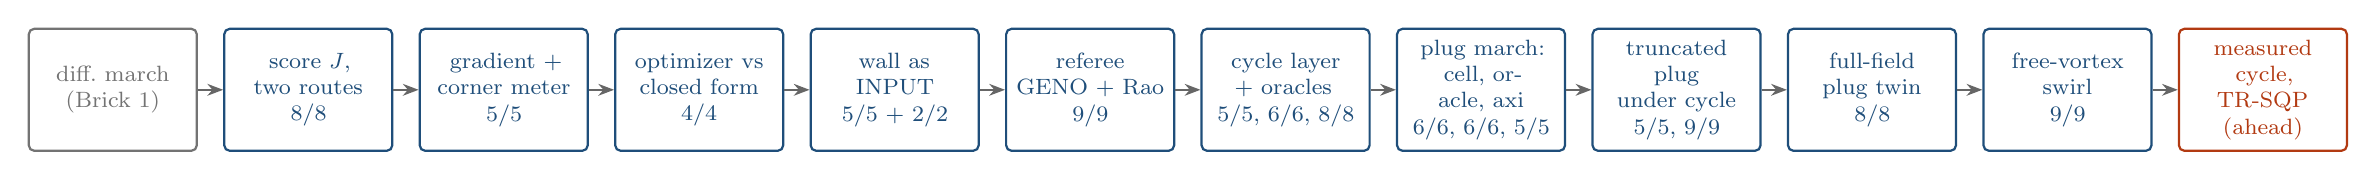
\begin{tikzpicture}[
  box/.style={draw, rounded corners=2pt, minimum height=1.55cm,
    minimum width=2.1cm, align=center, font=\footnotesize,
    text width=1.9cm, thick},
  done/.style={box, draw=stepdone, text=stepdone},
  ahead/.style={box, draw=stepahead, text=stepahead},
  arr/.style={-{Stealth[length=2mm]}, thick, color=black!60},
  node distance=0.32cm]
\node[box, draw=black!55, text=black!55] (b1)
  {diff.\ march\\(Brick 1)};
\node[done, right=of b1] (s1) {score $J$,\\two routes\\8/8};
\node[done, right=of s1] (s2) {gradient +\\corner meter\\5/5};
\node[done, right=of s2] (s3) {optimizer vs\\closed form\\4/4};
\node[done, right=of s3] (s4) {wall as\\INPUT\\5/5 + 2/2};
\node[done, right=of s4] (s5) {referee\\GENO + Rao\\9/9};
\node[done, right=of s5] (s6) {cycle layer\\+ oracles\\5/5, 6/6, 8/8};
\node[done, right=of s6] (s7) {plug march:\\cell, oracle, axi\\6/6, 6/6, 5/5};
\node[done, right=of s7] (s8) {truncated plug\\under cycle\\5/5, 9/9};
\node[done, right=of s8] (s9) {full-field\\plug twin\\8/8};
\node[done, right=of s9] (s10) {free-vortex\\swirl\\9/9};
\node[ahead, right=of s10] (s11) {measured cycle,\\TR-SQP\\(ahead)};
\draw[arr] (b1) -- (s1);
\draw[arr] (s1) -- (s2);
\draw[arr] (s2) -- (s3);
\draw[arr] (s3) -- (s4);
\draw[arr] (s4) -- (s5);
\draw[arr] (s5) -- (s6);
\draw[arr] (s6) -- (s7);
\draw[arr] (s7) -- (s8);
\draw[arr] (s8) -- (s9);
\draw[arr] (s9) -- (s10);
\draw[arr] (s10) -- (s11);
\end{tikzpicture}%
}
\caption{The Brick-2 pipeline. Each box is a chapter of this
document and carries its own certified test suite, with its pass
count shown. Blue: done and certified. Red: the road ahead. Grey:
Brick~1, the prerequisite solver.}
\label{fig:pipeline}
\end{figure}

\section{Environment and provenance}

Work of record ran on host \code{s2} in
\code{RDE\_Design-rde-nozzle-program/} (environment \code{.venv-a1}:
JAX 0.10.2, SciPy, Cantera 3.2.0, Matplotlib). This host's tree is
not a version-controlled checkout: files are ported to the
repository for commit, with a handoff note in \code{validation/}.
The referee code GENO was rebuilt from source on this host
(Chapter~\ref{ch:referee}). Every ``results of record'' block quotes
the carrier script whose output it is, and
Chapter~\ref{ch:status} lists the one-command reproduction for each.

\chapter{Che cosa fa un ugello e che cosa significa ``ottimale''}
\label{ch:nozzle}

Questo capitolo non presuppone alcuna conoscenza pregressa. Spiega
qual è la macchina in esame, a che cosa serve, quali numeri la
descrivono, perché ci sia qualcosa da ottimizzare e che cosa renda i
motori a detonazione rotante un problema di progetto più difficile
dei razzi ordinari. Chi già progetta ugelli può passare al
Capitolo~\ref{ch:moc}; tutti gli altri dovrebbero leggerlo, perché
ogni capitolo successivo usa questo vocabolario senza rispiegarlo.

\section{La macchina}

Un razzo brucia propellente in una camera, producendo gas ad alta
pressione e alta temperatura ma senza una direzione privilegiata.
L'ugello è la parte che converte quella pressione immagazzinata in
uno scarico veloce e orientato --- e, per il terzo principio di
Newton, la reazione al lancio all'indietro di quello scarico è la
spinta.

La forma che fa questo è l'ugello \emph{convergente--divergente}
della Figura~\ref{fig:nozzleprimer}a: il condotto si restringe fino
a un'area minima, la \emph{gola}, e poi torna ad allargarsi. Il
restringimento accelera il gas esattamente fino alla velocità locale
del suono in gola; oltre la gola, in flusso supersonico, il
comportamento si inverte --- allargare il condotto accelera
ulteriormente il gas. Così la parte divergente, che è ciò che questo
documento progetta, continua a convertire pressione in velocità fino
all'uscita.

Tre conseguenze contano in tutto il seguito.

\emph{La gola fissa la portata.} Quando il flusso raggiunge la
velocità del suono in gola, il condotto è \emph{bloccato}: la massa
di gas al secondo, $\dot m$, è fissata dall'area di gola e dallo
stato di camera, e nulla a valle può cambiarla. Tenere fisso il
raggio di gola $y_t$ è dunque la stessa cosa che tenere fissa la
portata --- fatto che questo documento usa come vincolo di progetto.

\emph{Lo stato di camera si esprime come stato di ristagno.} La
pressione di camera $P_0$ e la temperatura $T_0$ (i valori di
\emph{ristagno} --- ciò che il gas avrebbe se portato a riposo) sono
i dati al contorno dell'intero problema. Tutto ciò che sta a valle è
lo stesso gas, espanso.

\emph{L'uscita è un compromesso con il mondo esterno.} Il gas esce a
una certa pressione $p_e$, in un'atmosfera a pressione $p_a$. Non è
detto che siano uguali, e proprio il fatto che lo siano o no è ciò
che rende il progetto non banale.

\begin{figure}[htbp]
\centering
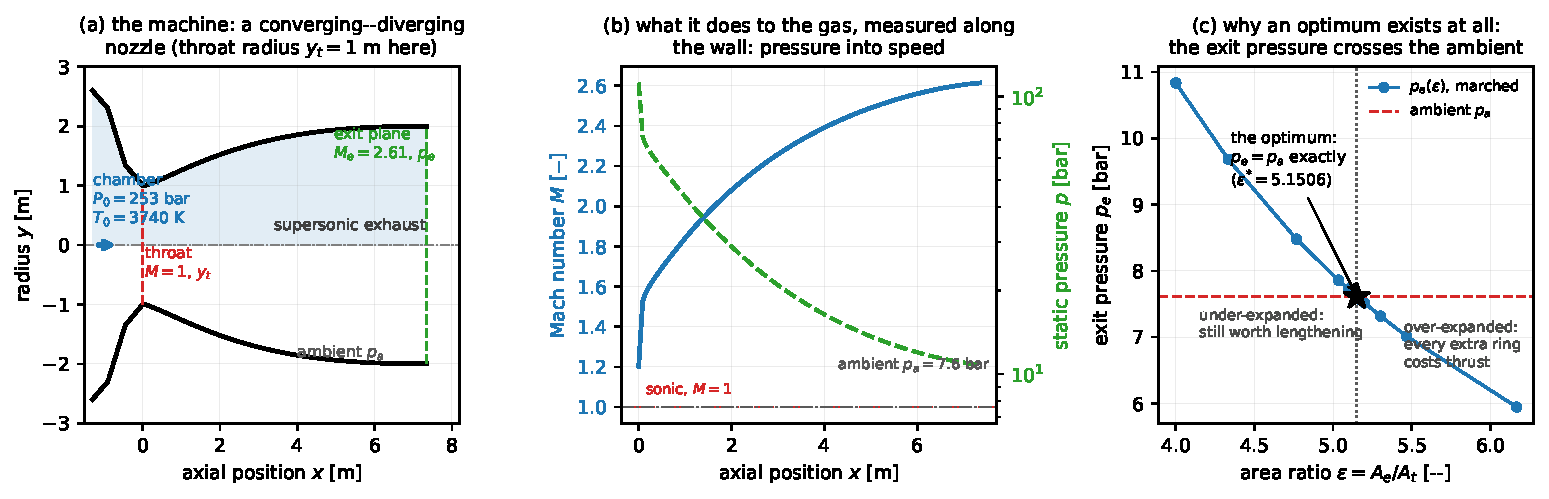
\includegraphics[width=\textwidth]{fig_nozzle_primer.pdf}
\caption{La macchina, ciò che fa e perché ha un ottimo. (a)~Un
ugello convergente--divergente: il gas dalla camera (a sinistra)
accelera fino a condizioni soniche in gola e poi supersoniche nella
parte divergente; gli assi sono posizione assiale $x$ [m] e raggio
$y$ [m], con raggio di gola $y_t = 1$~m in questo caso di
riferimento. (b)~Che cosa fa davvero l'ugello al gas, misurato con
il solutore di questo documento lungo la parete: il numero di Mach
(blu, asse sinistro, adimensionale) cresce mentre la pressione
statica (verde, asse destro, bar, logaritmica) cala di due ordini di
grandezza --- si sta scambiando pressione con velocità. (c)~Perché
esista un ottimo: la pressione di uscita $p_e$ [bar] cala al
crescere del rapporto di espansione $\varepsilon$ [--]. Sopra la
linea dell'ambiente conviene ancora allungare l'ugello; sotto, la
lunghezza in più costa spinta. La stella segna il punto in cui si
incrociano --- l'ottimo, che il Capitolo~\ref{ch:firstopt} trova
\emph{alla cieca} e verifica contro questo incrocio.}
\label{fig:nozzleprimer}
\end{figure}

\section{I numeri che descrivono un progetto}

Bastano poche grandezze per enunciare un problema di progetto, e
questo documento si attiene a quelle (l'elenco completo dei simboli
è la Tabella~\ref{tab:notation}).

Il \emph{rapporto di espansione} $\varepsilon = A_e/A_t$ --- area di
uscita diviso area di gola --- è il numero singolo più importante:
dice quanto il gas viene espanso. Un $\varepsilon$ maggiore significa
un ugello più lungo e più largo, uno scarico più veloce e più
freddo, una pressione di uscita più bassa. Il \emph{contorno di
parete} è la forma stessa, la curva $y(x)$ dalla gola all'uscita. La
\emph{lunghezza} $L$ è il punto in cui quella curva si ferma. E
$p_a$, la pressione ambiente, è l'ambiente: circa 1~bar a livello
del mare, essenzialmente nulla nel vuoto.

\section{La spinta, e perché esiste un ottimo}

La spinta è un bilancio di quantità di moto. Scritta sul piano di
uscita è
\begin{equation}
J \;=\; \dot m\,u_e \;+\; (p_e - p_a)\,A_e ,
\label{eq:thrustintro}
\end{equation}
dove il primo termine è la quantità di moto portata fuori dallo
scarico (portata per velocità di uscita) e il secondo la forza netta
di pressione sull'area di uscita. Il Capitolo~\ref{ch:score} calcola
questa quantità in due modi indipendenti come autoverifica, ma la
fisica dell'ottimo è già visibile nella~\eqref{eq:thrustintro}.

Si supponga di allungare leggermente l'ugello, aggiungendo un
sottile anello di parete. Il gas interno spinge su quell'anello con
pressione $p$; l'atmosfera spinge in senso opposto con $p_a$. Il
guadagno netto è proporzionale a $p - p_a$. Dunque, finché lo
scarico è a pressione maggiore dell'ambiente --- il flusso è
\emph{sotto-espanso} --- la lunghezza in più paga. Una volta che il
flusso si è espanso oltre l'ambiente --- \emph{sovra-espanso} ---
ogni anello aggiuntivo spinge dalla parte sbagliata e costa spinta.
Il progetto migliore sta esattamente al cambio di segno:
\begin{equation}
p_e(\varepsilon^{*}) \;=\; p_a .
\label{eq:matchintro}
\end{equation}
La Figura~\ref{fig:nozzleprimer}c è quell'affermazione, misurata.
Questa singola idea --- estendere la parete finché la pressione
locale supera l'ambiente, fermarsi quando non lo fa --- ricompare in
tutto il documento in forma via via più generale: come condizione
terminale al labbro dell'ugello (Capitolo~\ref{ch:score}), come
condizione mediata su un ciclo (Capitolo~\ref{ch:cycle}) e come
regola che decide dove troncare un ugello a spina
(Capitolo~\ref{ch:plugcycle}).

Un caso particolare importante: nel vuoto $p_a = 0$, quindi
$p - p_a$ è positivo ovunque e \emph{più lungo è sempre meglio}. Non
esiste un ottimo interno, solo la lunghezza che il veicolo riesce a
portare. Qualunque ottimizzatore degno di fiducia deve riprodurre
quel comportamento, e diversi test di questo documento verificano
esattamente questo.

\section{Tre famiglie di ugello, e perché la terza è difficile}

\emph{L'ugello ideale (a lunghezza minima)} è la forma da manuale:
il suo contorno è tracciato in modo che lo scarico esca
perfettamente uniforme e parallelo. È facile da caratterizzare e qui
serve da riferimento; lo genera il Mattone~1.

\emph{Il contorno ottimizzato in spinta}, secondo la soluzione di
Rao del 1958~\cite{rao}, rinuncia all'uscita perfettamente uniforme
e pone una domanda migliore: fra tutte le pareti di una \emph{data
lunghezza}, quale produce la massima spinta? La risposta è una forma
più corta e più piena, ed è quella che i razzi reali usano. Rao la
risolse con il calcolo delle variazioni --- la matematica
dell'ottimizzazione su un'intera curva anziché su pochi numeri --- e
il Capitolo~\ref{ch:referee} confronta le sue condizioni derivate a
mano con la macchina automatica di questo programma proprio su un
contorno di quel tipo.

\emph{L'ugello a spina (o aerospike)} rovescia la geometria
(Figura~\ref{fig:bellvsplug}). Invece che il gas sia racchiuso da
una parete, la superficie solida --- la \emph{spina} --- sta sotto,
e la frontiera esterna dello scarico non è altro che l'atmosfera
circostante. Quella frontiera libera è ciò che rende interessante il
plug: non è fissata dall'hardware, quindi il pennacchio si
riconfigura quando la pressione ambiente cambia. Una campana è
ottimale a una quota; un plug è all'incirca giusto su un
intervallo, perché lo scarico finisce sempre esattamente a $p_a$ sul
suo bordo esterno, per definizione. La
Figura~\ref{fig:bellvsplug}c mostra questo, calcolato. I plug reali
sono sempre \emph{troncati} --- tagliati corti e chiusi con una base
piatta --- perché la coda lunga e sottile porta quasi nessuna
pressione ma tutto il peso, e dove tagliare è una genuina variabile
di progetto (Capitolo~\ref{ch:plugcycle}).

\begin{figure}[htbp]
\centering
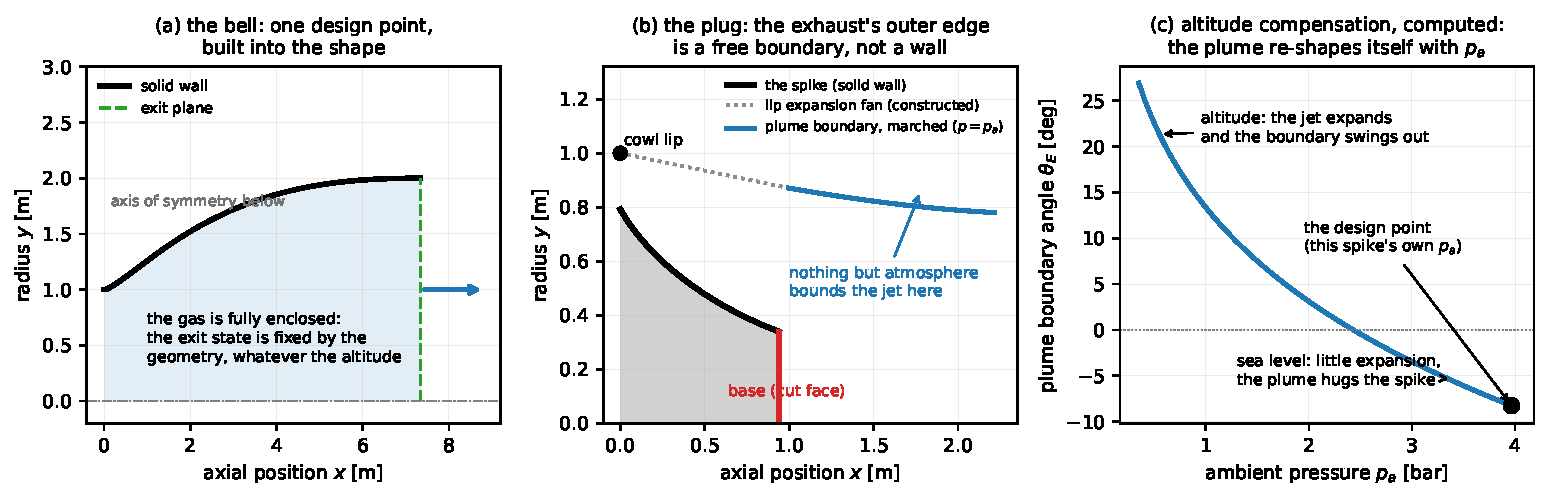
\includegraphics[width=\textwidth]{fig_bell_vs_plug.pdf}
\caption{Le due famiglie di ugello che questo documento costruisce e
l'unica differenza fisica fra loro. Gli assi sono ovunque posizione
assiale $x$ [m] e raggio $y$ [m]. (a)~La campana: lo scarico è
racchiuso da una parete solida, quindi lo stato di uscita è fissato
dalla geometria, qualunque sia la quota. (b)~Il plug (aerospike): la
spina solida sta sotto e il bordo esterno del getto è una
\emph{frontiera libera} a pressione ambiente. La spina mostrata è un
contorno realmente progettato (dal codice indipendente del
Capitolo~\ref{ch:genotwin}); la frontiera del pennacchio è calcolata
dalla marcia del Capitolo~\ref{ch:plug}; la faccia rossa è la base
dove la spina viene troncata. (c)~Compensazione di quota, calcolata
sullo stesso gas: l'angolo della frontiera del pennacchio $\theta_E$
[gradi] in funzione della pressione ambiente $p_a$ [bar]. Ad
ambiente alto il getto si espande appena e resta aderente alla
spina; al calare dell'ambiente la frontiera ruota verso l'esterno
--- l'ugello che si adatta, senza parti in movimento.}
\label{fig:bellvsplug}
\end{figure}

\section{Il motore a detonazione rotante, e il ciclo}
\label{sec:rdeintro}

Tutto quanto sopra assumeva un solo punto di funzionamento: una
pressione di camera, un ambiente. Un \emph{motore a detonazione
rotante} (RDE) infrange quell'assunzione, ed è la ragione per cui
questo documento ha uno strato di ciclo.

In un RDE la combustione non sta ferma a bruciare in modo stazionario.
Una detonazione --- un'onda di combustione che viaggia più veloce
del suono --- corre di continuo \emph{attorno} a una camera anulare,
percorrendola qualche migliaio di volte al secondo
(Figura~\ref{fig:rdecycle}a). Il propellente fresco viene iniettato
dietro l'onda e consumato al giro successivo. L'attrattiva è
termodinamica: la combustione detonativa alza la pressione mentre
brucia, quindi un RDE promette più lavoro dallo stesso propellente
rispetto a una combustione stazionaria.

La conseguenza per l'ugello è severa. Una sezione fissa dello
scarico non vede uno stato di camera costante; vede il picco di
pressione al passaggio dell'onda e poi il decadimento fino al giro
successivo --- ancora e ancora, migliaia di volte al secondo. Ciò
che viene consegnato all'ugello non è dunque un solo stato di
ristagno ma una \emph{famiglia periodica} di stati,
$(P_0(\xi), T_0(\xi))$, etichettati dalla posizione nel ciclo, la
\emph{fase} $\xi \in [0,1]$ (Figura~\ref{fig:rdecycle}b).

Poiché il gas attraversa l'ugello molto più in fretta di quanto
cambino le condizioni di camera, ogni fase può essere trattata come
un proprio flusso stazionario, e la prestazione dell'intero ciclo è
la media delle prestazioni stazionarie sulle fasi. Quell'ipotesi si
chiama \emph{quasi-stazionaria}; è ciò che rende il problema
trattabile con la macchina di questo documento, è dichiarata
esplicitamente ovunque venga usata, e i suoi limiti sono discussi
onestamente nella Sezione~\ref{sec:spiral}.

La difficoltà di progetto è allora immediata ed è l'intero soggetto
dei Capitoli~\ref{ch:cycle} e~\ref{ch:plugcycle}: ogni fase
vorrebbe un ugello diverso (Figura~\ref{fig:rdecycle}c), e di
hardware se ne costruisce uno solo. Qual è il compromesso giusto ---
ed è semplicemente l'ugello per la condizione media di camera? Per
un tipo di ugello la risposta risulta essere sì, esattamente; per un
altro è decisamente no. Misurare entrambi è ciò che questo documento
fa.

\begin{figure}[htbp]
\centering
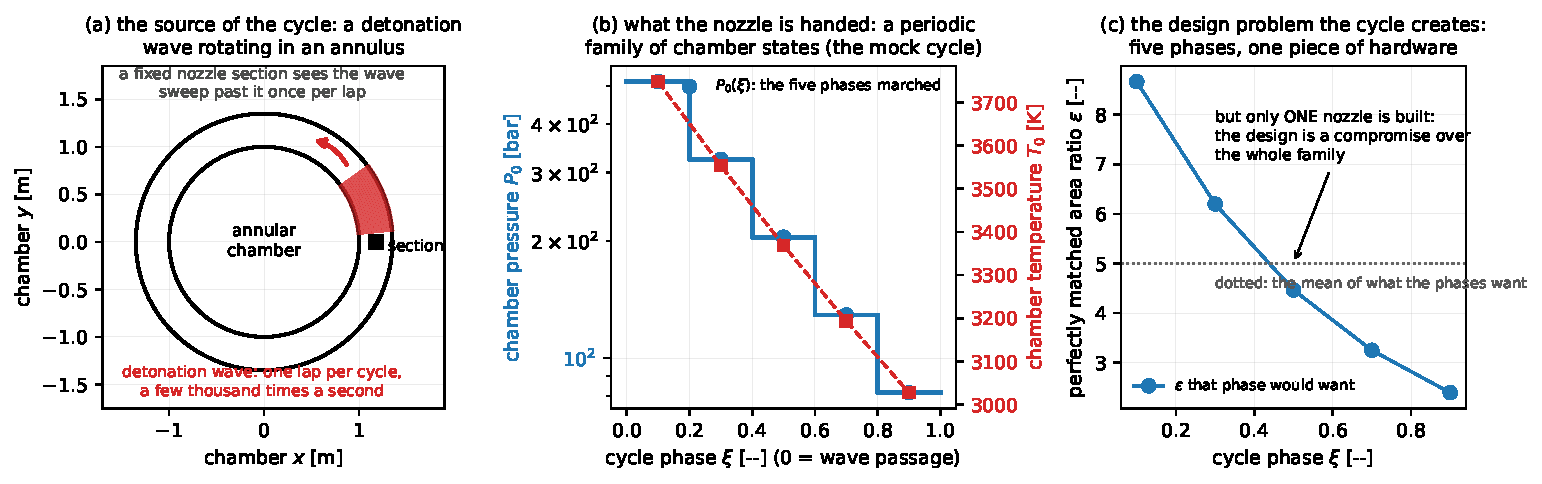
\includegraphics[width=\textwidth]{fig_rde_cycle.pdf}
\caption{Perché l'ugello di un RDE è un problema di progetto più
difficile. (a)~L'origine del ciclo: un'onda di detonazione corre
attorno a una camera anulare (gli assi sono coordinate della sezione
di camera $x, y$ [m]); una sezione fissa di ugello la vede passare
una volta per giro, qualche migliaio di volte al secondo. (b)~Ciò
che viene quindi consegnato all'ugello: non un punto di
funzionamento ma una famiglia periodica. Fase di ciclo $\xi$ [--]
sull'asse orizzontale ($\xi = 0$ al passaggio dell'onda), pressione
di camera $P_0$ [bar] sull'asse sinistro (logaritmico, blu) e
temperatura di camera $T_0$ [K] su quello destro (rosso) --- le
cinque fasi discrete effettivamente marciate dai carrier. (c)~Il
problema di progetto che ne risulta: per ogni fase, il rapporto di
espansione $\varepsilon$ [--] che sarebbe perfettamente adattato per
\emph{quella} fase, calcolato con le tabelle di gas del programma.
Si distribuiscono su un fattore tre, e di ugello se ne costruisce
uno solo.}
\label{fig:rdecycle}
\end{figure}

\section{Che cosa significa qui ``ottimizzare'', e che cosa dà un
aggiunto}

Un \emph{ottimizzatore} ha bisogno di tre cose che un solutore di
flusso non possiede. Un \emph{punteggio}: un numero che dica quanto
è buono un progetto --- qui la spinta $J$, costruita nel
Capitolo~\ref{ch:score}. Una \emph{bussola}: la derivata di quel
punteggio rispetto a ogni variabile di progetto, il
\emph{gradiente}, che dice in che direzione muoversi. E un
\emph{certificato}: una condizione che riconosca un ottimo quando lo
si raggiunge, così che ``la ricerca si è fermata'' e ``il progetto è
ottimale'' siano affermazioni distinte.

Il gradiente è il punto in cui la tecnologia del Mattone~1 conta. Se
un progetto ha una sola manopola, il gradiente si può stimare per
\emph{differenze finite} --- si cambia un poco la manopola e si
guarda come cambia $J$. Con un'intera forma di parete come incognita
questo costa una soluzione di flusso in più per ogni grado di
libertà, il che è senza speranza. La \emph{differenziazione
automatica} (AD) evita tutto ciò. Poiché il solutore è scritto in un
linguaggio che registra l'aritmetica che esegue, la regola della
catena può essere applicata all'indietro attraverso l'intero calcolo,
producendo la derivata di $J$ rispetto a \emph{tutti} gli ingressi
in una volta sola, al costo di circa una risoluzione aggiuntiva e
con accuratezza di macchina anziché con quella di un rapporto
incrementale. Questa passata all'indietro è matematicamente lo
stesso oggetto dell'\emph{aggiunto discreto} della teoria classica
del controllo ottimo --- da cui il nome di questo pacchetto di
lavoro --- ma si ottiene gratis anziché derivarlo e programmarlo a
mano.

Questo è il motore. Il resto del documento gli costruisce attorno un
ottimizzatore, un pezzo certificato alla volta.

\chapter{Come calcola il solutore}
\label{ch:moc}

Il resto di questo documento parla di continuo di ``celle'',
``colonne'', ``piedi'', ``caratteristiche'' e ``compatibilità''.
Questo capitolo le definisce tutte partendo da zero. Descrive il
\emph{metodo delle caratteristiche}, il metodo numerico su cui posa
l'intero programma, e vale le quattro pagine che occupa: quasi ogni
lezione tecnica registrata più avanti --- compreso ogni difetto in
appendice --- è un'affermazione sugli oggetti qui introdotti.

\section{L'unico fatto fisico che il metodo sfrutta}

In un gas che si muove \emph{più lentamente} del suono, una
perturbazione si propaga in ogni direzione, a monte compreso:
l'intero campo di moto è accoppiato a sé stesso, e risolverlo
significa risolvere ovunque simultaneamente. In un gas che si muove
\emph{più velocemente} del suono, questo non può avvenire. Una
perturbazione prodotta in un punto viene trascinata a valle più in
fretta di quanto riesca a propagarsi, quindi la sua influenza è
confinata a un cuneo che si apre a valle di quel punto.

Quel cuneo ha un semiangolo preciso, l'\emph{angolo di Mach}
$\alpha$, dato da
\begin{equation}
\sin\alpha = \frac{1}{M}, \qquad M = \frac{q}{c},
\label{eq:machangle}
\end{equation}
dove $q$ è la velocità del flusso, $c$ la velocità locale del suono
e $M$ il loro rapporto, il \emph{numero di Mach}. Un flusso più
veloce dà un cuneo più stretto. I suoi due lati, tracciati per il
punto, sono le \emph{caratteristiche}: uno a un angolo
$\theta + \alpha$ rispetto all'asse e uno a $\theta - \alpha$, dove
$\theta$ è la direzione in cui il gas sta effettivamente scorrendo
(Figura~\ref{fig:mocprimer}a). Per convenzione la prima famiglia si
chiama $C^{+}$ e la seconda $C^{-}$.

Le caratteristiche non sono solo geometria. Lungo ciascuna di esse
il flusso deve soddisfare una \emph{relazione di compatibilità}:
un'equazione differenziale ordinaria che lega la variazione di
velocità alla variazione di direzione del flusso, con un termine
aggiuntivo nel flusso assialsimmetrico che tiene conto del condotto
che si allarga al crescere del raggio. Questo è l'intero contenuto
fisico che il solutore usa. Due famiglie di linee, una relazione
lungo ciascuna --- nessuna griglia di volume, nessun avanzamento nel
tempo, nessuna iterazione fino allo stato stazionario.

\section{Il processo elementare: una cella}

Il metodo trasforma quelle relazioni in aritmetica con una singola
mossa ripetuta, la \emph{cella} (o \emph{processo elementare}),
mostrata in Figura~\ref{fig:mocprimer}b.

Si supponga che due punti vicini siano già risolti: posizione e
velocità note in entrambi. Dal punto inferiore si traccia la sua
caratteristica $C^{+}$; da quello superiore la sua $C^{-}$. In
flusso supersonico queste due linee convergono e si incrociano in
esattamente un punto a valle. Quell'incrocio fornisce due equazioni,
una per linea, per le due coordinate del nuovo punto. Le due
relazioni di compatibilità, integrate lungo i due brevi segmenti
appena tracciati, danno altre due equazioni per le due componenti di
velocità lì. Quattro equazioni, quattro incognite $(x, y, u, v)$.

Le equazioni sono non lineari --- le direzioni caratteristiche
dipendono proprio dallo stato che si sta cercando --- quindi ogni
cella è chiusa da una piccola iterazione di Newton. Due dettagli su
come vengono chiuse contano più avanti:

\emph{Coefficienti al punto medio.} I coefficienti delle relazioni
di compatibilità sono valutati non all'inizio del segmento ma nel
suo \emph{punto medio}, usando la media dei due stati agli estremi.
È la regola dei trapezi; fa sì che l'errore per cella si riduca con
il quadrato del passo anziché linearmente, ed è il motivo per cui
l'intera marcia si dice del secondo ordine. È anche la ragione per
cui una cella non deve mai attraversare una regione in cui lo stato
cambia bruscamente: mediare i due estremi di un tale segmento è
allora privo di significato (il Capitolo~\ref{ch:plug} contiene un
esempio misurato).

\emph{Certificazione di Newton.} Una volta che l'iterazione di
Newton di una cella è convergita, il programma verifica che il
residuo delle quattro equazioni sia davvero sceso al livello
dell'arrotondamento in virgola mobile, scalato con la dimensione
delle incognite. Una cella che si arena viene colta e segnalata
invece di inquinare in silenzio la marcia. Ogni affermazione
``tutte le celle certificate da Newton'' in questo documento è
quella verifica, eseguita su ogni cella.

\section{Colonne, frontiere e piedi}

I nuovi punti crescono da punti risolti, quindi una marcia si
organizza in \emph{colonne}: da una colonna risolta, le celle
interne producono la colonna successiva, e la spazzata si ripete
verso valle (Figura~\ref{fig:mocprimer}c). Una marcia ha dunque
bisogno di un punto da cui cominciare --- una \emph{linea iniziale}
(o linea dei valori iniziali) attraverso il flusso, sulla quale lo
stato completo è fornito come dato. In un ugello di razzo quella
linea sta appena a valle della gola.

Ai bordi del flusso la cella cambia forma, perché una delle sue due
caratteristiche genitrici manca e una condizione al contorno ne
prende il posto. In questo documento compaiono tre frontiere.

\emph{Un asse di simmetria}: il flusso non può attraversarlo, il che
fornisce la relazione mancante.

\emph{Una parete assegnata}: la posizione del nuovo punto è già
nota, perché deve trovarsi su un contorno dato con una pendenza
data. La cella allora lavora \emph{all'indietro}. Deve trovare il
\emph{piede} --- il punto sulla colonna precedente da cui la
caratteristica in arrivo è partita --- che in generale cade fra due
punti memorizzati e va localizzato cercando lungo la colonna e
interpolando. La relazione di compatibilità viene poi chiusa lungo
la corda da quel piede al punto di parete. È questa la cella che
permette a un progettista di consegnare una parete arbitraria
(Capitolo~\ref{ch:wallinput}), e l'accuratezza della ricerca del
piede è un tema ricorrente.

\emph{Una frontiera di getto libero}: il caso in cui non c'è parete
alcuna e lo scarico è delimitato dall'atmosfera. Qui la situazione è
esattamente rovesciata: la \emph{pressione} è nota (è $p_a$, poiché
sul getto non spinge altro che l'atmosfera) mentre la
\emph{posizione} della frontiera è incognita e va risolta. È questo
l'unico pezzo di fisica genuinamente nuovo di cui l'ugello a spina
ha bisogno, e il Capitolo~\ref{ch:plug} lo costruisce e lo
certifica.

\begin{figure}[htbp]
\centering
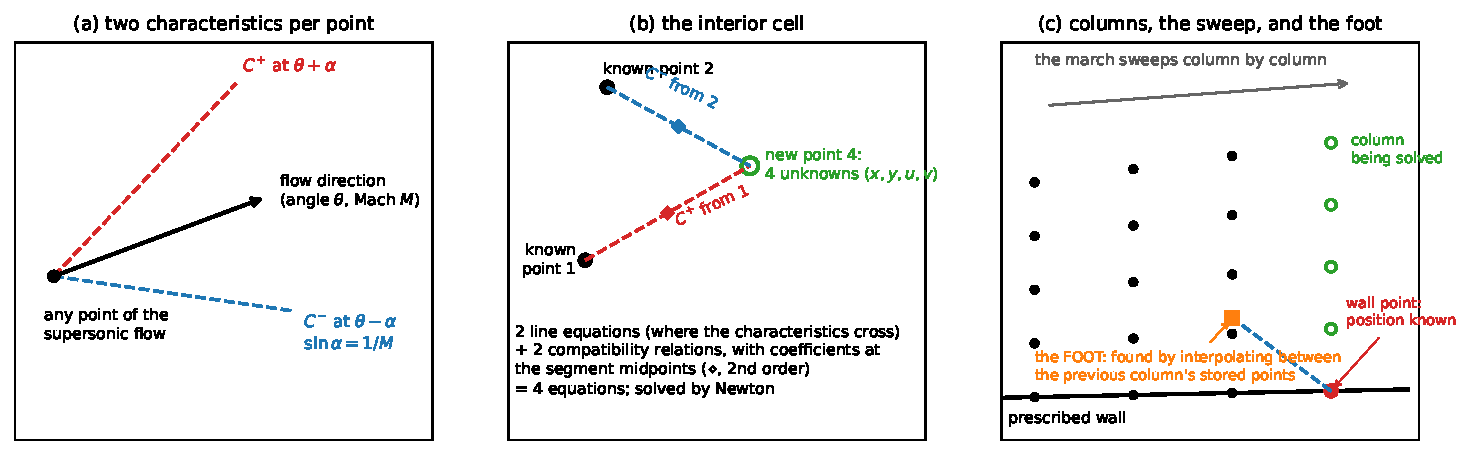
\includegraphics[width=\textwidth]{fig_moc_primer.pdf}
\caption{Come calcola la marcia, per un lettore nuovo al metodo
delle caratteristiche. Gli assi sono ovunque posizione assiale $x$
[m] e raggio $y$ [m]. (a)~Per ogni punto di un flusso supersonico
passano due caratteristiche, inclinate dell'angolo di Mach $\alpha$
da una parte e dall'altra della direzione locale del flusso
$\theta$; lungo ciascuna, una relazione di compatibilità lega la
variazione di velocità alla variazione di angolo. (b)~La cella
interna: da due punti già risolti, l'incrocio di una $C^{+}$ e di
una $C^{-}$ fissa la posizione del nuovo punto, e le due relazioni
di compatibilità --- chiuse con coefficienti presi nei punti medi
dei segmenti ($\diamond$) --- ne fissano la velocità; un'iterazione
di Newton risolve il sistema $4\times4$ che ne risulta. (c)~Le celle
costruiscono colonne a partire da colonne. A una parete assegnata la
posizione è nota anziché calcolata, quindi la cella deve localizzare
per interpolazione il \emph{piede} della caratteristica in arrivo
sulla colonna precedente. Ogni lezione strutturale del
Capitolo~\ref{ch:plug} e dell'Appendice~\ref{ch:appendix} è
un'affermazione su queste tre figure.}
\label{fig:mocprimer}
\end{figure}

\section{Spigoli vivi: l'unica cosa che una cella non sa fare}

Dove una parete gira uno spigolo vivo, il flusso si espande
attraverso un \emph{ventaglio di espansione centrato}: una
distribuzione continua di caratteristiche tutte uscenti da quel
singolo punto geometrico, ciascuna portatrice di uno stato diverso.
Nello spigolo stesso il flusso è dunque a più valori e i gradienti
sono infiniti.

Nessuna cella ordinaria può scavalcare un tale ventaglio, per
entrambe le ragioni dette sopra: un segmento che attraversasse il
ventaglio medierebbe stati che differiscono per l'intera rotazione,
e vicino allo spigolo l'incrocio di caratteristiche che fissa la
nuova posizione degenera perché tutte le linee si incontrano in un
punto solo. Il rimedio è che un ventaglio centrato non ha bisogno di
essere marciato --- è \emph{autosimile}, quindi lo stato su ogni
raggio è noto in forma chiusa a partire dal solo angolo del raggio.
Lo spigolo viene perciò \emph{costruito} come dato e le celle
ordinarie riprendono fra i raggi, dove il flusso è di nuovo
regolare. Il Capitolo~\ref{ch:plug} mostra che cosa accade quando
questa regola viene violata, con il numero misurato.

\section{Gas reale, e da dove vengono le derivate}

Vale la pena enunciare qui, una volta per tutte, due scelte
implementative.

Il gas non è assunto caloricamente perfetto. Le proprietà
termodinamiche provengono da dati tabulati, e lo stato è recuperato
dalla velocità attraverso le relazioni di energia ed entropia.
Questo conta in un modo non ovvio che il
Capitolo~\ref{ch:wallinput} documenta: le proprietà tabulate sono
interpolate a tratti, quindi la derivata \emph{esatta} del codice
porta una piccola increspatura alla scala delle celle della tabella
--- una proprietà reale dell'obiettivo discreto, non un difetto, ma
tale da rendere mal posto un ingenuo test sulle derivate.

E l'intera marcia --- ogni cella, ogni iterazione di Newton, ogni
ricerca del piede --- è scritta in modo da poter essere
differenziata automaticamente. È questo che trasforma un solutore
nel motore di un ottimizzatore, ed è il soggetto di tutto ciò che
segue.

\chapter{Come questo programma decide che qualcosa è vero}
\label{ch:method}

Un codice di progetto vale quanto le prove che è corretto. Questo
capitolo enuncia le due regole cui ogni suite di test del documento
obbedisce, spiega perché sono state scelte e definisce i pochi
termini usati per riportare i risultati. Si chiude con la tabella
dei simboli valida per l'intero documento.

\section{Regola uno: nessuna tolleranza è scelta a mano}

Ogni verifica di questo documento confronta un numero calcolato con
una banda, e \emph{nessuna banda è scelta da un essere umano}. La
ragione è semplice: una tolleranza scelta dopo aver visto la
risposta non certifica nulla. Esiste sempre, e passa sempre.

La banda è invece \emph{derivata}, e in quasi tutti i casi è il
calcolo stesso a derivarla su di sé. La stessa quantità viene
calcolata due volte, una su una discretizzazione grossolana e una su
una fine. La differenza fra le due è una misura dell'errore che lo
schema sta ancora commettendo. La banda è quella differenza,
moltiplicata per un fattore di sicurezza fisso
$K_{\rm RICH} = 4$, più un pavimento al livello
dell'arrotondamento in virgola mobile:
\begin{equation}
\text{banda} \;=\; K_{\rm RICH}\,
\bigl|\,\text{grossolana} - \text{fine}\,\bigr|
\;+\; \text{pavimento di arrotondamento}.
\label{eq:band}
\end{equation}
È la classica idea dell'\emph{estrapolazione di Richardson} usata
come stima dell'errore anziché come acceleratore, e il numero che ne
risulta è chiamato ovunque \emph{banda di Richardson}
(Figura~\ref{fig:method}b). Poiché il metodo è del secondo ordine
(Capitolo~\ref{ch:moc}), dimezzare il passo dovrebbe ridurre
l'errore di circa quattro volte; quando una suite riporta un
``rapporto grossolana/fine di 4.52'' sta riportando che lo schema
converge al ritmo che dovrebbe, il che è già di per sé una prova
che la banda significa qualcosa.

Non tutte le quantità hanno una discretizzazione da raffinare. Dove
non c'è, la banda è derivata da qualcos'altro di misurabile --- la
dispersione dei dati di riferimento stessi, o la scala fisica della
quantità --- e la fonte è sempre dichiarata. Un capitolo (il
Capitolo~\ref{ch:genotwin}) usa soglie \emph{dichiarate} anziché
derivate; lo dice esplicitamente, ne dà la provenienza e spiega
perché il raffinamento sarebbe lì il metro sbagliato. Quell'eccezione
è deliberata e visibile, che è appunto il punto.

\section{Regola due: ogni suite deve saper dire di no}

Un test che non ha mai fallito potrebbe non misurare nulla. Perciò,
accanto alle verifiche positive, ogni suite contiene corruzioni
deliberate --- chiamate \emph{rigettatori} --- che la suite è tenuta
a cogliere: un segno invertito, un termine eliminato, una pressione
ambiente sbagliata, un piede caratteristico sbagliato, una geometria
perturbata di una frazione di percento. Se un rigettatore \emph{non}
fallisce, la verifica positiva corrispondente non vale nulla e il
passo non conta come fatto.

I rigettatori fanno lavoro reale in questo documento. Sono ciò che
rende affidabile una soglia dichiarata (mostrano che lo strumento
risolve difetti di un ordine di grandezza superiori al divario che
si sta misurando), e parecchi di essi hanno colto errori genuini nel
programma prima che potessero raggiungere un risultato.

La Figura~\ref{fig:method}a mette entrambe le regole in un'unica
immagine: ogni verifica del documento, espressa come deviazione
misurata divisa per la propria banda, insieme a ogni corruzione
deliberata. Le verifiche positive devono cadere a sinistra di uno; i
rigettatori devono cadere a destra. Nulla è vicino alla linea per
caso.

\begin{figure}[htbp]
\centering
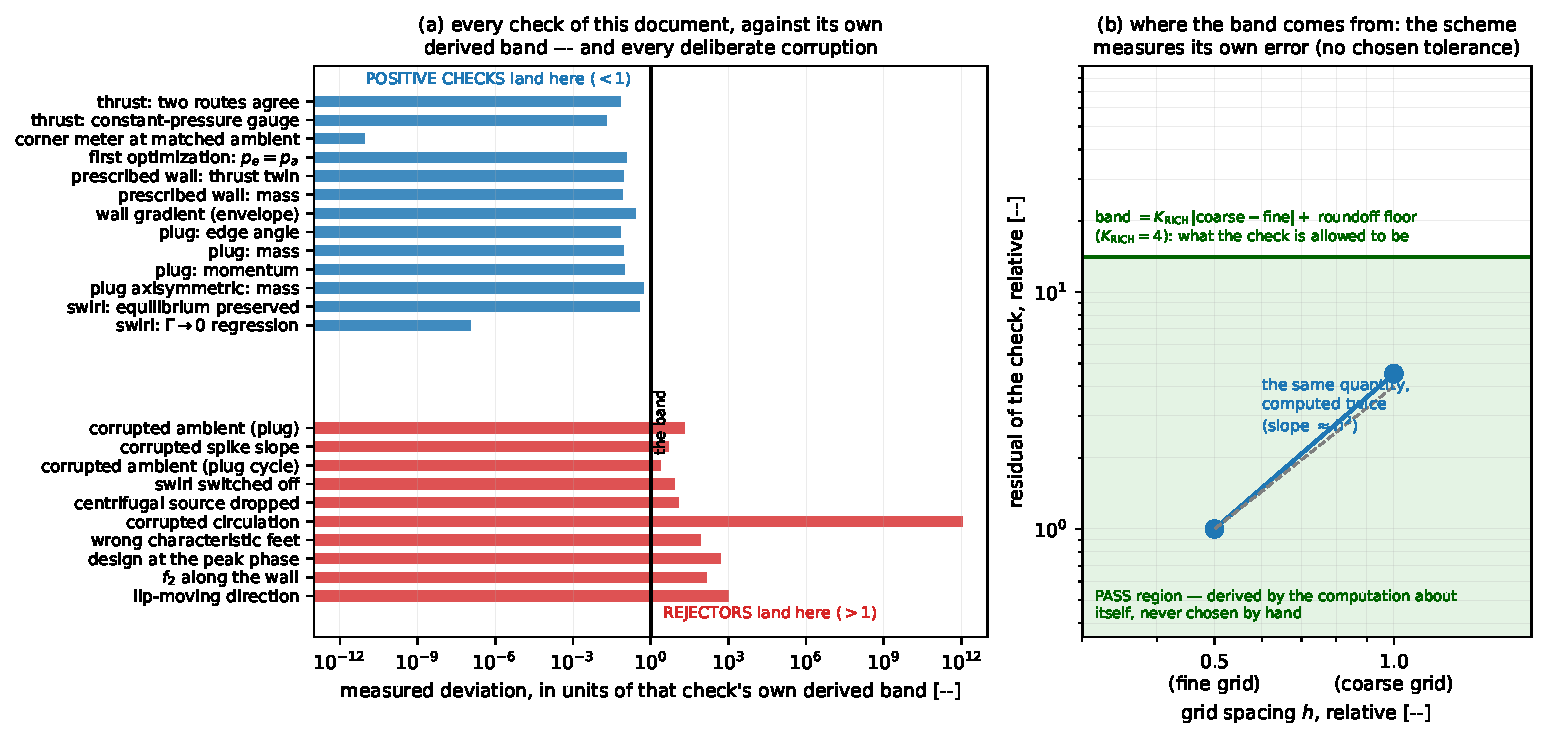
\includegraphics[width=\textwidth]{fig_method.pdf}
\caption{Il metodo di questo documento, in un'immagine. (a)~Ogni
verifica certificata (blu) e ogni corruzione deliberata (rosso),
riportate come deviazione misurata divisa per la banda derivata
\emph{propria} di quella verifica --- così l'asse orizzontale è
adimensionale e la linea verticale a uno è la soglia di
superamento/fallimento per tutte in una volta. Le verifiche positive
cadono molto a sinistra (la maggior parte da due a sei ordini di
grandezza); i rigettatori cadono molto a destra. (b)~Da dove viene
una banda: la stessa quantità è calcolata su una griglia grossolana
e su una fine, la differenza misura l'errore che lo schema sta
ancora commettendo, e la banda è quella differenza per un fattore di
sicurezza quattro più un pavimento di arrotondamento. Gli assi sono
la spaziatura di griglia $h$ e il residuo della verifica, entrambi
relativi e logaritmici; la linea tratteggiata è la pendenza del
secondo ordine che il metodo dovrebbe seguire.}
\label{fig:method}
\end{figure}

\section{Come vengono riportati i risultati}

Ricorrono alcune convenzioni.

\emph{``$m/n$ PASS''} conta le verifiche di una suite, rigettatori
compresi: una suite con sei verifiche positive e due corruzioni che
si comporta correttamente riporta 8/8.

\emph{``Certificato da Newton''} significa che il residuo convergente
di ogni cella è stato verificato essere al livello
dell'arrotondamento, scalato con la dimensione delle sue incognite
(Capitolo~\ref{ch:moc}). Il numero citato (``residuo peggiore
0.019'') è una frazione della tolleranza ammessa, quindi qualunque
valore sotto uno passa.

\emph{``Risultato di riferimento''} significa che il numero è citato
alla lettera da un'esecuzione reale del carrier nominato, non
ricalcolato per il documento. Il Capitolo~\ref{ch:status} elenca
l'unico comando che riproduce ciascuno.

\emph{Un oracolo} è un caso la cui risposta è nota indipendentemente
dal programma --- una soluzione in forma chiusa, un'identità esatta
di conservazione o un secondo codice --- rispetto al quale il
programma può essere giudicato. Dove non esiste un oracolo, una
suite ripiega sulle \emph{chiusure interne}: affermazioni di
conservazione (massa, quantità di moto) che devono valere qualunque
sia la risposta, più i \emph{controlli di vitalità}, che verificano
che un termine che il programma dichiara di includere cambi
effettivamente la risposta quando viene rimosso.

Infine, e deliberatamente: \textbf{in questo programma anche i
difetti colti dai test sono risultati.} I capitoli principali
descrivono ciascun passo così come funziona oggi; ogni trappola,
ogni svolta sbagliata e ogni lezione strutturale misurata è raccolta
nell'Appendice~\ref{ch:appendix}, con riferimenti incrociati dal
passo cui appartiene. Un difetto colto è la prova che lo strumento
ha i denti.

\section{Simboli usati nel documento}

\begin{table}[htbp]
\centering
\small
\begin{tabular}{@{}llp{7.4cm}@{}}
\toprule
Simbolo & Unità & Significato \\
\midrule
\multicolumn{3}{@{}l}{\emph{Geometria e flusso}}\\
$x$, $y$ & m & posizione assiale, raggio \\
$u$, $v$ & m/s & componenti assiale e radiale della velocità \\
$q$ & m/s & modulo della velocità, $\sqrt{u^2+v^2}$ (indicato $W$
  negli articoli di Rao) \\
$\theta$ & rad, gradi & direzione del flusso, $\arctan(v/u)$ \\
$p$, $\rho$, $T$ & Pa, kg/m$^3$, K & pressione statica, densità,
  temperatura \\
$c$ & m/s & velocità locale del suono \\
$M$ & -- & numero di Mach, $q/c$ \\
$\alpha$ & rad & angolo di Mach, $\sin\alpha = 1/M$ \\
$C^{+}$, $C^{-}$ & -- & le due famiglie caratteristiche, a
  $\theta+\alpha$ e $\theta-\alpha$ \\
$\nu(M)$ & rad & funzione di Prandtl--Meyer (la rotazione prodotta
  da un'espansione di spigolo) \\
$\delta$ & -- & 0 per flusso piano, 1 per assialsimmetrico \\
\midrule
\multicolumn{3}{@{}l}{\emph{La macchina e il suo punto di
  funzionamento}}\\
$y_t$ & m & raggio di gola (tenerlo fisso fissa la portata) \\
$r_{tu}$, $r_{td}$ & m & raggi di raccordo in gola, a monte e a
  valle \\
$A_t$, $A_e$ & m$^2$ & area di gola e di uscita \\
$\varepsilon$ & -- & rapporto di espansione, $A_e/A_t$ \\
$L$ & m & lunghezza della parete \\
$P_0$, $T_0$ & Pa, K & pressione e temperatura di camera (di
  ristagno) \\
$p_a$ & Pa & pressione ambiente (di contropressione) \\
$p_e$, $u_e$ & Pa, m/s & pressione e velocità di uscita \\
$\dot m$ & kg/s & portata \\
$J$, $F$ & N & spinta (l'obiettivo da ottimizzare) \\
\midrule
\multicolumn{3}{@{}l}{\emph{Il ciclo (motore a detonazione
  rotante)}}\\
$\xi$ & -- & fase del ciclo, $0$ al passaggio dell'onda e $1$ alla
  fine dello svuotamento \\
$\mu$ & -- & la misura che pesa le fasi nella media di ciclo \\
$PR$, $TR$ & -- & rapporto di pressione e di temperatura sul
  ciclo \\
\midrule
\multicolumn{3}{@{}l}{\emph{Ugello a spina e swirl}}\\
$l$ & m & lunghezza di troncamento: dove la spina viene tagliata \\
$D$ & -- & il punto di troncamento stesso \\
$w$ & m/s & velocità azimutale (di swirl) \\
$\Gamma$ & m$^2$/s & circolazione, $y\,w$; costante in un vortice
  libero \\
\midrule
\multicolumn{3}{@{}l}{\emph{Strumenti}}\\
$R_{\rm mom}$ & N & disaccordo fra le due vie indipendenti di
  calcolo della spinta \\
$R_{\rm corner}$ & Pa & residuo terminale (di spigolo): nullo a un
  labbro ottimale \\
$f_2$ & m/s & primo integrale di Rao,
  $q\cos(\theta-\alpha)/\cos\alpha$, costante lungo la
  caratteristica terminale di un ugello ottimale \\
$\lambda_2$, $\lambda_3$ & -- & moltiplicatori di Lagrange costanti
  di Rao ($f_2 = -\lambda_2$) \\
$K_{\rm RICH}$ & -- & fattore di sicurezza di Richardson, fissato
  a 4 \\
\bottomrule
\end{tabular}
\caption{Simboli usati in tutto questo documento. Le lunghezze sono
espresse in metri; i casi di riferimento sono posti con raggio di
gola $y_t = 1$~m, quindi i valori numerici di $x$ e $y$ sono anche
multipli del raggio di gola.}
\label{tab:notation}
\end{table}

\chapter{Il punteggio e la bussola}
\label{ch:score}

Il solutore del Mattone~1 risponde alla domanda ``che cosa fa il gas
in questo ugello?''. Un ottimizzatore ha bisogno di altre due cose:
un singolo numero che dica quanto è buono un ugello, e la derivata
di quel numero rispetto a ogni manopola di forma, che gli dice in
che direzione muoversi. Questo capitolo costruisce entrambi e,
soprattutto, rende entrambi verificabili --- il numero calcolandolo
due volte lungo due percorsi completamente diversi, la derivata
confrontandola con riesecuzioni a forza bruta del solutore. Aggiunge
poi un secondo strumento che non assegna un punteggio a un progetto
ma lo \emph{certifica}: un quadrante che segna zero esattamente
quando la parete dell'ugello finisce dove una parete ottimale deve
finire.

\section{Il funzionale di spinta, per due vie}

\subsection{La domanda}

Un ottimizzatore ha bisogno esattamente di due cose che il solutore
di flusso non aveva. Primo, un \emph{numero} che dica quanto è buono
un progetto --- l'\emph{obiettivo} $J$, qui la spinta in newton, la
forza assiale che l'ugello produce. Secondo, il suo
\emph{gradiente}: l'elenco delle derivate parziali di quel numero
rispetto a ciascuna manopola di progetto, cioè di quanto cambia $J$
per metro di variazione di ciascuna manopola. Il gradiente è la
bussola; punta in salita.

\subsection{Come funziona, per esteso}

La spinta è un \emph{bilancio di quantità di moto}: la seconda legge
di Newton applicata non a un corpo ma a una regione di gas. Si
traccia una \emph{superficie di controllo} --- una superficie chiusa
immaginaria che racchiude il flusso dell'ugello --- e vi si sommano
due cose: la quantità di moto che il gas trasporta attraverso la
superficie e la forza di pressione che vi spinge sopra. La somma è
la forza che la macchina sente. Nulla di fisico dipende da dove
quella superficie viene tracciata, e questa libertà viene sfruttata
due volte, calcolando $J$ su due superfici che non condividono alcun
dato:
\begin{align}
J &= \dot m\, u_e + (p_e - p_a)\, A_e
  &&\text{(via 1: leggere l'uscita),} \label{eq:route1}\\
J &= F_{\rm throat} + \int_{\rm wall} (p - p_a)\, 2\pi y \,\mathrm{d}y
  &&\text{(via 2: leggere la parete).} \label{eq:route2}
\end{align}
La via~1 chiude la superficie sul piano di uscita, dove un ugello
ideale consegna un flusso uniforme e parallelo all'asse. Lì il
bilancio è elementare: la portata $\dot m$ [kg/s] per la velocità di
uscita $u_e$ [m/s], più lo scarto fra la pressione statica di uscita
$p_e$ e la pressione ambiente $p_a$ agente sull'area di uscita
$A_e$.

La via~2 chiude la stessa superficie lungo la macchina stessa. Il
suo primo termine è il flusso di quantità di moto entrante
attraverso la \emph{gola} --- la sezione più stretta, dove il gas
raggiunge esattamente la velocità locale del suono. Una gola in
quello stato si dice \emph{bloccata}: la portata che la attraversa è
allora fissata dalla sola area di gola e dalle condizioni di camera,
e nulla a valle può aumentarla. Il carrier valuta questo flusso
sulla linea dei valori iniziali della marcia, la breve linea
attraverso la gola da cui il solutore parte. Il secondo termine è la
spinta assiale della parete: ogni anello di parete di raggio $y$ e
larghezza radiale $\mathrm{d}y$ presenta un'area assiale proiettata
$2\pi y\,\mathrm{d}y$ su cui l'eccesso di pressione $(p - p_a)$
spinge in avanti. Le due vie non condividono alcuna quantità
intermedia: la via~1 non legge mai una pressione di parete, la via~2
non legge mai lo stato di uscita.

La legge di Newton obbliga le due risposte a coincidere, quindi la
loro differenza $R_{\rm mom}$ [N] è un misuratore meccanico
d'errore: se la discretizzazione è sbagliata da qualche parte, le
due vie smettono di accordarsi. Quanto grande le è concesso essere?
Non un numero scelto a gusto. La marcia viene eseguita due volte, a
una risoluzione e a risoluzione doppia; la \emph{variazione} di
$R_{\rm mom}$ fra le due esecuzioni è la stima che lo schema fa del
proprio errore di discretizzazione. Quella variazione, moltiplicata
per il fattore di sicurezza $K_{\rm RICH} = 4$ e sommata a un
pavimento per l'arrotondamento in virgola mobile, è la banda
ammessa --- una \emph{banda di Richardson}, dal nome dell'idea di
estrapolazione a due risoluzioni da cui proviene.

Altri due strumenti completano il passo. Il \emph{test di gauge}: si
somma ovunque la stessa costante alla pressione e la spinta non deve
muoversi, perché una pressione costante integra a zero su qualunque
superficie chiusa. È un'identità delle \emph{formule}, non del
flusso, e quindi isola gli errori nella contabilità della superficie
da quelli nel flusso --- e ne ha colto uno
(Appendice~\ref{app:sliver}). E il \emph{gradiente}: poiché la
marcia è scritta in un linguaggio differenziabile, la
\emph{differenziazione automatica in modo inverso} (AD) --- la
tecnica che differenzia il programma stesso, propagando le derivate
all'indietro attraverso ogni operazione eseguita, il che è
matematicamente equivalente a risolvere le equazioni aggiunte
discrete --- restituisce $\mathrm{d}J/\mathrm{d}P$ per tutti i
parametri di progetto $P = (y_t, r_{tu}, r_{td}, \varepsilon)$ in
una sola passata all'indietro, a circa il costo di una marcia
aggiuntiva. Ciascuna delle quattro componenti è poi verificata
contro una \emph{differenza finita centrata}: si riesegue la marcia
con quella manopola spostata di $+h$ e di $-h$ e si divide la
differenza delle due spinte per $2h$. Dimezzare $h$ fornisce la
seconda stima con cui si costruisce la banda di Richardson.

\begin{figure}[htbp]
\centering
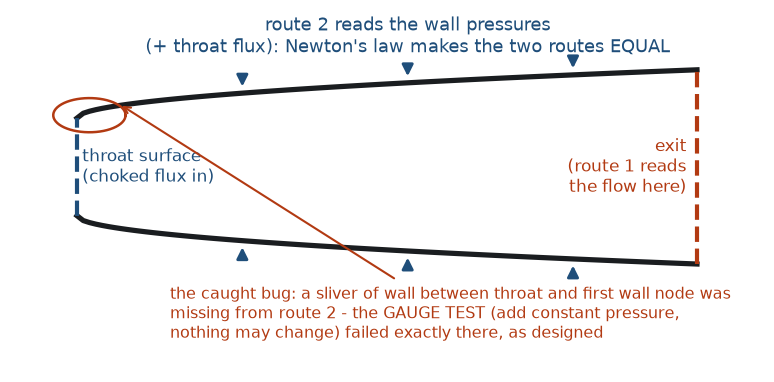
\includegraphics[width=0.82\textwidth]{sch_two_routes.png}
\caption{Due vie indipendenti verso un'unica spinta, disegnate nelle
coordinate proprie dell'ugello ($x$ [m] lungo l'asse, $y$ [m]
raggio). La via~1 (a destra) chiude la superficie di controllo sul
piano di uscita e richiede solo lo stato uniforme di uscita: portata
per velocità di uscita più $(p_e-p_a)A_e$. La via~2 (a sinistra e
lungo la parete) la chiude sulla macchina: flusso di quantità di
moto attraverso la gola bloccata più la spinta assiale di pressione
$(p-p_a)\,2\pi y\,\mathrm{d}y$ di ogni anello di parete. Si guardi a
ciò che le due vie \emph{non} condividono: nessuna quantità è usata
da entrambe, quindi la loro differenza $R_{\rm mom}$ [N] è un
autentico misuratore d'errore e non un'identità. Il cerchio rosso
segna la scheggia di superficie lasciata inizialmente aperta per
sbaglio, la cui storia è raccontata
nell'Appendice~\ref{app:sliver}.}
\label{fig:tworoutes}
\end{figure}

\subsection{Che cosa è stato costruito}

\carrier{validation/a1\_thrust\_functional.py}: entrambe le vie, il
residuo di quantità di moto $R_{\rm mom}$ con la sua banda di
Richardson, il test di gauge, $\mathrm{d}J/\mathrm{d}P$ in modo
inverso verificato manopola per manopola contro differenze finite
centrate, e tre rigettatori --- versioni deliberatamente corrotte
del calcolo (termine pressione--area eliminato, superficie non
chiusa, flusso corrotto) che la suite deve cogliere.

\subsection{Risultati di riferimento}

\textbf{8/8 PASS.} $J = 1.2552079\times10^{8}$~N; $R_{\rm mom} =
+2.85\times10^{3}$ contro una banda derivata di
$4.01\times10^{4}$ ($3.2\times10^{-4}$ di $J$), quindi le due vie
concordano a circa tre parti su diecimila della spinta; il rapporto
grossolana/fine dei residui pari a 4.52 è il $\approx 4$ atteso da
uno schema del secondo ordine quando la risoluzione viene
raddoppiata, il che conferma che ciò che resta è errore di
discretizzazione e non un errore concettuale. Scarto di gauge
$3.35\times10^{-8}$ contro $1.78\times10^{-6}$ ammesso: aggiungere
una pressione costante davvero non cambia nulla. Tutte e quattro le
componenti del gradiente cadono dentro le rispettive bande da
differenze finite ($\mathrm{d}J/\mathrm{d}y_t$ concorda a 9 cifre
significative), e tutti i rigettatori scattano.

Anche i segni del gradiente si comportano come la teoria prevede:
$\mathrm{d}J/\mathrm{d}\varepsilon > 0$ contro il vuoto, cioè
quando nulla spinge in senso contrario conviene sempre costruire un
ugello più lungo; e $\mathrm{d}J/\mathrm{d}r_{td}$ è minuscolo,
cioè la curvatura del breve raccordo appena a valle della gola conta
pochissimo. Un difetto reale è stato colto e corretto lungo la
strada: Appendice~\ref{app:sliver}.

\section{Il misuratore di ottimalità}
\label{sec:corner}

\subsection{La domanda}

Un punteggio e una bussola trovano progetti migliori. Che cosa
\emph{certifica} che un dato progetto soddisfa già la condizione che
un ottimo deve soddisfare?

\subsection{Come funziona, per esteso}

Scegliere la migliore parete di ugello non è un problema di trovare
il valore migliore di pochi numeri, ma di trovare la migliore
\emph{curva}; il ramo della matematica che se ne occupa è il
\emph{calcolo delle variazioni}, che si chiede che cosa debba essere
vero di una curva se nessuna sua piccola deformazione può migliorare
l'obiettivo. Rao~\cite{rao} risolse quel problema per un ugello e
trovò, fra le condizioni, un'affermazione scalare esatta che deve
valere al labbro --- il punto in cui la parete si ferma. È una
condizione \emph{terminale} (o di trasversalità):
\begin{equation}
R_{\rm corner}(p_a) \;=\; (p - p_a)\;-\;\tfrac{1}{2}\rho W^{2}
\sin(2\theta)\tan\alpha .
\label{eq:corner}
\end{equation}
La si legga come il bilancio dei due effetti dello spostare il
labbro di un passo più a valle. Il primo termine è il guadagno
diretto: un anello di parete in più, che conviene costruire finché
la pressione su di esso supera l'ambiente. Il secondo è il prezzo:
la parete aggiuntiva costringe il flusso a continuare a ruotare, e
il costo di quella rotazione è scritto attraverso l'angolo locale
del flusso $\theta$ (la direzione della velocità rispetto all'asse)
e l'angolo di Mach $\alpha$ (l'inclinazione delle linee lungo cui
viaggiano le perturbazioni supersoniche,
Capitolo~\ref{ch:moc}). $R_{\rm corner} = 0$ significa ``la parete
si ferma esattamente nel punto giusto'': un anello in più
guadagnerebbe quanto costa. Il misuratore valuta questa quantità dai
dati di labbro della marcia stessa, così che qualunque progetto il
motore produca possa essere certificato e non soltanto valutato.
Mediata sul ciclo del motore diventa la condizione di labbro che
l'ugello di un motore a detonazione rotante deve soddisfare
(affermazione T7 di~\cite{theory}), che il Capitolo~\ref{ch:cycle}
mette su un misuratore dedicato.

Lo strumento compagno è il \emph{primo integrale}
\begin{equation}
f_2 \;=\; \frac{W\cos(\theta-\alpha)}{\cos\alpha} \;=\; -\lambda_2 ,
\label{eq:f2}
\end{equation}
dove ``primo integrale'' significa una combinazione di grandezze di
flusso che le equazioni del moto obbligano a restare costante lungo
una particolare curva, benché ciascun ingrediente vari. La teoria di
Rao rende $f_2$ costante lungo la \emph{caratteristica terminale} di
un ugello ottimale --- l'ultima delle due famiglie di linee lungo
cui viaggia l'informazione supersonica, quella che chiude il campo
di moto al labbro. Il suo valore costante è $-\lambda_2$, un
\emph{moltiplicatore di Lagrange}: il numero che dà il prezzo di un
vincolo in un'ottimizzazione vincolata, qui indicando quanta spinta
si guadagnerebbe per ogni unità di portata in più concessa. Lungo
qualunque altra curva --- in particolare lungo la parete, che è una
\emph{linea di corrente}, cioè una linea ovunque tangente alla
velocità e dunque il percorso seguito da una particella di gas ---
$f_2$ \emph{non} è costante. Questo fornisce il controllo negativo
naturale: un'implementazione che facesse apparire $f_2$ costante
ovunque sarebbe rotta, e va colta.

\subsection{Che cosa è stato costruito}

\carrier{validation/a1\_corner\_instrument.py}: il misuratore di
spigolo e lo strumento $f_2$, verificati contro tre risposte note
sul caso dell'ugello ideale (uscita assiale, ambiente adattato,
vuoto), con il rigettatore di non costanza sulla parete.

\subsection{Risultati di riferimento}

\textbf{5/5 PASS} (82~s). L'angolo del flusso al labbro è zero di
macchina ($\theta = -10^{-16}$~rad: l'uscita è davvero assiale, come
l'ugello ideale assume). Con l'ambiente posto uguale alla pressione
di uscita il misuratore segna $3.7\times10^{-10}$ contro 42.8~Pa
ammessi --- l'ugello è certificato stazionario al suo ambiente di
progetto. Contro il vuoto segna esattamente $+p_e$, cioè
``allungami'', l'affermazione che nessun ugello finito è ottimale
nel vuoto, ora su un quadrante; e il suo segno concorda con un
$\mathrm{d}J/\mathrm{d}\varepsilon$ ricalcolato in modo
indipendente, così misuratore e gradiente raccontano la stessa
storia. Il primo integrale $f_2$ al labbro è uguale alla velocità di
uscita a meno di $4.6\times10^{-13}$~m/s, mentre lungo la parete
varia di 1173~m/s --- il rigettatore di non costanza, che scatta
come previsto.

\chapter{La prima ottimizzazione, contro una risposta nota}
\label{ch:firstopt}

Il capitolo precedente ha dato al motore un punteggio e una bussola.
Questo chiude l'anello per la prima volta: una ricerca che propone
progetti, li valuta con la marcia e prosegue finché non riesce più a
migliorare. Il punto non è la risposta ma la verifica --- il
problema è posto così piccolo che la sua soluzione è nota in anticipo
sulla carta, così la macchina può esservi confrontata. Un anello che
atterra su una risposta nota pur non sapendone nulla è degno di
fiducia su problemi la cui risposta non è nota.

\section{La domanda}

L'anello si chiude? Proporre, valutare, cercare --- e atterrare dove
la teoria dice che sta l'ottimo?

\section{Come funziona, per esteso}

La prima ottimizzazione è deliberatamente unidimensionale, così che
la sua risposta esista in forma chiusa (una formula esatta, in
contrapposizione a un numero ottenuto per iterazione). L'unica
manopola è il \emph{rapporto di espansione} $\varepsilon = A_e/A_t$
--- l'area di uscita divisa per l'area di gola, l'unico numero che
dice quanto l'ugello lascia espandere il gas
(Capitolo~\ref{ch:nozzle}). Tutto il resto è tenuto fisso.

La risposta nota viene dal lemma dell'area di uscita. Si derivi la
spinta~\eqref{eq:route1} rispetto all'area di uscita di un ugello
ideale (a uscita uniforme): allargare l'uscita di $\mathrm{d}A_e$
aggiunge un anello di parete su cui la pressione locale di uscita
$p_e$ spinge in avanti, mentre la pressione ambiente $p_a$ spinge
all'indietro sullo stesso anello, quindi
\begin{equation}
\frac{\mathrm{d}J}{\mathrm{d}A_e} \;=\; p_e - p_a
\qquad\Longrightarrow\qquad
\text{ottimo esattamente dove } p_e(\varepsilon^{*}) = p_a .
\label{eq:arealemma}
\end{equation}
Un ugello il cui gas è ancora sopra l'ambiente all'uscita
($p_e > p_a$) si dice \emph{sotto-espanso}: non ha finito di
espandersi e conviene allungarlo. Una volta che il gas è stato
espanso sotto l'ambiente ($p_e < p_a$) l'ugello è
\emph{sovra-espanso}: l'ambiente circostante spinge ora all'indietro
più forte di quanto il gas spinga in avanti su ogni nuovo anello, e
ogni anello aggiuntivo costa spinta. L'ottimo è il punto di
attraversamento. Porre una pressione ambiente fissa dunque
$\varepsilon^{*}$ analiticamente --- la marcia deve solo essere
invertita per trovare il rapporto di espansione a cui la sua
pressione di uscita eguaglia quell'ambiente.

La ricerca in sé non sa nulla di tutto questo. È una \emph{ricerca a
sezione aurea}: un metodo senza derivate che mantiene un intervallo
$[a,b]$ noto per contenere il massimo, valuta l'obiettivo in due
punti interni collocati secondo la sezione aurea, scarta l'estremo
che non può contenere il massimo e ripete finché l'intervallo non è
più stretto di una tolleranza fissata. Ogni restringimento riusa una
delle due valutazioni precedenti, ed è questo che la sezione aurea
fa guadagnare. I suoi unici ingressi sono chiamate alla marcia e
letture di $J$ --- nessun gradiente, nessuna conoscenza del lemma.
Ogni valutazione della marcia è memorizzata su disco con chiave
$\varepsilon$, così un'esecuzione interrotta riprende a costo nullo,
e il paesaggio della Figura~\ref{fig:jeps} è disegnato dalle
valutazioni della ricerca stessa anziché da una spazzata separata.

La suite chiude poi tre anelli indipendenti attorno alla risposta.
Il rapporto di espansione trovato dalla ricerca alla cieca deve
coincidere con la forma chiusa. La pressione di uscita lì deve
eguagliare l'ambiente posto, entro una banda derivata dalla stima
d'errore a due risoluzioni della marcia stessa più l'ampiezza
dell'intervallo su cui la ricerca si è fermata. E il misuratore di
spigolo della Sezione~\ref{sec:corner} --- costruito due passi
prima, mai consultato dalla ricerca --- deve leggere zero in modo
indipendente sul progetto trovato.

\section{Che cosa è stato costruito}

\carrier{validation/a1\_driver\_eps.py}: il driver a sezione aurea,
la cache su disco, le tre verifiche di chiusura e un rigettatore ---
un obiettivo deliberatamente corrotto, con il termine
pressione--area $(p_e-p_a)A_e$ cancellato, che deve allora correre
monotonamente fino al bordo dell'intervallo invece di trovare un
ottimo interno, perché senza quel termine nulla penalizza mai la
sovra-espansione.

\section{Risultati di riferimento}

\textbf{4/4 PASS} (231~s, 13 valutazioni della marcia). La ricerca
alla cieca atterra a $\varepsilon = 5.1551$ contro il valore
analitico $5.1506$; la pressione di uscita all'ottimo trovato
coincide con l'ambiente posto a meno di 916~Pa, dentro una banda
derivata di 7958~Pa; il misuratore di spigolo legge lì
indipendentemente $\approx 0$, quindi la condizione di ottimalità
della teoria di Rao è soddisfatta su un progetto raggiunto dalla
ricerca senza che essa l'abbia mai valutata; e l'obiettivo corrotto
corre fino al bordo dell'intervallo --- rigettato.

\begin{figure}[htbp]
\centering
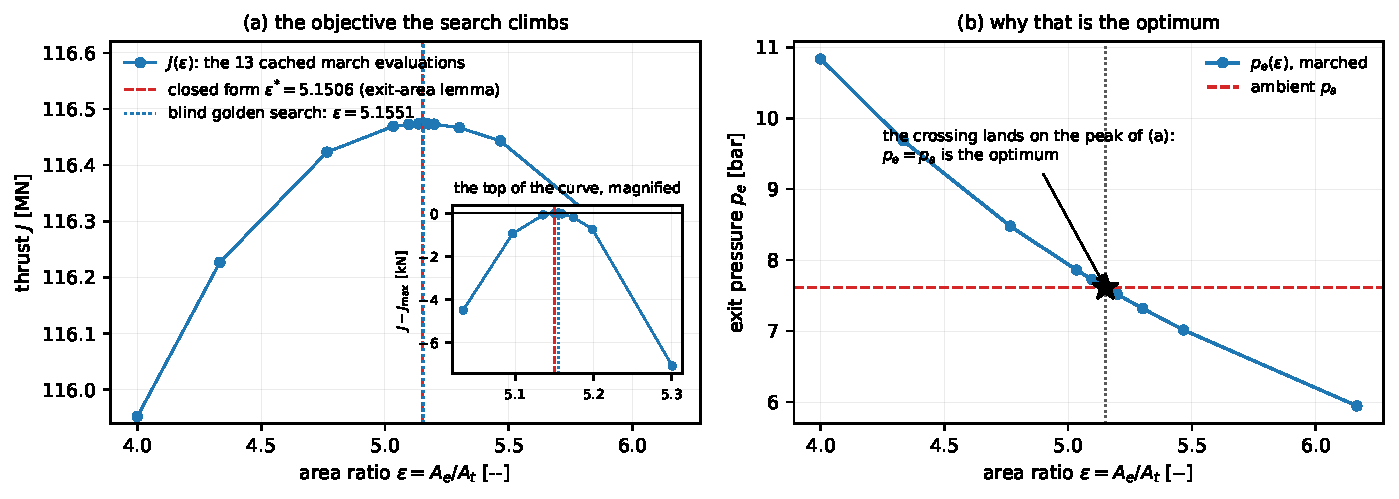
\includegraphics[width=0.8\textwidth]{fig_jeps.pdf}
\caption{Il paesaggio di ottimizzazione e la fisica dietro al suo
picco, entrambi disegnati dalle 13 valutazioni della marcia
memorizzate dal driver stesso. (a)~Spinta contro forma: rapporto di
espansione $\varepsilon$ [--] sull'asse orizzontale, obiettivo $J$
[MN] su quello verticale. Si osservi quanto è piatta la sommità ---
l'ottimo in forma chiusa (rosso tratteggiato) e il punto di
atterraggio della ricerca alla cieca (blu punteggiato) differiscono
dello 0.09\% in $\varepsilon$ su una curva piatta a parti su
$10^{5}$, quindi la ricerca alla cieca rinuncia a meno di $10^{-5}$
della spinta. (b)~Perché il picco stia lì: pressione di uscita $p_e$
[bar] contro lo stesso $\varepsilon$ [--], in calo attraverso la
linea della pressione ambiente $p_a$. L'attraversamento --- gas che
esce sopra l'ambiente a sinistra (sotto-espanso, allungare), sotto
l'ambiente a destra (sovra-espanso, accorciare) --- cade sullo
stesso $\varepsilon$ del picco in (a). È il lemma dell'area di
uscita, misurato anziché assunto.}
\label{fig:jeps}
\end{figure}

\chapter{La parete diventa un ingresso}
\label{ch:wallinput}

Finora il solutore ha disegnato da sé la propria parete di ugello:
la forma usciva dal calcolo, e l'unico modo di cambiarla era
cambiare le poche manopole che guidano la costruzione. Un
ottimizzatore che debba esplorare forme libere ha bisogno del flusso
di dati rovesciato --- gli si consegna una parete qualunque e se ne
ottiene il flusso su quella parete. Questo capitolo esegue quella
inversione usando gli stessi mattoni già verificati, confronta il
nuovo motore con quello vecchio sull'unica parete che entrambi
sanno trattare, e certifica la derivata della spinta rispetto a una
deformazione arbitraria della parete. È quella derivata la bussola
di ogni ottimizzazione successiva di questo documento.

\section{La domanda}

La marcia del Mattone~1 \emph{disegna} la propria parete: il
contorno è calcolato come una \emph{linea di corrente} --- una linea
ovunque tangente alla velocità locale, il percorso seguito da una
particella di gas --- scelta in modo che al suo interno passi
esattamente la portata di gola. In altre parole la parete è
un'uscita. Il progetto a forma libera richiede l'opposto: si
consegna una parete \emph{qualsiasi} e se ne ottiene il flusso. Le
stesse celle già verificate sanno calcolare il flusso su una parete
assegnata?

\begin{figure}[htbp]
\centering
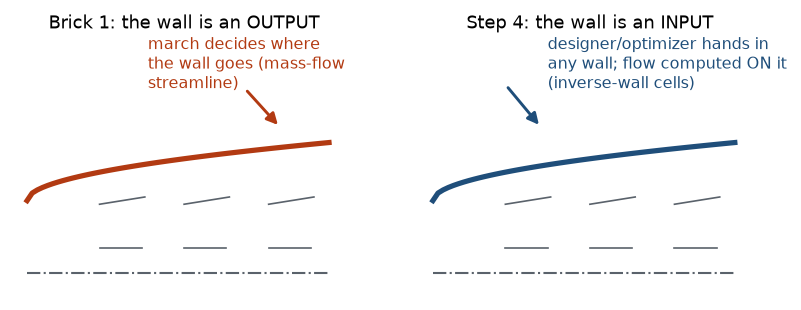
\includegraphics[width=0.86\textwidth]{sch_inversion.png}
\caption{L'inversione strutturale, disegnata in coordinate di ugello
($x$ [m] lungo l'asse, $y$ [m] raggio). A sinistra: il generatore
decide da sé la propria parete seguendo una linea di corrente di
portata, quindi la forma è un risultato. A destra: l'ottimizzatore
consegna una parete arbitraria e le celle di parete inversa ne
calcolano il flusso, quindi la forma è un dato. Si guardino le
frecce: ciò che cambia è soltanto la direzione in cui vengono
determinate la posizione di parete e lo stato del flusso --- tutto
ciò che sta a monte, e ogni cella interna al flusso, resta
invariato. È per questo che il nuovo motore eredita la
certificazione del vecchio.}
\label{fig:inversion}
\end{figure}

\section{Come funziona, per esteso}

Il motore lascia invariato tutto ciò che sta a monte della parete
--- stesso avvio in gola, stesso ventaglio di espansione iniziale ---
e cambia soltanto il modo in cui ciascuna colonna di punti calcolati
termina. Nel generatore il punto di parete è \emph{prodotto}: la
marcia integra la linea di corrente di portata e la parete è
ovunque essa vada. In modalità inversa la \emph{posizione} del punto
di parete è \emph{data} (deve trovarsi sul contorno assegnato in
quella stazione, con la pendenza locale del contorno fornita come
dato), quindi la cella di parete lavora all'indietro, esattamente
come descritto nel Capitolo~\ref{ch:moc}: trova il \emph{piede}
della \emph{caratteristica} in arrivo --- il punto sulla colonna
precedente da cui è partita la linea che porta informazione al punto
di parete --- con una ricerca per corde, scandendo i segmenti
memorizzati di quella colonna alla ricerca di quello i cui dati
racchiudono la condizione caratteristica. Chiude poi la relazione di
compatibilità lungo la corda dal piede al punto di parete, con la
pendenza assegnata della parete che vi fornisce la direzione del
flusso~\cite{zucrow}. Si costruisce una colonna di marcia per ogni
stazione di parete assegnata.

Due conseguenze danno forma al resto del motore. Primo, una parete
arbitraria non produce un'uscita uniforme e assiale, quindi nulla a
valle può assumerlo: la spinta è sempre valutata per la via di
parete~\eqref{eq:route2}, che richiede solo le pressioni di parete e
il flusso in gola. Secondo, l'intera costruzione resta
differenziabile --- la ricerca del piede, la chiusura sulla corda,
la quadratura della spinta --- quindi la differenziazione automatica
in modo inverso fornisce $\mathrm{d}J/\mathrm{d}({\rm parete})$, la
sensibilità della spinta a una variazione di parete a forma libera,
al costo di circa una marcia aggiuntiva.

Quel gradiente è certificato dall'\emph{identità dell'inviluppo},
che è il teorema fondamentale del calcolo usato come test: la media
di una derivata su un intervallo deve eguagliare la pendenza della
secante su quell'intervallo,
$\overline{\mathrm{d}J/\mathrm{d}a} = [J(a_2)-J(a_1)]/(a_2-a_1)$. Il
test deforma dunque la parete con una protuberanza liscia e
localizzata di ampiezza $a$, spazza $a$ su un intervallo, adatta una
retta ai campioni del gradiente AD e richiede che la pendenza media
adattata coincida con una secante ampia di $J$ stesso entro una
banda derivata. Perché non l'ovvio confronto puntuale fra AD e una
differenza finita a passo piccolo? Perché le proprietà del gas sono
lette da tabelle interpolate linearmente a tratti, quindi la
derivata esatta del codice porta un microscopico dente di sega alla
scala delle celle di tabella, e una differenza a passo piccolo si
mette a cavallo di quelle cuspidi: quel test è qui mal posto. Il
risultato e la sua diagnosi sono nell'Appendice~\ref{app:ripple}; il
certificato d'inviluppo ne è la soluzione e la
Figura~\ref{fig:ripple} il riassunto in un'immagine.

\begin{figure}[htbp]
\centering
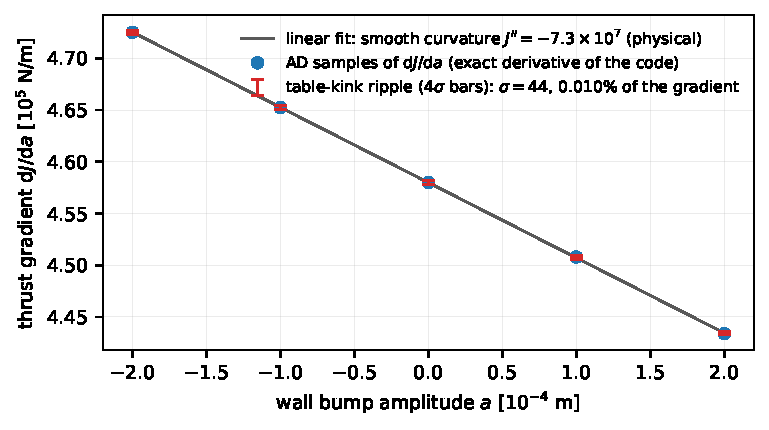
\includegraphics[width=0.72\textwidth]{fig_grad_ripple.pdf}
\caption{Perché il gradiente è certificato per inviluppo anziché
puntualmente. Asse orizzontale: ampiezza $a$ [m] della protuberanza
liscia aggiunta alla parete, da rientrante a sporgente. Asse
verticale: la sensibilità della spinta $\mathrm{d}J/\mathrm{d}a$
[N/m] restituita dalla differenziazione automatica, cioè newton di
spinta guadagnati per metro di protuberanza. Si guardino le due cose
sovrapposte: un andamento rettilineo e liscio (la retta; curvatura
adattata $J'' = -7.3\times10^{7}$~N/m$^2$), che è la fisica, e una
minuscola dispersione attorno a esso (barre rosse a $4\sigma$;
$\sigma = 44$~N/m, lo 0.010\% del gradiente), che è il motivo di
cuspidi delle tabelle di proprietà lineari a tratti. Entrambi sono
proprietà reali dell'obiettivo discreto --- l'AD riporta la derivata
esatta del codice, dente di sega compreso --- ma solo l'andamento è
fisico, ed è per questo che il certificato media sull'increspatura
invece di campionarla. Storia completa
nell'Appendice~\ref{app:ripple}.}
\label{fig:ripple}
\end{figure}

\section{Che cosa è stato costruito}

\carrier{validation/a1\_wall\_march.py}: il motore a parete
assegnata (\code{wall\_march}), l'estrattore di stazioni
(\code{stations\_from\_wall}), la spinta per via di parete
(\code{J\_wall}), il flusso di massa per colonna, il certificato di
gradiente per identità dell'inviluppo e i rigettatori (una parete i
cui dati di pendenza siano corrotti deve far fallire la marcia).

\section{Risultati di riferimento}

\textbf{Stadio gemello, 5/5 PASS.} Alimentato con il contorno del
Mattone~1 come parete assegnata, il nuovo motore riproduce la spinta
del Mattone~1 attraverso un calcolo completamente diverso ---
$J_{\rm wall} = 1.25534\times10^{8}$~N contro
$J_{\rm exit} = 1.25521\times10^{8}$~N, una differenza di
$1.37\times10^{4}$ dentro una banda derivata di $1.58\times10^{5}$.
La portata attraverso l'ultima colonna calcolata eguaglia la portata
di gola a meno di 12.3~kg/s (banda 152), una verifica di
conservazione indipendente che il confronto fra gemelli non
contiene; il numero di Mach minimo lungo la parete è 1.20, quindi il
flusso resta supersonico ovunque e il metodo resta applicabile;
17{,}221 celle sono certificate da Newton, cioè ogni risoluzione
locale è convergita dentro la propria banda derivata di residuo; e
la parete con pendenza corrotta fa fallire la marcia --- rigettata.
\textbf{Stadio gradiente, 2/2 PASS} per identità dell'inviluppo:
$|{\rm AD} - {\rm secante}| = 29$ contro una banda derivata di 109,
e la sensibilità è essa stessa molto maggiore di quella banda,
quindi la parete conta in modo dimostrabile.

\chapter{L'arbitro, e i moltiplicatori di Rao contro l'aggiunto}
\label{ch:referee}

Finora il programma ha verificato soltanto sé stesso. Questo capitolo
chiama in causa due giudici esterni: un codice di progetto di ugelli
scritto da altre persone in un altro linguaggio, i cui campi di moto
interi vengono sottoposti alle nostre equazioni, e la teoria del 1958
dell'ugello ottimale fatta con carta e matita, le cui previsioni
misuriamo su una forma che il nostro ottimizzatore non ha prodotto.
Superare entrambi significa che il motore risolve il problema giusto,
e non semplicemente un problema coerente con sé stesso.

\section{L'arbitro torna in linea}

\subsection{Che cosa occorre sapere prima}

Un ugello \emph{ideale}, o \emph{a lunghezza minima}, dà un flusso di
uscita perfettamente uniforme e puramente assiale nella minima
lunghezza in grado di farlo (Capitolo~\ref{ch:nozzle}). Un
\emph{contorno ottimizzato in spinta} (il TOC di Rao~\cite{rao})
risponde a una domanda diversa: per una \emph{data} lunghezza, quale
forma produce la massima spinta? È più corto e più pieno, il suo
flusso di uscita è deliberatamente non uniforme, e compra più spinta
per chilogrammo di ugello. Qui entrambe le forme raggiungono lo
stesso \emph{rapporto di espansione} $\varepsilon = A_e/A_t = 4$:
area di uscita quattro volte l'area di gola, il numero che dice
quanto l'ugello espande il gas. Ovunque, le tolleranze sono
\emph{bande derivate} calcolate dalla discretizzazione anziché
scelte, e ogni test porta con sé i \emph{rigettatori}: ingressi
corrotti che deve far fallire (Capitolo~\ref{ch:method}; simboli
nella Tabella~\ref{tab:notation}).

\subsection{La domanda}

Tutto quanto precede verifica il nostro codice contro sé stesso e
contro forme chiuse. Dov'è il programma \emph{indipendente} capace di
arbitrare interi campi di moto?

\subsection{Come funziona, per esteso}

GENO~\cite{geno} è quel programma: un progettista di ugelli in
Fortran indipendente --- base di codice separata, discretizzazione
separata, backend termodinamico separato --- e, per decisione
permanente, mai modificato da noi e mai differenziato. Come
\emph{generatore} produce contorni e campi di riferimento, in
particolare l'ugello ottimizzato in spinta di cui la
Sezione~\ref{sec:o33} ha bisogno: una forma genuinamente ottimale
nella cui produzione il nostro ottimizzatore non ha avuto parte. Come
\emph{arbitro}, i suoi campi vengono messi sotto processo contro le
\emph{nostre} equazioni. Il nostro solutore costruisce un flusso su
una maglia di linee d'onda intersecanti, imponendo in ogni punto di
maglia un insieme fissato di relazioni algebriche --- il suo
\emph{processo elementare} (Capitolo~\ref{ch:moc}); quelle relazioni
vengono ora valutate sui valori nodali di GENO, dove devono valere
entro la banda derivata. Il controllo è un insieme di \emph{piedi}
deliberatamente sbagliati --- i punti a monte, sulle due linee
d'onda, da cui un punto di maglia è costruito --- che \emph{non}
devono valere. L'accordo significa allora che i due codici risolvono
le stesse equazioni cella per cella, e non soltanto che le loro
uscite si somigliano.

Il vecchio binario di GENO era anteriore alla toolchain di questo
host, quindi è stato ricompilato dai sorgenti; il caso di riferimento
rigenerato è il TOC di tipo~2 a $\varepsilon = 4$ ($874\times2885$
nodi).

\subsection{Risultati di riferimento}

\begin{itemize}[itemsep=2pt]
\item \textbf{Oracolo fra codici: PASS.} 218/218 celle campionate del
  campo rigenerato soddisfano le nostre relazioni di processo
  elementare dentro la banda derivata, con una discriminazione
  $84\times$ fra piedi caratteristici corretti e deliberatamente
  sbagliati.
\item \textbf{Chiuso l'ultimo SKIP del Mattone~1.} Un test del
  Mattone~1 era ineseguibile finché l'arbitro non veniva compilato
  qui. Ora gira dal vivo, confrontando il nostro contorno ideale con
  quello di GENO stazione per stazione: 62/62 campioni in banda,
  errore massimo $7.6\times10^{-9}$~m.
\item \textbf{Il controllo positivo su $f_2$ è atterrato} (l'unico
  test dichiarato in sospeso della Sezione~\ref{sec:corner}). $f_2$
  combina velocità e direzione locali del flusso, e la teoria lo
  obbliga a essere costante lungo una linea di un ugello ottimale ---
  la \emph{caratteristica terminale}, definita più avanti. Sul
  contorno genuinamente ottimale di Rao è lì costante con una
  dispersione relativa di $4.0\times10^{-3}$ mentre lungo la parete
  varia di 0.60 --- una separazione $149\times$. Il caso di
  riferimento \emph{troncato} ha correttamente mostrato assenza di
  costanza: tagliato corto, un contorno ottimale non contiene più la
  propria superficie di controllo.
\end{itemize}

\begin{figure}[htbp]
\centering
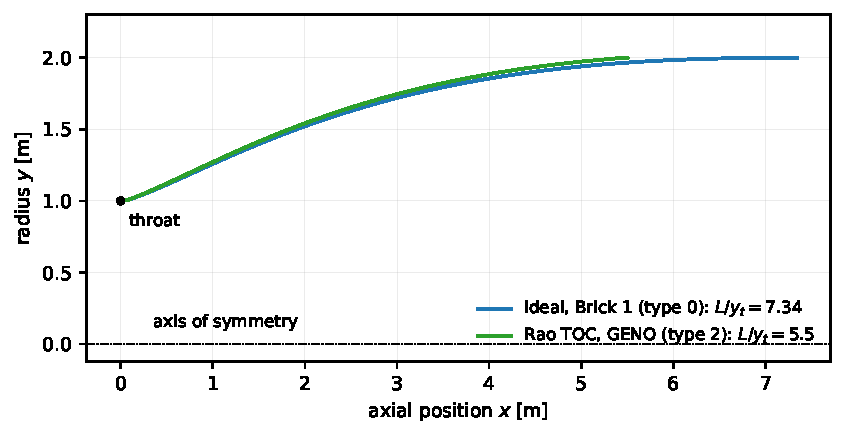
\includegraphics[width=0.85\textwidth]{fig_contours.pdf}
\caption{I due protagonisti, disegnati in scala: distanza assiale $x$
[m] contro raggio $y$ [m], asse di simmetria a $y = 0$, gola a
$x = 0$, $y = y_t = 1$~m (quindi qui metri e raggi di gola
coincidono). Entrambe le pareti raggiungono il rapporto di espansione
$\varepsilon = 4$; si guardino le \emph{lunghezze}. L'ugello ideale
(a lunghezza minima) del Mattone~1 arriva a $L = 7.3409$~m, il
contorno ottimizzato in spinta di Rao prodotto da GENO si ferma a
5.5~m: più corto per costruzione (massima spinta per una \emph{data}
lunghezza). Una verifica incrociata non pianificata: GENO ha
rifiutato una richiesta di TOC più lungo citando la lunghezza ideale
$L = 7.3409$ --- esattamente quella del nostro gemello, da un codice
che il nostro non l'ha mai visto.}
\label{fig:contours}
\end{figure}

\section{I moltiplicatori di Rao contro il nostro aggiunto, su un
contorno realmente ottimale}
\label{sec:o33}

\subsection{La domanda}

Rao risolse il problema dell'ugello ottimale nel 1958 con la carta e
il calcolo delle variazioni. Questo programma lo risolve per
\emph{differenziazione automatica}: la macchina propaga le derivate
attraverso ogni operazione che il solutore esegue, dando la
sensibilità esatta della spinta a ogni parametro di forma --- e
eseguita all'indietro (un \emph{aggiunto}) una sola passata le
restituisce \emph{tutte} in una volta, a circa il costo di una
risoluzione di flusso aggiuntiva. La voce aperta più antica del
registro (la sua C-O33 in~\cite{theory}) chiede se le due risposte
concordino, termine per termine, su un contorno realmente ottimizzato
in spinta.

\subsection{Come funziona, per esteso}

Il terreno d'incontro è il contorno ottimale di GENO, marciato dal
\emph{nostro} motore a parete assegnata
(Capitolo~\ref{ch:wallinput}). Quando qualcosa viene massimizzato
sotto vincoli, ogni vincolo entra nella soluzione con una costante
che ne dà il prezzo --- un \emph{moltiplicatore di Lagrange}. La
soluzione di Rao~\cite{rao} ne porta due: $\lambda_2$, il prezzo di
tenere fissa la portata, e $\lambda_3$, il prezzo di tenere fissa la
lunghezza. Ciascuno è falsificabile, perché la teoria nomina una
combinazione di grandezze locali del flusso che deve eguagliarlo in
ogni punto di una curva --- un \emph{primo integrale}, una quantità
che le equazioni tengono lì costante. Quella curva è la
\emph{caratteristica terminale}: l'ultima linea d'onda $C^{-}$
dell'ugello, dall'asse al labbro, la superficie di controllo che il
calcolo delle variazioni seleziona perché spinta e portata vengono
valutate attraverso di essa. Lì:
\begin{equation}
f_2 = \frac{W\cos(\theta-\alpha)}{\cos\alpha} = -\lambda_2 ,
\qquad
2\pi y\,\rho W^{2}\sin^{2}\theta\,\tan\alpha = -\lambda_3 ,
\label{eq:firstintegrals}
\end{equation}
con $W$ il modulo della velocità [m/s] (il $q$ della
Tabella~\ref{tab:notation}), $\theta$ l'angolo del flusso, $\alpha$
l'angolo di Mach, $\rho$ la densità, $y$ il raggio --- entrambi
\emph{costanti lungo quella curva} se e solo se il contorno è
ottimale. Il test campiona entrambe le quantità sui nodi della
caratteristica terminale di GENO e richiede costanza entro bande
derivate nel nostro campo \emph{e} in quello di GENO, più l'accordo
fra i codici sugli stessi nodi.

Il lato aggiunto verifica la \emph{stazionarietà}, l'enunciato del
calcolo per lo stare su un massimo: in un massimo la derivata in ogni
direzione \emph{ammessa} si annulla, quindi piccole variazioni
ammesse non costano nulla al primo ordine. Le direzioni ammesse sono
deformazioni di parete che tengono fissi la lunghezza ed entrambi gli
estremi --- sei protuberanze gaussiane con estremi bloccati (centri
da $0.20L$ a $0.85L$). Una protuberanza che sposti il labbro sonda
una direzione che la teoria non protegge (un ugello più grande paga
sempre un poco di più) e deve dare un gradiente grande; le stesse sei
protuberanze su una parete deliberatamente perturbata sono il
controllo positivo. Ogni proiezione AD è verificata contro differenze
finite, cioè contro il ricalcolo della spinta con la forma spostata a
mano.

\subsection{Risultati di riferimento}

\textbf{9/9 PASS su due stadi}
(\carrier{validation/a1\_o33\_toc.py}). \emph{Integrali}: il nostro
campo sui nodi della caratteristica terminale di GENO mostra $f_2$
costante con dispersione relativa $4.045\times10^{-3}$ (quella di
GENO: $4.04\times10^{-3}$), e il livello coincide fra i codici a meno
di 0.235~m/s su 2634.7~m/s --- $9\times10^{-5}$ relativo
(Figura~\ref{fig:f2}); $\lambda_3$ coincide punto per punto (la sua
costanza è onestamente dichiarata irrisolvibile a questa precisione
di superficie: $\lambda_3 \sim \sin^{2}\theta$ è piccolo e ripido
vicino all'asse). \emph{Stazionarietà}: i sei gradienti interni
stanno $1000\times$ sotto la direzione del labbro e $40\times$ sotto
i gradienti sulla parete perturbata, AD${}={}$FD entro l'${\sim}1\%$
ovunque, e il contorno ottimale batte quello perturbato,
$J({\rm TOC}) > J({\rm perturbato})$
(Figura~\ref{fig:stationarity}). Un rigettatore è stato esso stesso
corretto dalla fisica lungo la strada:
Appendice~\ref{app:f2rejector}. Lo scarico formale del registro
(YAML e cablaggio della suite) è un atto da eseguire al momento del
commit sul repository WSL; il contenuto numerico esiste.


\begin{figure}[htbp]
\centering
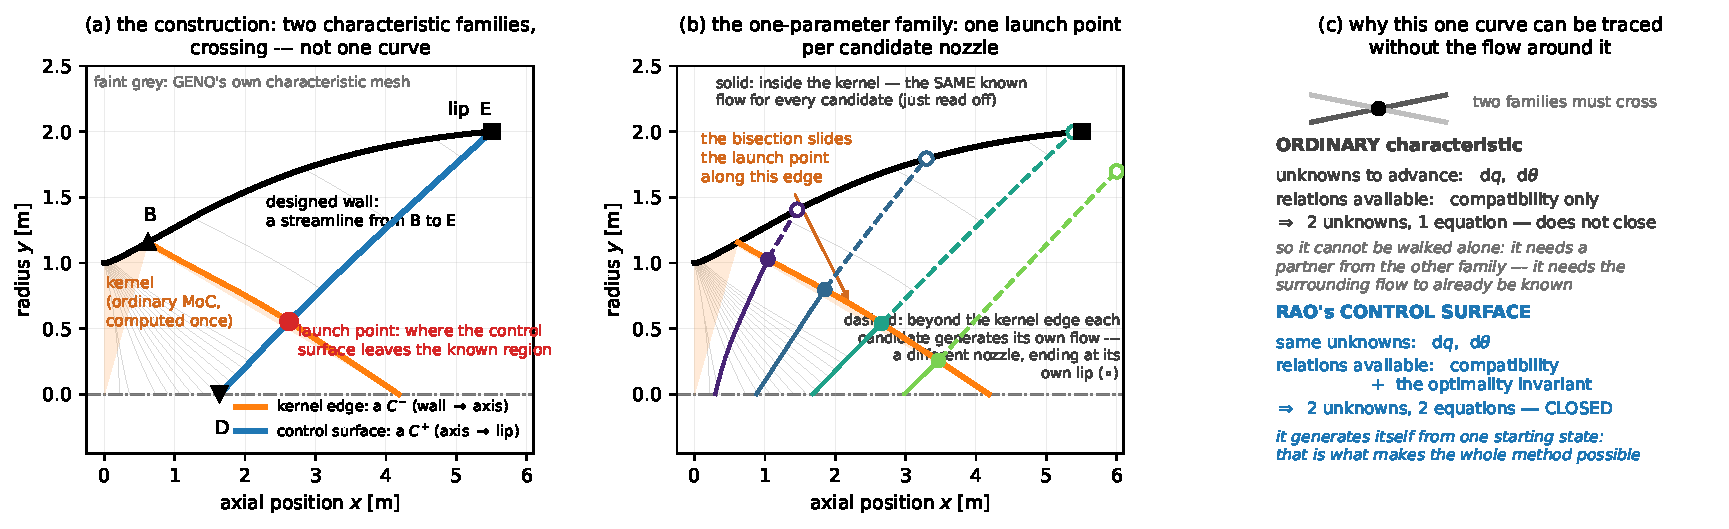
\includegraphics[width=\textwidth]{fig_rao_construction.pdf}
\caption{Come viene realmente costruita la superficie di controllo
ottimale di Rao, disegnata sul campo realmente ottimizzato in spinta
(assi: posizione assiale e raggio in metri; le tenui linee grigie
sono la maglia caratteristica del codice di riferimento). (a)~Due
famiglie caratteristiche che si \emph{incrociano}: il bordo del
nucleo (arancione), una $C^{-}$ che corre dalla fine dell'espansione
iniziale in B giù fino all'asse, e la superficie di controllo (blu),
una $C^{+}$ che corre da D sull'asse su fino al labbro E. Il punto
rosso è il punto di lancio, dove la superficie di controllo lascia la
regione che la gola già determina. Tutto ciò che sta dentro il nucleo
ombreggiato è marcia ordinaria, calcolata una volta sola. (b)~La
famiglia a un parametro: ogni punto di lancio sul bordo del nucleo dà
un ugello candidato diverso. Linea continua dentro il nucleo --- lo
stesso flusso noto per ogni candidato; tratteggiata oltre, dove
ciascuno genera il proprio flusso e finisce al proprio labbro. La
ricerca fa scorrere il punto di lancio lungo quel bordo. (c)~Perché
questa singola curva possa essere tracciata senza conoscere il flusso
attorno a essa: una caratteristica ordinaria ha due incognite da
avanzare e solo la relazione di compatibilità per avanzarle, quindi
ha bisogno di una compagna dell'altra famiglia; la condizione di
ottimalità di Rao fornisce la seconda relazione mancante, e il
sistema si chiude.}
\label{fig:raoconstruction}
\end{figure}

\begin{figure}[htbp]
\centering
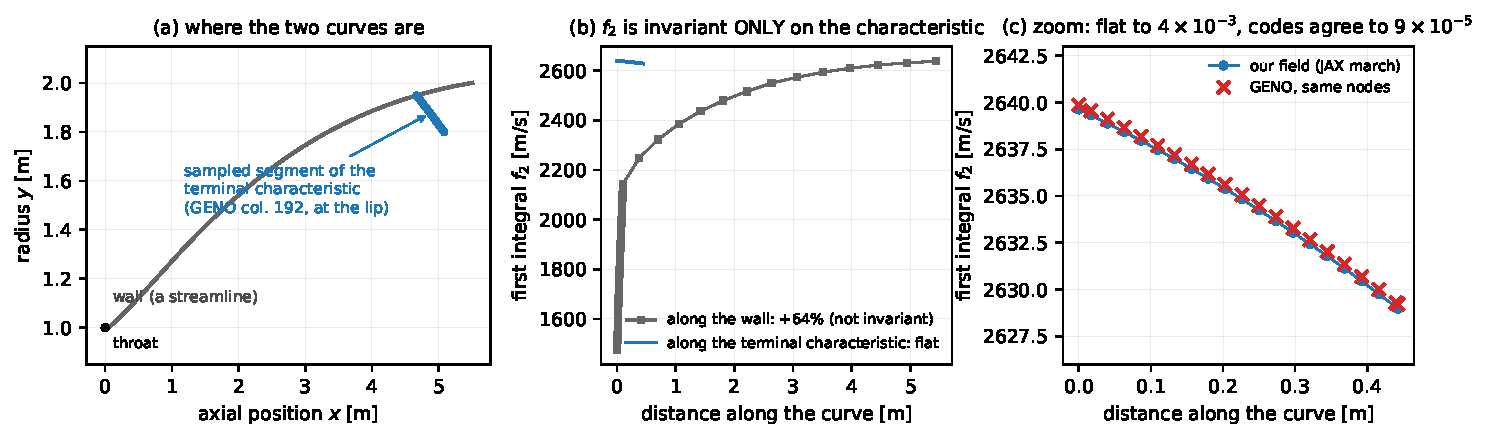
\includegraphics[width=\textwidth]{fig_f2.pdf}
\caption{Il primo integrale, misurato. (a)~Dove vivono le due curve:
$x$ [m] contro $y$ [m] sull'ugello ottimizzato in spinta di GENO ---
la parete (grigio) e il tratto campionato della caratteristica
terminale, la sua ultima linea d'onda (blu). (b)~$f_2$ [m/s] contro
ascissa curvilinea [m] lungo ciascuna curva: sale del 64\% lungo la
parete --- lì nessun invariante, e la teoria dice che non deve
esserci --- e resta piatto lungo la caratteristica terminale.
(c)~Ingrandimento su quella linea piatta, stesse unità: il nostro
campo (cerchi) si sovrappone a quello di GENO (croci) sugli stessi
nodi. Piattezza a $4\times10^{-3}$ relativi con accordo fra codici a
$9\times10^{-5}$: la costante $-\lambda_2$ di Rao esiste in un flusso
calcolato, e due codici senza rapporto fra loro ne trovano lo stesso
valore.}
\label{fig:f2}
\end{figure}

\begin{figure}[htbp]
\centering
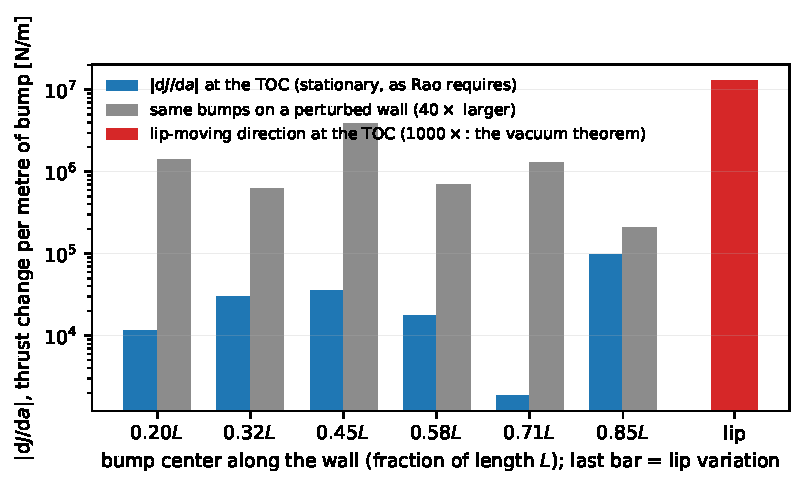
\includegraphics[width=0.8\textwidth]{fig_stationarity.pdf}
\caption{Stazionarietà, in scala logaritmica. Asse orizzontale: la
deformazione di parete applicata --- sei protuberanze gaussiane,
etichettate dal loro centro come frazione $x/L$ [--] della lunghezza
di parete, più la deformazione che sposta il labbro. Asse verticale:
$|\mathrm{d}J/\mathrm{d}a|$ [N/m], variazione di spinta per metro di
ampiezza della protuberanza, logaritmico. Sul contorno ottimale (blu)
il gradiente sta $40\times$ sotto le stesse protuberanze su una
parete deliberatamente perturbata (grigio) e $1000\times$ sotto la
direzione del labbro (rosso): piatto nelle direzioni ammesse, ripido
nell'unica direzione che la teoria non protegge. È così che un ottimo
appare all'aggiunto.}
\label{fig:stationarity}
\end{figure}

\chapter{Lo strato di ciclo: il motore diventa uno strumento per RDE}
\label{ch:cycle}

Finora l'ugello aveva un solo punto di funzionamento: una pressione
di camera, una temperatura di camera, un progetto. Un motore a
detonazione rotante non ne offre uno solo. Questo capitolo insegna
all'ottimizzatore a progettare rispetto a un intero ciclo periodico
di condizioni di camera --- e dimostra poi che lo ha fatto
correttamente, facendogli riprodurre alla cieca due risposte che la
teoria già conosce e che un'implementazione con scorciatoie non
potrebbe trovare.

\section{Ottimizzazione mediata sul ciclo e i suoi oracoli}

\subsection{Che cosa occorre sapere prima}

Un \emph{motore a detonazione rotante} (RDE) brucia il proprio
propellente in una camera anulare attorno alla quale una o più
\emph{onde di detonazione} --- fronti di combustione supersonici, un
urto con la fiamma agganciata a esso --- corrono di continuo, tipicamente
qualche migliaio di volte al secondo, con propellente fresco che
riempie lo spazio dietro ciascuna onda. La conseguenza per l'ugello è
il punto di questo capitolo: una sezione di ugello non vede mai
condizioni stazionarie. Una volta per giro la pressione salta
bruscamente al passaggio dell'onda, poi cala (\emph{si svuota}) fino
all'arrivo dell'onda successiva.

Ciò a cui l'ugello risponde è lo \emph{stato di ristagno}
$(P_0, T_0)$: la pressione e la temperatura che il gas di camera
avrebbe se portato dolcemente a riposo, la condizione di serbatoio
che fissa tutto ciò che sta a valle. In un RDE è una \emph{famiglia}
periodica $(P_0(\xi), T_0(\xi))$ indicizzata dalla \emph{fase di
ciclo} $\xi \in [0,1]$, un giro completo dell'onda; la \emph{misura
di fase} $\mathrm{d}\mu(\xi)$ dice quanta parte del ciclo occupa
ciascuna fase, e dunque il suo peso in una media. E
\emph{quasi-stazionario} significa che il gas attraversa l'ugello in
un tempo molto minore di quello che l'onda impiega a ritornare ---
cosicché in ogni istante il flusso è semplicemente il flusso
stazionario dello stato di camera di quell'istante. La variabile di
progetto è ovunque il rapporto di espansione
$\varepsilon = A_e/A_t$, area di uscita su area di gola
(Capitolo~\ref{ch:nozzle}).

\subsection{La domanda}

Un RDE consegna all'ugello una \emph{famiglia} periodica di stati di
camera, non uno solo. Il motore sa ottimizzare la spinta mediata sul
ciclo --- e dimostrare di farlo correttamente?

\subsection{Come funziona, per esteso}

Poiché l'espansione è quasi-stazionaria, la spinta mediata sul ciclo
è semplicemente la media in fase delle spinte stazionarie:
\begin{equation}
J_{\rm cycle}(\varepsilon) \;=\; \int_0^1
F\!\left(\varepsilon;\, P_0(\xi),\, T_0(\xi)\right)\mathrm{d}\mu(\xi).
\label{eq:jcycle}
\end{equation}
Lo strato implementa questa formula \emph{onestamente}: l'integrale è
una quadratura su un insieme finito di fasi, e ogni fase riceve il
proprio stato di ristagno costruito sulle stesse tabelle di gas, la
propria marcia completa attraverso l'ugello e la propria spinta. Da
nessuna parte è programmata una scorciatoia che sfrutti una
similitudine fra le fasi --- deliberatamente, perché il test più
difficile della teoria riguarda proprio ciò che
un'implementazione onesta deve allora riprodurre da sé.

Quel test è il teorema di collasso per la campana fissa (la sua
T3)~\cite{theory}. Dice: se sul ciclo varia solo la pressione e non
la temperatura (uno svuotamento \emph{a sola pressione}, $T_0$
fisso), l'intero problema di ciclo collassa su un classico progetto
stazionario alla pressione media --- quindi l'ottimizzazione
consapevole del ciclo deve comprare \emph{esattamente nulla}. La
ragione è una similitudine: a $T_0$ fisso e geometria fissa, scalare
$P_0$ scala ogni pressione nell'ugello dello stesso fattore e non
muove né pareti né numeri di Mach, quindi $J_{\rm cycle}$ è
esattamente il $J$ stazionario a $\langle P_0\rangle$. Un motore che
marcia ogni fase in modo indipendente non ha modo di saperlo --- a
meno che non sia corretto, nel qual caso il guadagno nullo
\emph{emerge}. Quell'emergere è il test.

Il secondo stadio pone il primo RDE simulato (posto dall'utente):
profili esponenziali in fase di $P_0$ \emph{e} $T_0$ (rapporto di
pressione picco-valle $PR = 10$, rapporto di temperatura
$TR = 1.306$, picco 3850~K, cinque fasi equispaziate nel logaritmo
della pressione). Con $T_0$ variabile il collasso non è più esatto, e
la domanda diventa quantitativa: quanto si avvicina all'ottimo di
ciclo trovato alla cieca il miglior progetto \emph{a un solo numero}
--- un ordinario progetto a punto singolo su uno stato di camera
rappresentativo --- e qual è lo stato giusto? La risposta della
teoria --- la pressione media alla temperatura \emph{pesata sulla
pressione} $\langle P T\rangle/\langle P\rangle$ --- viene
confrontata con l'alternativa della media logaritmica in un paragone
derivato, e un progetto fatto alla fase di picco di pressione
fornisce il riferimento deliberatamente sbagliato.

Costruire lo stato di ristagno di una fase su proprietà di gas reale
tabulate ha trappole proprie; le tre incontrate (e i rigettatori che
ora le presidiano) sono nell'Appendice~\ref{app:cycletraps}.

\subsection{Risultati di riferimento}

\textbf{L'oracolo del collasso a guadagno nullo: 5/5 PASS}
(\carrier{validation/a1\_cycle\_layer.py}, stadio \code{t3}).
L'ottimizzatore, cui non è stato detto nulla del teorema e che spende
cinque marce complete per ogni valutazione dell'obiettivo, atterra
sul progetto-alla-media entro la propria finestra: il guadagno che
trova rispetto a quel progetto è di $-475$~N su
$1.16\times10^{8}$~N, contro una banda derivata di
$9.6\times10^{3}$~N --- zero, alla precisione che il test può
risolvere. Il progetto deliberatamente sbagliato alla pressione di
picco perde $4.8\times10^{6}$~N, $500\times$ la banda, quindi un
guadagno reale si sarebbe visto. E la similitudine si manifesta dal
vivo: a geometria fissa le cinque pareti per fase coincidono a meno
di $8.9\times10^{-16}$ --- scalare la pressione non muove la parete,
misurato allo zero di macchina.

\textbf{L'RDE simulato: 6/6 PASS} (stadio \code{mock}). L'ottimo
trovato alla cieca cade entro il $-0.74\%$ in $\varepsilon$ rispetto
al miglior progetto a un solo numero --- che è appunto la pressione
media alla temperatura pesata sulla pressione
$\langle PT\rangle/\langle P\rangle$, battendo il riferimento a media
logaritmica in un paragone derivato (la lezione della media pesata
della teoria, confermata a livello di motore); la penalità di spinta
di quel progetto a un solo numero è $2.5\times10^{-6}$ relativa
(secondo ordine, come previsto), mentre il progetto di picco perde il
4\% di $J$. La lettura pratica: per questa classe di cicli uno stato
ben scelto basta, e la teoria dice quale.

\begin{figure}[htbp]
\centering
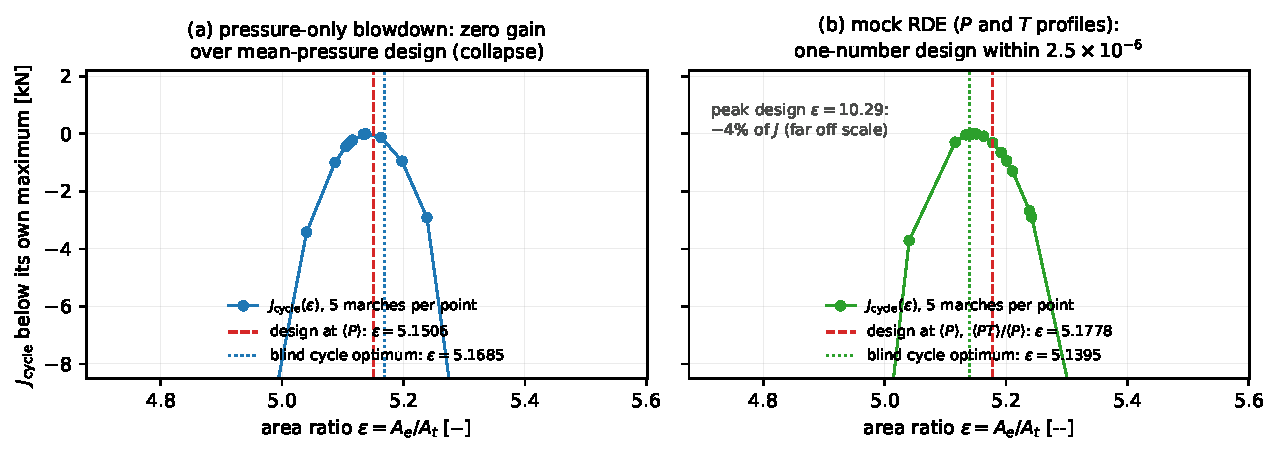
\includegraphics[width=\textwidth]{fig_cycle.pdf}
\caption{Lo strato di ciclo, misurato. Assi in entrambi i pannelli:
rapporto di espansione $\varepsilon$ [--] (area di uscita su area di
gola, la variabile di progetto) contro la spinta mediata sul ciclo
dell'Equazione~\eqref{eq:jcycle}, riportata come deficit sotto il
massimo della curva stessa, in kN (zero è il miglior progetto sulla
curva; il livello assoluto è $J_{\rm cycle} \approx 116$~MN). Ogni
punto costa cinque marce complete di ugello, una per fase; le linee
verticali segnano i progetti candidati. (a)~Svuotamento a sola
pressione: l'ottimo di ciclo trovato alla cieca
($\varepsilon = 5.1685$) cade sul classico progetto alla pressione
media ($\varepsilon = 5.1506$) entro la finestra derivata --- il
collasso a guadagno nullo, riprodotto da un motore cui non era mai
stato detto che dovesse accadere. (b)~RDE simulato, con pressione
\emph{e} temperatura variabili: l'ottimo alla cieca
($\varepsilon = 5.1395$) e il progetto a un solo numero allo stato
medio pesato sulla pressione ($\varepsilon = 5.1778$) differiscono
dello $0.74\%$ in $\varepsilon$ e di $2.5\times10^{-6}$ in $J$; il
progetto alla pressione di picco ($\varepsilon = 10.29$) perde il 4\%
e cade molto fuori scala. Si noti quanto sono piatte le curve vicino
ai loro picchi: la storia vive nelle ultime cifre, ed è per questo
che le soglie sono derivate anziché stimate a occhio.}
\label{fig:cycle}
\end{figure}

\section{Il compromesso mediato, su un misuratore}
\label{sec:votes}

\subsection{La domanda}

L'affermazione più citabile della teoria sugli ugelli per
RDE~\cite{theory} è la condizione di spigolo mediata: ``nessuna fase
soddisfa la propria condizione di spigolo; la media di ciclo sì''.
Si può misurare?

\subsection{Come funziona, per esteso}

Si richiami la condizione di spigolo della
Sezione~\ref{sec:corner}: l'affermazione esatta che la parete di un
ugello si ferma nel punto giusto, il cui termine dominante è lo
scarto fra la pressione che il gas raggiunge all'uscita e la
pressione ambiente in cui scarica. All'ottimo di ciclo ogni fase
$\xi$ esprime un \emph{voto} attraverso quello stesso misuratore: il
proprio scarto di pressione di uscita $R(\xi) = p_e(\xi) - p_a$. Una
fase con $R > 0$ lascia l'ugello ancora spingendo più forte
dell'ambiente --- \emph{sotto-espansa}, vota ``allungami''. Una fase
con $R < 0$ si è espansa sotto l'ambiente --- \emph{sovra-espansa},
vota ``accorciami''. L'affermazione è che l'ottimo non soddisfa
nessuna fase individualmente: è un compromesso mediato in cui la
media pesata con $\mu$ dei voti è nulla mentre nessun singolo voto
lo è.

Il misuratore legge i voti dalle esecuzioni di ciclo memorizzate, e
ogni soglia è derivata. La banda di equilibrio attorno allo zero
viene dalla curvatura dell'obiettivo stesso e dall'ampiezza della
finestra in cui l'ottimizzatore si è fermato --- quanto lontano
dallo zero la media potrebbe legittimamente trovarsi. Ogni voto di
fase deve poi individualmente superare quella banda; altrimenti
``nessuna fase soddisfa la propria condizione'' sarebbe
un'asserzione anziché una misura.

\subsection{Risultati di riferimento}

\textbf{8/8 PASS su entrambi i cicli}
(\carrier{validation/a1\_cycle\_corner.py}, un'analisi delle
esecuzioni di ciclo memorizzate --- 0.4~s). All'ottimo dell'RDE
simulato i voti delle cinque fasi vanno da $+7.9\times10^{5}$ fino a
$-5.1\times10^{5}$~Pa --- monotoni in fase, con esattamente un
cambio di segno, ciascuno individualmente 2.8--3.2$\times$ la banda
di equilibrio e 14--90$\times$ la media raggiunta --- mentre la loro
\emph{media} sta a zero entro la banda derivata. Sul progetto
sbagliato (alla pressione di picco) il misuratore si inchioda a
$-4.6\times10^{5}$~Pa: tutte le fasi sovra-espanse, nessun
compromesso. Un progetto sbagliato è visibile a colpo d'occhio.

\begin{figure}[htbp]
\centering
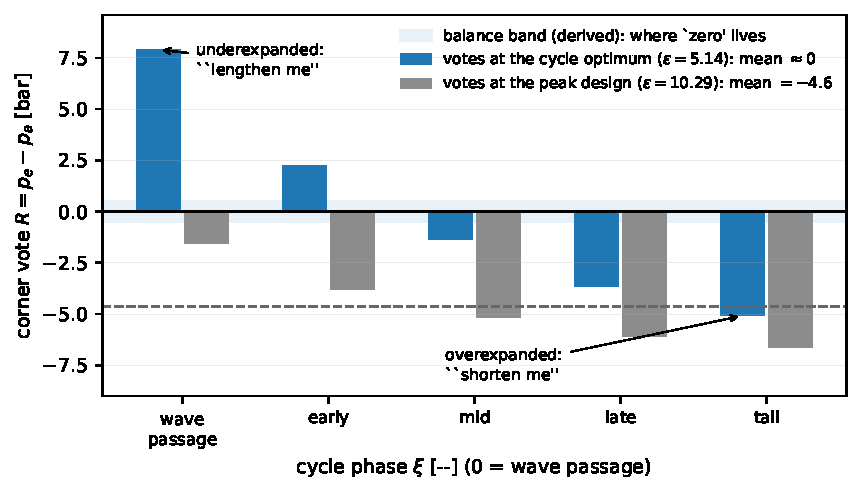
\includegraphics[width=0.85\textwidth]{fig_votes.pdf}
\caption{Il teorema su un quadrante. Asse orizzontale: fase di ciclo
$\xi$ [--], un giro dell'onda dal passaggio alla coda dello
svuotamento. Asse verticale: il voto di spigolo di ciascuna fase
$p_e - p_a$ [bar], la quantità di cui la sua pressione di uscita
supera (positivo: sotto-espansa, ``allungami'') o non raggiunge
(negativo: sovra-espansa, ``accorciami'') la pressione ambiente. Blu:
i voti all'ottimo di ciclo --- grandi e di entrambi i segni, eppure
la loro media (blu tratteggiato) sta dentro la banda ombreggiata di
equilibrio allo zero. È la condizione di spigolo mediata, misurata:
nessuna fase è individualmente soddisfatta, il ciclo sì. Grigio: gli
stessi voti sul progetto alla pressione di picco --- tutte le fasi
sovra-espanse, la media (grigio tratteggiato) molto sotto lo zero: un
progetto sbagliato, a colpo d'occhio.}
\label{fig:votes}
\end{figure}

\chapter{The plug march}
\label{ch:plug}

Every nozzle in this document so far has been a bell: a solid tube
that wraps the gas on all sides. This chapter builds the other kind.
A plug nozzle keeps solid metal only \emph{under} the flow and lets
the outside of the jet touch the atmosphere directly --- one change
that buys the nozzle the ability to adapt itself to its
surroundings, and costs the solver a boundary it has never had to
handle. The step adds that boundary, assembles a complete plug
march around it, and certifies the assembly against a flow whose
answer is known exactly on paper.

\section{The question}

The deepest results in the RDE nozzle theory are about plugs
(the corpus's plug theorem, its T4)~\cite{theory} --- in particular
about what a plug does when the chamber pressure swings over a
cycle, which is Chapter~\ref{ch:plugcycle}. None of them can
be tested until the engine can march a plug at all. So: what does
the solver need that it does not yet have, and can the new assembly
be checked against an exact answer rather than only against itself?

\section{How it works, in full}

\subsection{The topology, and the one new piece of physics}

A plug (or \emph{aerospike}) nozzle is a bell turned inside out. In
a bell the gas is enclosed by wall all the way to the exit. In a
plug the wall lies only below the flow --- a central body, the
\emph{spike} --- and above the flow there is nothing but the
surrounding atmosphere. The outer surface of the exhaust is
therefore a \emph{free jet edge}: a boundary of the gas that no
hardware holds in place.

That is the whole appeal of the shape. Because the outer boundary
is free, the jet widens or narrows on its own until its pressure
matches the atmosphere. A bell has one fixed exit area, so it is
correctly expanded at exactly one ambient pressure and wrong at
every other; a plug re-shapes its own jet as the ambient pressure
falls with altitude. That is the classical
\emph{altitude-compensation} argument for plugs
(Chapter~\ref{ch:nozzle}) --- and it is why plugs matter here for a
second reason: an RDE swings its chamber pressure every cycle,
which the nozzle feels the same way it feels a change of altitude.

The free edge is the one new piece of physics the solver must
learn. On a wall, the \emph{position} is known and the pressure
comes out as a result; on a free edge it is exactly the reverse.
The pressure is prescribed --- $p = p_a$, the ambient pressure,
because the atmosphere pushes back and nothing else does --- and
the \emph{position} is what gets solved. In the cell language of
Chapter~\ref{ch:moc}, the free-edge cell is fed by the previous
edge point (the edge is a \emph{streamline}: a line the flow runs
along and no gas crosses) and by the $C^{+}$ characteristic rising
from the interior point below it in its own column. The prescribed
pressure fixes the speed modulus $q_{p_a}$ through the gas tables,
so the two remaining unknowns are the new position and the turning
angle $\theta_4$, with
$(u,v) = q_{p_a}(\cos\theta_4, \sin\theta_4)$
(Figure~\ref{fig:freejet}). The assembly then mirrors the bell
march upside down: spike wall below (the inverse-wall cell of
Chapter~\ref{ch:wallinput}, mirrored to the $C^{-}$ family that a
bottom wall receives), free edge above, no axis~\cite{raospike}.

\begin{figure}[htbp]
\centering
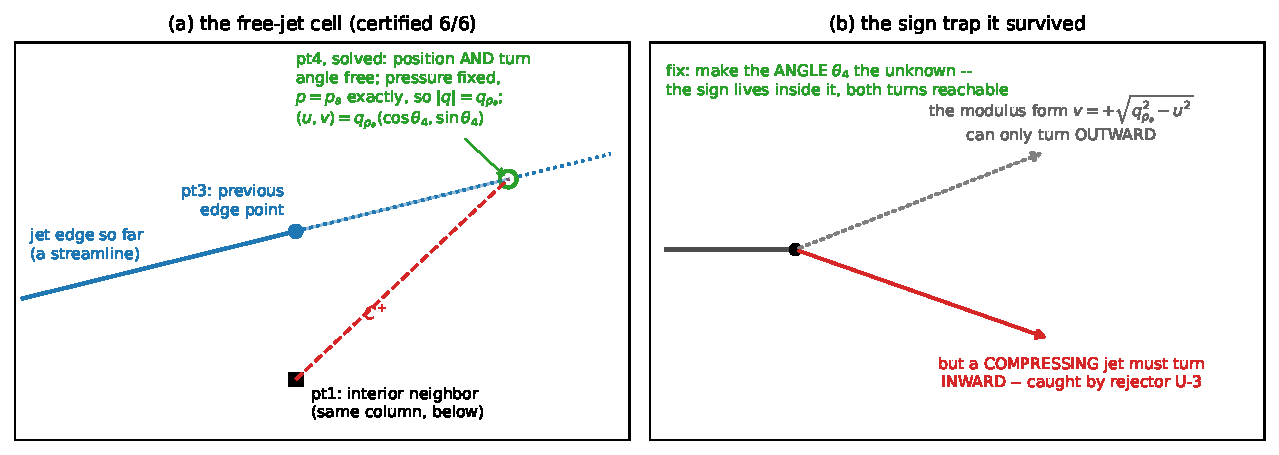
\includegraphics[width=0.95\textwidth]{fig_freejet.pdf}
\caption{The free-boundary cell, drawn in the physical plane:
$x$ axial [m] against $y$ radial [m]. (a)~The new edge point pt4 is
built from two known states --- the previous edge point pt3, whose
flow direction sets the direction of the edge segment because the
edge is a streamline, and the interior neighbour pt1 in the same
column, which sends the $C^{+}$ characteristic. What to look at is
which quantity is held and which floats: the pressure is
\emph{imposed}, $p = p_a$ exactly, which fixes the speed modulus
$q_{p_a}$ through the tables, while the position $(x_4,y_4)$ and
the turning angle $\theta_4$ are solved. That inversion --- the
opposite of a wall cell, where position is given and pressure comes
out --- is what makes a plug a plug. (b)~The same cell with the
sign trap it survived on the way to certification: writing the
boundary condition as $v = +\sqrt{q_{p_a}^2-u^2}$ admits only
outward turns (Appendix~\ref{app:signtrap}).}
\label{fig:freejet}
\end{figure}

\subsection{Why the lip fan is constructed, not marched}

At the \emph{cowl lip} --- the sharp outer edge of the channel that
feeds the plug --- the gas leaves the internal duct and turns
around a corner into the open. A supersonic gas turning away from
itself expands through a \emph{Prandtl--Meyer fan}: a continuous
sheaf of straight rays, each carrying one intermediate state,
across which the flow accelerates, its pressure falls, and its
direction rotates smoothly from the incoming angle to the outgoing
one. When the corner is sharp, every ray starts from the same
geometric point and the fan is \emph{centered} on it. That point is
\emph{singular}: all the intermediate states coexist there at once,
so the flow has no single value at the lip and its gradients are
infinite (Figure~\ref{fig:fansing}).

This violates exactly the assumptions an ordinary cell rests on. A
cell whose segment spans the fan closes its compatibility relation
with a midpoint average of two states that differ by the whole turn
--- an order-one error, not a second-order one --- and near the lip
all the $C^{-}$ characteristics meet at one point, so the position
crossing degenerates. Measured: a certification residual of
$8.9\times10^{9}$ when an early build tried exactly this.

The cure costs nothing, because a centered fan is self-similar: the
state on each ray depends only on the ray angle and is given
exactly by the Prandtl--Meyer function. So the corner is never
marched, it is \emph{constructed} --- seed the fan as data, then
resume ordinary cells between rays, where the flow is smooth again.
Brick 1 does precisely this at its sharp throat corner (the initial
expansion fan); the oracle below goes one step further and places
the start line downstream of the lip with the exact fan field
written on it, so the singular point lives in the data and never
inside a cell.

\begin{figure}[htbp]
\centering
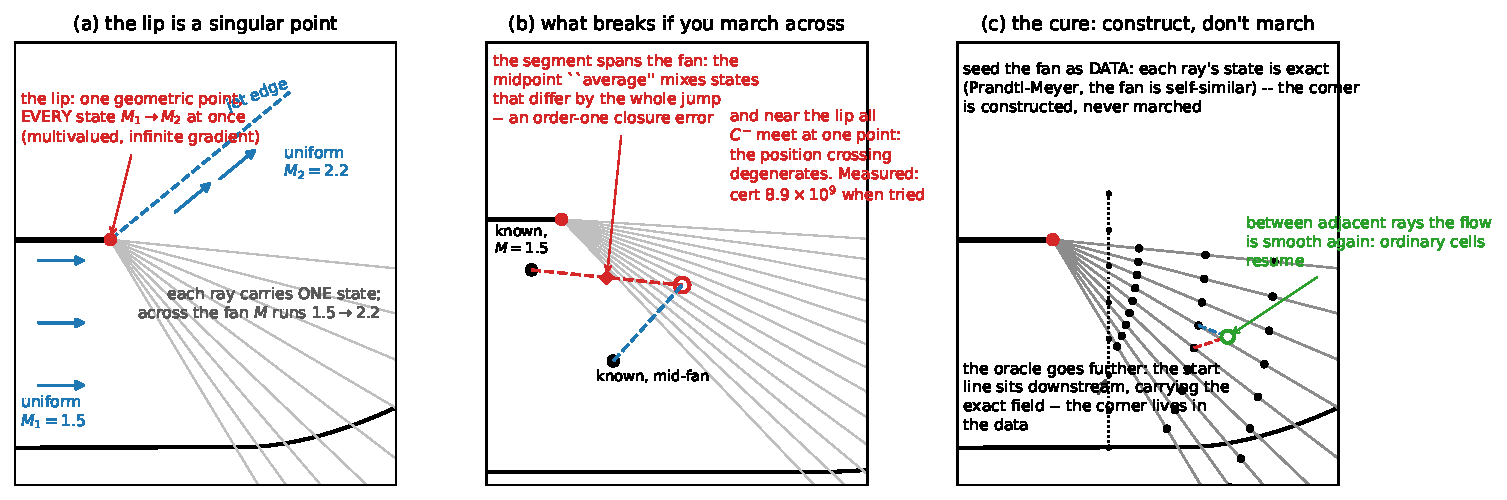
\includegraphics[width=\textwidth]{fig_fan_singularity.pdf}
\caption{Why the lip fan cannot be marched through. All panels are
the physical plane, $x$ [m] against $y$ [m]. (a)~The lip as a
singular point: a uniform stream at $M_1$ and a uniform stream at
$M_2$ meet across a centered fan whose every ray emanates from one
geometric point, so at the lip every state between $M_1$ and $M_2$
coexists and the gradient is infinite. (b)~An ordinary cell asked
to step across it: its segment spans the fan, so the midpoint
closure averages two states separated by the whole turn, and the
$C^{-}$ crossings degenerate as they converge on the lip ---
measured, a certification residual of $8.9\times10^{9}$. (c)~The
cure: each ray is seeded with its exact Prandtl--Meyer state and
ordinary cells resume between rays; the oracle puts the start line
downstream, carrying the exact field. What this proves is that the
singularity is handled by construction, not by refinement --- no
mesh is fine enough to march through a point where the solution is
multivalued.}
\label{fig:fansing}
\end{figure}

\subsection{The march: columns, growth at the edge, consumption at
the wall}

Each column is swept \emph{bottom-up}: first the wall point at the
prescribed station, then the interior points, each fed by the
$C^{+}$ from the point just solved below it and the $C^{-}$ from
its partner on the previous column, and finally the free-edge point
on top, fed from its own column (why it must be its own column is a
lesson the oracle taught: Appendix~\ref{app:edgeroot}).

The wall cell finds its foot --- the point on the previous column
where the characteristic arriving at the wall started --- by a
\emph{multi-column search}: it scans the whole previous column,
stepping further columns back if needed, for the segment whose data
brackets its arriving $C^{-}$ (the bracketing function is positive
at the previous wall point and decreases with row height, so the
first sign change marks the foot segment). This lets the march run
at fine prescribed stations with short compatibility chords; the
earlier scheme, which confined the foot to the first segment of the
adjacent column, had to stretch its columns and paid for it in
accuracy (Appendix~\ref{app:footbias}).

Row bookkeeping closes the topology, one characteristic at a time,
at both boundaries. At the \emph{edge}, each column's free-edge
point becomes a new top row: the widening jet gains one crossing
per column (the mirrored $j_2{+}{=}1$ of the bell march; what
happens without it is Appendix~\ref{app:pluglessons}, lesson 2).
At the \emph{wall}, rows are instead \emph{consumed}: the incoming
$C^{-}$ family terminates on a solid wall, so any previous-column
rows lying below the new wall point's foot have already met the
wall between stations and must not be prolonged --- the new
column's interiors are partnered with the previous rows \emph{from
the foot up}, re-indexed. Prolonging them was the last defect the
oracle caught: the terminated characteristics kept marching as
ghost rows below the spike --- for such a row the only crossing
Newton can still find is the backward one, a valid root of the
equations on the wrong branch --- and the mass check exposed the
ghost limb at $+9\%$. With consumption, mass closes to 0.026\%.

\subsection{The oracle}

The march is certified against a flow whose \emph{entire field} is
known in closed form, so the marched answer can be compared with
the truth rather than with itself. The flow is a planar corner jet:
uniform $M_1 = 1.5$, a centered fan at the lip, uniform $M_2 = 2.2$
turned by $\Delta\nu = 23.9^{\circ}$, with the ambient set to
$p_a = p(M_2)$. The prescribed spike is the exact streamline of
that field, obtained by fine-step RK4 integration --- an
independent reference, not another method-of-characteristics run
--- and the start line carries the exact field on a vertical cut.

The marched solution must then reproduce four things, each within a
tolerance derived from the scheme's own convergence order rather
than chosen by hand (Chapter~\ref{ch:method}): the edge's
asymptotic angle and speed (P-1), the wall pressure distribution
station by station (P-2), mass conservation through the final
column (P-3), and a \emph{momentum balance} (P-4). The last one is
worth spelling out. Draw a closed \emph{control surface} around the
gas --- an imaginary boundary whose faces are the start line, the
final column, the spike surface and the free edge --- and require
that the momentum flowing out equals the momentum flowing in plus
the push the pressures exert on the faces, every pressure measured
relative to ambient. On the free edge the pressure \emph{is}
ambient, so measured that way the free face pushes exactly zero:
the plug's defining property, here tested rather than assumed.
Alongside these, a deliberately corrupted ambient (R-1) must leave
the bands --- a check that the checks can fail. Every cell is
Newton-certified.

\subsection{The axisymmetric stage}

For the axisymmetric plug on the real-gas tables no closed form
exists, so that stage certifies by \emph{internal} closures ---
conservation laws the solution must satisfy whatever the answer is.
The start-line data is a tables-consistent corner fan
($\mathrm{d}\theta = \sqrt{M^2-1}\,\mathrm{d}q/q$ integrated on the
tables' own $M(q)$), the prescribed spike is a streamline of that
data, and the checks are: Newton certification (A-1); mass
conservation with the $2\pi y$ flux weight of an axisymmetric ring
(A-2); the same ambient-gauge momentum balance (A-3); a
\emph{source-alive} control --- the same data marched with the
axisymmetric source term switched off ($\delta = 0$, planar) must
differ by more than the axisymmetric pair's own tolerance band,
which guards against an axisymmetric mode that is silently running
planar (A-4); and a corrupted-spike rejector (A-5).

\section{What was built}

\carrier{validation/a1\_freejet\_unit.py}: the free-jet cell alone,
against unit known answers. \carrier{validation/a1\_plug\_march.py}:
the assembly --- bottom-up columns at prescribed stations, the
mirrored inverse-wall cell, the multi-column foot search, row
growth at the edge and row consumption at the wall --- plus the
conservation instruments (\code{col\_fluxes},
\code{wall\_push\_poly}), the closed-form oracle with its rejector
(\code{STAGE=oracle}), and the axisymmetric internal-closure stage
(\code{STAGE=axi}).

\section{Results of record}

\textbf{The free-jet cell: 6/6 PASS.} A uniform jet already at
ambient pressure is an exact fixed point; a turned jet is preserved
exactly in planar flow --- in axisymmetric flow the source term
legitimately changes a turned uniform state, a physics point the
first test tripped over; a compressing edge turns inward; and the
Prandtl--Meyer corner known answer lands at machine precision ---
edge speed vs.\ closed form $1.9\times10^{-9}$, edge angle equal to
the exact turn angle to $1.9\times10^{-16}$.

\textbf{The assembly vs the oracle: 6/6 PASS} (66~s, stations
41/81, start rows 21/41). Every cell Newton-certified --- worst
residual 0.019 (coarse, 1253 cells) and 0.017 (fine, 4870 cells) of
the allowed tolerance. P-1: the marched edge's tail angle is
0.41809 vs.\ the exact $\Delta\nu = 0.41777$ --- $|d| =
3.2\times10^{-4}$ against a band of $4.5\times10^{-3}$, with the
edge speed equal to the closed form to all printed digits. P-2:
98\% of wall stations inside the derived band, maximum deviation
$9.8\times10^{-3}\,p_a$. P-3: mass through the final column 8869.98
vs.\ start-line 8867.65 --- $|d| = 2.33$ (0.026\%) against a band
of 26. P-4: momentum closure $6.9\times10^{3}$ on
$F_{\rm in} = 2.0\times10^{7}$ ($3.4\times10^{-4}$ relative; band
$7.2\times10^{4}$; coarse/fine ratio 3.6, confirming the scheme's
second order), with the free edge contributing zero by
construction. R-1: a 1\% corruption of the ambient moves the edge
angle $20\times$ outside the P-1 band --- rejected.
Figure~\ref{fig:plug} shows the certified march; the road here ---
four structural lessons, each measured --- is
Appendix~\ref{app:pluglessons}.

\textbf{The axisymmetric stage: 5/5 PASS} (39~s, stations 33/65,
start rows 17/33, NASA real-gas tables, tables-fan turn
0.4395~rad). A-1: all cells Newton-certified, worst residuals
0.017/0.022. A-2: mass with the $2\pi y$ weight, $|d| = 505$ on
$1.085\times10^{5}$ (0.47\%) against a band of 986. A-3: momentum
closure $-2.4\times10^{6}$ on $F_{\rm in} = 2.4\times10^{8}$
($1.0\times10^{-2}$ relative, inside its band). A-4: the
axisymmetric source is alive --- the wall speed at the last station
differs from the planar run by 156~m/s, $9\times$ the band. A-5: a
corrupted spike slope breaks the momentum closure at $5\times$ the
band --- rejected.

\begin{figure}[htbp]
\centering
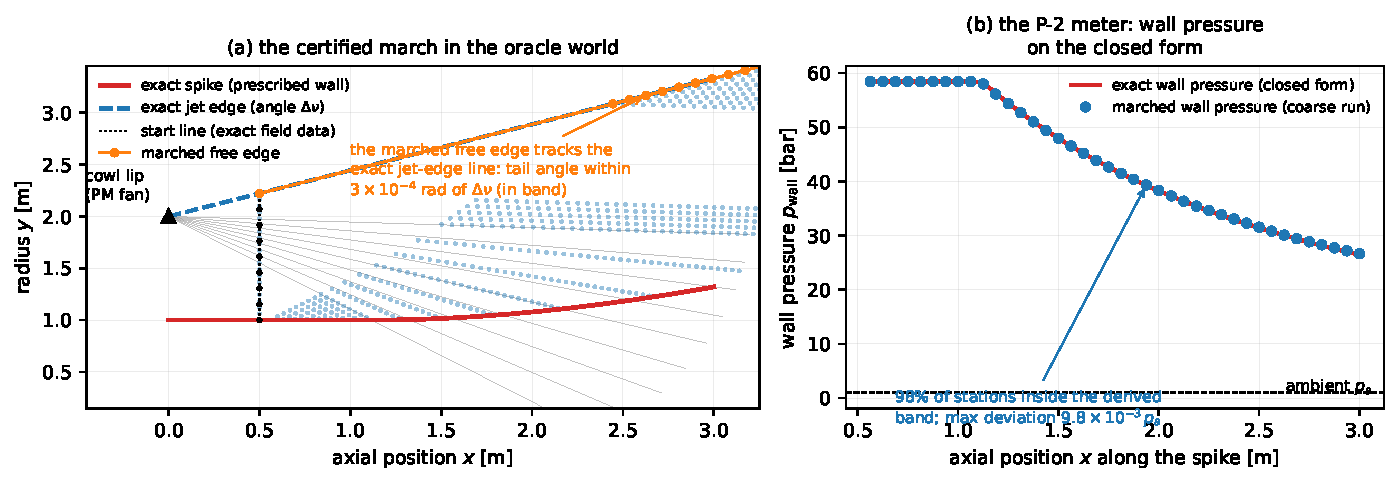
\includegraphics[width=\textwidth]{fig_plug.pdf}
\caption{The certified march against the closed-form oracle.
(a)~The physical plane, $x$ [m] against $y$ [m]: the exact world
--- spike (red), exact jet edge (blue dashed), lip fan rays (grey),
start line (dotted) --- overlaid with the marched characteristic
mesh (light dots) and the marched free edge (orange). Look at how
the orange edge tracks the blue line: told only the pressure on
that surface, the solver found where the surface is. (b)~Wall
pressure along the spike, $x$ [m] against $p_w$ [bar]: marched
values against the closed form, with the derived tolerance band ---
98\% of stations inside it, worst deviation
$9.8\times10^{-3}\,p_a$. The two panels together are the
certificate: the free surface and the solid surface are both right.
Compare with the state before the fixes,
Figure~\ref{fig:plugbefore}.}
\label{fig:plug}
\end{figure}

\chapter{Il plug troncato sotto il ciclo}
\label{ch:plugcycle}

Il Capitolo~\ref{ch:plug} sa marciare un plug a una condizione di
camera. Un motore a detonazione rotante non offre mai una sola
condizione: la sua onda di detonazione spazza l'anello e una sezione
fissa vede la pressione di camera salire di colpo e svuotarsi,
ancora e ancora. Questo capitolo taglia corta la spina --- i plug
reali sono sempre troncati, perché la coda lunga e sottile pesa
moltissimo e produce quasi nessuna spinta --- e si chiede dove
tagliare quando la pressione di camera oscilla in quel modo. La
risposta non risulta essere ``progettare per la condizione media'', e
la differenza è misurabile.

\section{La domanda}

Due tipi di ugello si comportano in modo opposto su un ciclo. La
campana fissa \emph{media}: il suo ottimo di ciclo è il progetto per
la singola condizione di pressione media, che il motore ha
certificato nel Capitolo~\ref{ch:cycle}. Il plug completo invece
\emph{massimizza}: l'ottimo di ogni fase contiene ogni plug più
lungo, quindi il plug ideale è dimensionato sulla fase più forte. Il
plug \emph{troncato} è il punto in cui entrambi i meccanismi
falliscono insieme --- ``il primo problema di forma genuinamente
mediato''~\cite{theory}. Il motore sa misurare tutte e tre le
affermazioni: l'ordinamento, la sua rottura e la condizione di
ottimalità mediata che la sostituisce?

\section{Come funziona, per esteso}

\subsection{Che cosa afferma la teoria, e che cosa assume}

Prima due termini. Una \emph{fase di ciclo} $\xi \in [0,1]$ indica
dove ci si trova nella storia di camera che si ripete --- $\xi$
vicino al passaggio dell'onda è la parte ad alta pressione, $\xi$
vicino alla fine dello svuotamento è quella a bassa pressione
(Capitolo~\ref{ch:cycle}); la media di ciclo $\mu$ è la media di
tipo temporale su quelle fasi. E un plug è \emph{troncato} alla
lunghezza $l$ quando la spina è tagliata lì e chiusa con una base
piatta: l'intera questione di progetto è quale debba essere $l$.

Il risultato del corpus sui plug (la sua T-T4) è dimostrato sotto
una chiusura di \emph{adattamento ideale} --- un'assunzione fatta per
mantenere trattabile la dimostrazione: che a valle del punto di
piena espansione di ciascuna fase la pressione di parete si agganci
esattamente all'ambiente $p_a$, e a monte di esso scali con la
pressione di camera. Sotto quell'assunzione la spinta di una data
fase, $F(l;\xi)$, non decresce mai al prolungarsi del plug e diventa
esattamente costante oltre una lunghezza dipendente dalla fase
$l(\xi)$, con $l(\xi)$ maggiore per le fasi più forti. L'insieme
delle lunghezze ottimali di ciascuna fase è allora una semiretta
$[l(\xi), \infty)$, e queste semirette sono \emph{annidate}: quella
della fase più forte sta dentro tutte le altre. È l'annidamento a
far collassare il problema --- una sola lunghezza è ottimale per
tutti insieme, quindi la migliore media eguaglia la media dei
migliori,
$\max_\Sigma \int F\,\mathrm{d}\mu = \int \max F\,\mathrm{d}\mu$,
raggiunta dal plug non troncato dimensionato sulla fase di picco.

L'avvertenza di finezza allegata a quel teorema dice che cosa
distrugge l'annidamento: un limite sulla lunghezza, un modello di
pressione di base o un adattamento non ideale. Perso l'annidamento,
l'uguaglianza diventa una disuguaglianza stretta,
$\max\int < \int\max$, e l'ottimo soddisfa invece una
\emph{condizione di spigolo mediata} sul piano di troncamento --- i
voti di pressione di parete per fase devono lì bilanciarsi nella
media di ciclo. Ciò che il motore aggiunge è precisamente la
quantità che la chiusura elimina per ipotesi: la pressione di parete
realmente marciata non si aggancia. A valle dell'adattamento va
sotto e sopra $p_a$, e l'ampiezza di quello scostamento \emph{è} la
rottura dell'adattamento, misurabile fase per fase.

\subsection{Mediare il problema non è mediare la condizione}
\label{sec:avgnotavg}

La media di ciclo $\mu$ è una media di tipo temporale sulle fasi, ed
è tentante concluderne che la ``condizione di spigolo mediata su
$\mu$'' sia solo il progetto alla pressione media travestito. Non lo
è, e la distinzione è l'intero contenuto della dicotomia. Il
\emph{progetto alla pressione media} significa: costruire il singolo
flusso stazionario dello \emph{stato} mediato --- la fase la cui
pressione di camera è $\bar P_0$ --- e ottimizzare quell'unico
flusso. Per la campana fissa questo è legittimo, perché il flusso e
la spinta della campana sono \emph{lineari} nella pressione di fase:
la legge di scala (Lemma~A) dice che l'intero campo scala con $P_0$
su una geometria fissa, con l'ambiente che entra solo in modo
additivo attraverso il gauge di pressione. Per un problema lineare la
media delle soluzioni è la soluzione della media --- mediare-poi-
risolvere equivale a risolvere-poi-mediare. È esattamente per questo
che la campana collassa.

La \emph{condizione di spigolo mediata} invece risolve ogni fase come
il \emph{proprio} flusso non lineare, lascia che ciascuna esprima il
proprio voto $p_w(l^{*};\xi) - p_a$ sul piano di troncamento ---
positivo significa che quella fase sta ancora spingendo lì e vuole
più plug, negativo che viene trascinata e ne vuole meno --- e media
la \emph{condizione di ottimalità}:
$\int (p_w(l^{*};\xi) - p_a)\,\mathrm{d}\mu = 0$. Le due coincidono
solo se l'applicazione da fase a voto è affine --- e il plug rompe
quell'affinità attraverso il suo bordo libero: l'ambiente è
\emph{condiviso e fisso}, non scala con la fase, quindi la pressione
di parete di ogni fase satura verso lo \emph{stesso} $p_a$ nel
\emph{proprio} punto di adattamento. La media dei voti non è il voto
alla media. La suite qui sotto misura la differenza direttamente: il
progetto alla pressione media dà $l = 1.280$~m, la condizione mediata
colloca l'ottimo a $l^{*} = 2.103$~m --- tutt'altro luogo. In una
riga: il risultato della campana media il \emph{problema}; quello del
plug media la \emph{condizione}, e la media commuta solo con i
problemi lineari.

\subsection{Una marcia per fase copre ogni troncamento}

In flusso supersonico le perturbazioni non possono risalire la
corrente: ciò che accade in un punto è fissato interamente da una
regione limitata alle sue spalle, il suo \emph{dominio di
dipendenza}. Su una spina \emph{fissa}, troncare a $l$ rimuove
parete solo a valle di $l$, quindi nulla a $x < l$ può sentire il
taglio. Una sola marcia a spina completa per fase produce dunque in
forma chiusa l'intera famiglia dei troncamenti,
\begin{equation}
J(l;\xi) \;=\; F_{\rm in}(\xi)
\;+\; \int_{x_0}^{l} \left(p_w(x;\xi) - p_a\right)
\,2\pi y_w\,(-\mathrm{d}y_w),
\label{eq:trunc}
\end{equation}
dove ogni pressione è misurata rispetto all'ambiente, così il bordo
libero contribuisce zero (la pressione su di esso \emph{è} $p_a$) e
anche un piano di base a $p_b = p_a$ contribuisce zero. Derivando in
$l$ si ottiene la condizione marginale $\mathrm{d}J/\mathrm{d}l = 0$,
cioè $p_w(l) = p_a$ --- la condizione di spigolo del plug sul piano
di troncamento: estendere il plug esattamente fin dove la sua parete
sta ancora spingendo più forte dell'atmosfera. La sua media di ciclo
sulle fasi è la condizione di spigolo mediata di cui sopra. Lo studio
dei troncamenti a cinque fasi costa perciò cinque marce, e ogni
verifica qui sotto legge le curve di pressione di parete
memorizzate.

\subsection{Il mondo}

Assialsimmetrico, tabelle NASA di gas reale, un unico pezzo di
hardware fisso marciato da tutte le fasi. Labbro del cowl in
$(0, 2)$; il flusso anulare arriva a $M_i = 1.2$ diretto verso
l'asse ($\theta_i = -25^{\circ}$); il ventaglio di labbro ---
l'espansione di spigolo del Capitolo~\ref{ch:plug}, costruita per
ogni fase e coerente con le tabelle --- lo espande fino all'ambiente
condiviso. L'ambiente è posto in modo che la rotazione del ventaglio
sia circa $|\theta_i|$, cioè che il flusso esca all'incirca in
direzione assiale ($\theta_E \approx 0$): la classica condizione di
progetto del plug, che rende la spina --- una linea di corrente del
campo del ventaglio della fase media --- genuinamente
\emph{discendente} verso l'asse. La linea iniziale pone lo stesso
profilo $(M,\theta)(y)$ per ogni fase con la termodinamica propria
di ciascuna fase: dati esatti da legge di scala per il ciclo a sola
pressione, e la posizione naturale ``stesso profilo di Mach
all'iniettore'' per il ciclo simulato. Ogni fase gira attraverso la
marcia del plug certificata del Capitolo~\ref{ch:plug} (parete
assegnata, ricerca multi-colonna del piede, contabilità delle
righe); il ciclo stesso è la costruzione certificata del
Capitolo~\ref{ch:cycle} (cinque fasi log-uniformi, rapporto di
pressione $PR = 10$, rapporto di temperatura simulato
$TR = 1.306$).

\section{Che cosa è stato costruito}

\carrier{validation/a1\_plug\_cycle.py}: il costruttore del mondo
(ventaglio per fase coerente con le tabelle, linea di corrente della
spina sul campo medio), i kit di marcia per fase con cache su disco,
la famiglia di troncamenti in forma chiusa~\eqref{eq:trunc} e due
stadi --- \code{t3} (ciclo a sola pressione: la legge di scala a
livello di parete e l'anti-collasso a livello di troncamento) e
\code{mock} (profili di $P$ e $T$: l'ordinamento degli ottimi per
fase, la rottura misurata dell'adattamento, i voti di spigolo
mediati, il divario stretto $\int\max > \max\int$, la penalità del
progetto di picco) --- più un rigettatore ad ambiente corrotto.

\section{Risultati di riferimento}

\textbf{Ciclo a sola pressione (l'anti-collasso del plug): 5/5
PASS.} Tutte le marce di fase certificate da Newton. La legge di
scala a livello di parete compare dal vivo esattamente dove deve e
soltanto lì: sulla parte di parete ancora schermata dall'ambiente ---
a monte del primo arrivo del bordo, $x < 0.81$, trovato tracciando
all'indietro la $C^{-}$ del bordo fino alla parete --- le pressioni
di parete scalate $p_w/P_0$ collassano su un'unica curva a meno di
$4.7\times10^{-15}$, lo zero di macchina. Oltre quella stazione il
collasso si rompe, e quella rottura \emph{è} il meccanismo di
adattamento, nettamente localizzato. I troncamenti misurano poi la
dicotomia: la lunghezza ottimale di ciclo $l^{*} = 2.103$ sta molto
\emph{sopra} il progetto alla pressione media ($l = 1.280$) e appena
sotto il progetto di picco ($l = 2.336$) --- il plug \emph{non}
media, si sposta verso il picco, trattenuto al di qua di esso solo
dalla reale rottura dell'adattamento. Gli ottimi per fase
$l(\xi) = 2.336, 2.061, 1.125, 1.047, 1.006$ crescono con la
pressione di fase: l'\emph{ordine} di annidamento del teorema del
plug, dal vivo.

\textbf{RDE simulato (profili di $P$ e $T$), la media genuina: 9/9
PASS.} Lo stesso ordinamento ricompare
($l(\xi) = 2.336 \ldots 1.012$). L'adattamento non ideale è
\emph{misurato}: ogni fase interna perde spinta oltre il proprio
$l(\xi)$ (perdite relative da $1.6\times10^{-4}$ a
$2.0\times10^{-3}$) --- l'aggancio ideale non vale nel flusso reale,
e quella perdita è esattamente la quantità che rompe l'annidamento
ideale. Di conseguenza la disuguaglianza stretta dell'avvertenza di
finezza è risolta:
$\int\max - \max\int = 1.07\times10^{4}$ N ($2.3\times10^{-4}$ di
$J$), oltre la sua banda derivata; la penalità per progettare al
picco è $2.2\times10^{-4}$ di $J$, anch'essa risolta. All'ottimo di
ciclo trovato alla cieca la condizione di spigolo mediata vale: la
media dei voti è $+1.8\times10^{4}$ Pa contro una banda di
equilibrio di $3.1\times10^{5}$, mentre i singoli voti raggiungono
$\pm1.4\times10^{6}$ --- e l'ottimo è un compromesso strettamente
interno (gli ottimi per fase si distribuiscono su 1.32 in $l$;
nessuna fase estrema possiede $l^{*}$). Un ambiente corrotto sposta
la media dei voti $2.3\times$ fuori dalla banda --- rigettato. La
strada per arrivarci --- due lezioni di posizione del problema e due
verifiche che la teoria stessa ha rigettato --- è
l'Appendice~\ref{app:plugcycleposing}.

\textbf{Una lezione misurata che è fisica nuova, non un difetto.} La
struttura puntuale dei voti della campana --- monotona in fase, con
esattamente un cambio di segno (Capitolo~\ref{ch:cycle}) --- \emph{non}
si trasferisce al plug. A valle dell'adattamento la pressione di
parete \emph{oscilla} attorno a $p_a$, perché il ventaglio di labbro
si riflette sul bordo libero e ricade sulla parete. I voti puntuali
campionano dunque un'oscillazione, e la fase di passaggio dell'onda
può votare negativo a una lunghezza inferiore al proprio ottimo.
Sopravvivono solo il bilancio mediato e la struttura di compromesso
--- che è esattamente, e soltanto, ciò che l'avvertenza di finezza
afferma.

\begin{figure}[htbp]
\centering
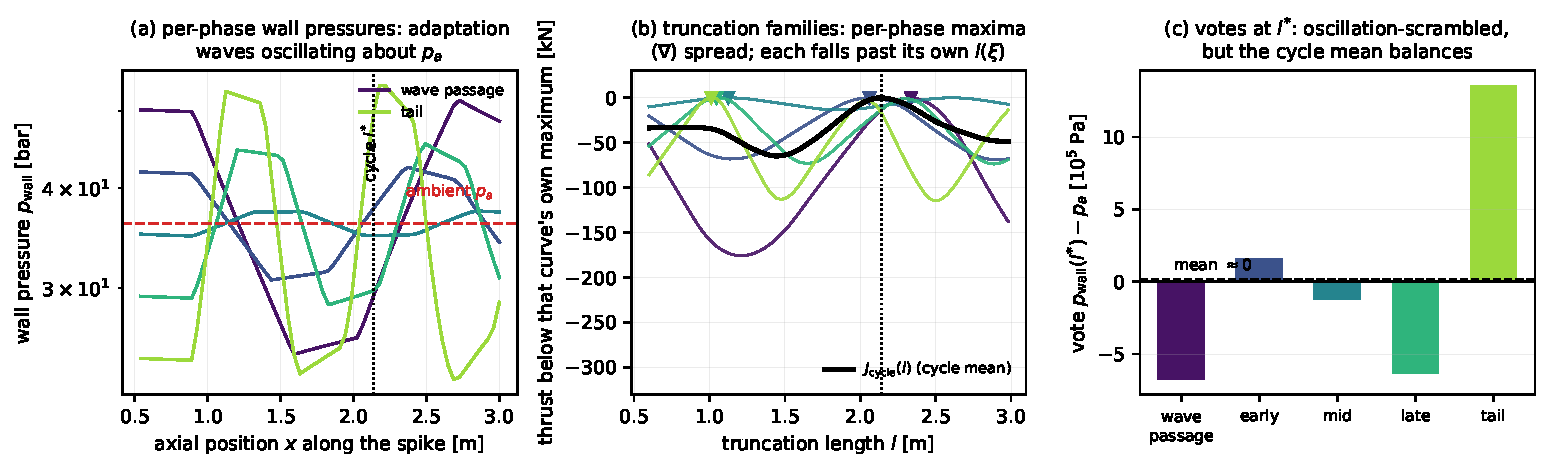
\includegraphics[width=\textwidth]{fig_plug_cycle.pdf}
\caption{Il plug troncato sotto il ciclo, misurato. (a)~Pressione di
parete lungo la spina fissa per ciascuna fase: $x$ [m] contro $p_w$
[bar], con l'ambiente condiviso $p_a$ disegnato come linea
orizzontale. Si guardi a valle della regione schermata: le curve non
si agganciano a $p_a$, vi \emph{oscillano} attorno --- il ventaglio
di labbro che si riflette sul bordo libero e torna sulla parete.
Quell'oscillazione è l'adattamento reale, non ideale, che la chiusura
della teoria elimina per ipotesi. (b)~Le famiglie di troncamento
dell'Equazione~\eqref{eq:trunc}: lunghezza di troncamento $l$ [m]
contro la deviazione di spinta di ciascuna curva dal proprio massimo,
$J(l;\xi) - \max_l J(l;\xi)$, in kN, così che zero significhi
``all'ottimo proprio di questa fase''. I massimi per fase ($\nabla$)
si distribuiscono da $l = 1.01$ a $2.34$~m nell'ordine della
pressione di fase, e ogni curva \emph{cala} oltre il proprio massimo
--- la rottura misurata dell'annidamento ideale, che le avrebbe
tenute piatte. La media di ciclo $J_{\rm cycle}(l)$ (nero) ha il
picco a un compromesso $l^{*}$ che nessuna singola fase possiede.
(c)~I voti a quell'ottimo: fase di ciclo $\xi$ [--] contro
$p_w(l^{*};\xi) - p_a$ [bar]. Sono scompaginati nell'ordine dei segni
dall'oscillazione di adattamento --- la struttura monotona dei voti
della campana non si trasferisce --- eppure la loro media di ciclo
(tratteggiata) si bilancia a zero dentro la banda derivata. È tutta
qui l'affermazione: non che qualche fase sia soddisfatta, ma che lo
sia la loro media.}
\label{fig:plugcycle}
\end{figure}

\chapter{Il gemello a campo intero del plug GENO}
\label{ch:genotwin}

Due programmi scritti in modo indipendente, in linguaggi diversi,
che si verificano a vicenda su un unico problema fisico sono un test
più forte di qualunque cosa ciascuno possa eseguire da solo: una
risposta condivisa non può venire da un errore condiviso. Questo
capitolo esegue quell'esperimento su un ugello a spina (aerospike)
--- uno la cui parete solida, la \emph{spina}, sta sotto lo scarico
mentre l'esterno del getto è delimitato da nient'altro che
l'atmosfera circostante. Il codice Fortran indipendente di progetto
GENO~\cite{geno} progetta una tale spina; il nostro solutore prende
quella forma come una comune parete assegnata, ricalcola l'intero
flusso attorno a essa, e i due campi di moto vengono confrontati
numero per numero. Il passo consegna la più forte verifica esterna
del programma --- e un risultato onesto.

\section{La domanda}

La sessione GENO a due vincoli (Capitolo~\ref{ch:status},
Sezione~\ref{sec:designinputs}) ha lasciato un residuo dichiarato:
il confronto a \emph{campo intero}. Non una manciata di grandezze
riassuntive, ma la nostra marcia del plug certificata eseguita sul
contorno di spina che il modulo RaoPlug di GENO ora produce in modo
pulito, confrontata campo contro campo --- pressione di parete
stazione per stazione, velocità nei punti interni di GENO, e massa e
spinta integrate. È la controparte per il plug della verifica fra
codici dell'ugello a campana del Capitolo~\ref{ch:referee}.

\section{Come funziona, per esteso}

\subsection{Che cosa occorre sapere prima}

Il solutore avanza un flusso supersonico lungo le due famiglie di
\emph{caratteristiche} --- le linee lungo cui una perturbazione può
viaggiare in flusso supersonico, inclinate dell'angolo di Mach da una
parte e dall'altra della direzione del flusso (Capitolo~\ref{ch:moc};
simboli nella Tabella~\ref{tab:notation}). Qui servono altre tre
parole.

Una \emph{linea iniziale} (o taglio di Cauchy, dal problema ai valori
iniziali che pone) è una linea tracciata attraverso il flusso sulla
quale lo stato completo --- posizione, velocità, pressione --- è
fornito come dato. Data una linea iniziale e le pareti, le equazioni
determinano tutto ciò che sta a valle di essa e nulla a monte. La
nostra è un taglio verticale attraverso il campo finito di GENO.

La \emph{linea dei valori iniziali} (IVL) è l'ultima caratteristica
della costruzione propria di GENO --- il bordo esterno della regione
che GENO calcola. Sotto di essa c'è il campo di progetto di GENO;
sopra, GENO non ha nulla da dire.

Il \emph{troncamento} compare qui in due sensi standard non
collegati, e il capitolo ha bisogno di entrambi: tagliare corta la
spina a una lunghezza finita (hardware), e l'errore che uno schema a
passo finito commette perché i suoi passi non sono infinitesimi
(numerica). Il risultato qui sotto riguarda il secondo.

\subsection{Due costruzioni indipendenti}

GENO costruisce la spina \emph{all'indietro}: ruota il ventaglio di
espansione al labbro del cowl a passi angolari fissi
($0.05^{\circ}$), integra una caratteristica per ogni membro del
ventaglio con le proprie celle, colloca ciascun punto di parete
richiedendo che la massa che scorre dentro quella caratteristica
eguagli la massa che la gola lascia passare (la terminazione di
massa, la N-65 di GENO) e taglia la spina nel punto $D$ in cui quel
bilancio è soddisfatto.

Il nostro motore non sa nulla di quella costruzione. È una marcia
assialsimmetrica generale --- celle interne, celle a parete assegnata
con la ricerca multi-colonna del piede, il bordo di getto libero,
ciascuna certificata nel Capitolo~\ref{ch:plug} --- e tratta il
contorno di GENO come una comune parete assegnata, marciando
\emph{in avanti} a partire da una linea iniziale. L'accordo è dunque
una prova sul problema continuo condiviso, non su codice condiviso.

\subsection{La posizione del problema: tutti i dati sono di GENO}

Non si assume nulla di analitico. Perfino il gas è identificato
\emph{dal campo di GENO}: il rapporto dei calori specifici
$\gamma = 5.34782609/4.34782609$ (la ricetta che il backend
termodinamico di GENO stesso implementa, un gas a calore specifico
costante), la costante del gas $R_g$ da $p/(\rho T)$ nei suoi punti
(dispersione $8.7\times10^{-9}$) e l'isentropica efficace del campo
stesso. Quest'ultima conta: il campo di GENO sta in realtà a una
pressione di camera $p_0 = 6.008172\times10^{6}$~Pa, \emph{non} al
nominale $6\times10^{6}$ --- uno scostamento uniforme della sua
costruzione, dispersione $1.1\times10^{-4}$ --- e porre il valore
nominale avrebbe fabbricato una differenza che non c'è.

La linea iniziale è un taglio verticale a $x_0 = 0.15$ attraverso le
caratteristiche di prima fase di GENO; ogni attraversamento è
interpolato sui punti propri di quella curva e verificato contro
un'interpolazione bidimensionale indipendente dello stesso campo, con
accordo a $10^{-5}$. La parete è il contorno di GENO, con pendenze
$\tan\theta_w$ misurate da esso (la sua tangenza è coerente a
$1.6\times10^{-5}$).

Sopra la linea dei valori iniziali giace una regione che GENO non
calcola, e la nostra marcia ha bisogno di qualcosa lì, quindi si pone
una striscia di getto libero, raccordata con continuità dallo stato
all'attraversamento della IVL allo stato sull'ultimo membro del
ventaglio. Non può contaminare il confronto --- un fatto sul flusso
supersonico, non una speranza, poiché ogni punto è influenzato solo
da ciò che sta a monte dentro il suo cono di dipendenza: ogni
caratteristica che arriva alla parete prima di $D$ lascia la linea
iniziale \emph{sotto} la IVL, e la IVL stessa atterra esattamente in
$D$, la fine della parete. È stato comunque verificato: sostituire
la striscia raccordata con una uniforme non cambia nulla sulla
parete.

\subsection{Soglie: dichiarate, con provenienza}

Ovunque altrove in questo programma la banda di superamento è
\emph{derivata}: lo stesso calcolo è eseguito a due risoluzioni, la
variazione misura l'errore proprio dello schema, e la banda è quella
variazione gonfiata da un fattore di sicurezza
(Capitolo~\ref{ch:method}). Qui i livelli sono invece
\emph{dichiarati} --- fissati in anticipo, con la loro provenienza
--- deliberatamente, per la ragione che è il risultato centrale di
questo passo qui sotto: la differenza misurata fra i due codici sta
\emph{sopra} ciò che il raffinamento di passo di ciascun codice
suggerisce, quindi una banda derivata dal raffinamento sarebbe il
metro sbagliato.

I livelli dichiarati vengono dall'accordo fra codici già stabilito
--- un integratore indipendente della curva di progetto, costruito
nella sessione a due vincoli, coincideva con GENO a tre o quattro
cifre significative --- rimisurato qui sul campo intero, con almeno
un fattore due di margine su ogni statistica: pressione di parete
$3\times10^{-3}$ (mediana misurata $1.9\times10^{-3}$), campo
assestato $q\ 10^{-3}$ / $\theta\ 1.5\times10^{-3}$ (95-esimo
percentile misurato $4.5\times10^{-4}$ / $5.3\times10^{-4}$),
integrali attraverso la frontiera condivisa $2.5\times10^{-3}$
(misurato $1.2\times10^{-3}$). Ciò che tiene onesti dei numeri
dichiarati sono i \emph{rigettatori} --- esecuzioni deliberatamente
corrotte che la suite deve far fallire (Capitolo~\ref{ch:method}):
dimostrano che lo strumento risolve difetti di un ordine di
grandezza superiori al divario che sta misurando. Una verifica
mantiene bande interamente derivate: l'identificazione del gas è
giudicata contro i pavimenti di autoconsistenza misurati di GENO
stesso (entalpia totale $2.0\times10^{-5}$, entropia
$4.7\times10^{-6}R$, pressione totale $1.1\times10^{-4}$).

\section{Che cosa è stato costruito}

\carrier{validation/a1\_geno\_plug\_twin.py}: l'estrattore di
riferimento (cartella di esecuzione GENO $\to$
\code{\_geno\_twin/ref.npz}: parete, linea dei valori iniziali, i
131{,}589 punti di campo di prima fase, identificazione del gas,
pavimenti), il costruttore del mondo della linea iniziale, la
quadratura di flusso calibrata --- lungo l'intera linea dei valori
iniziali di GENO riproduce la portata $\dot m$ stampata da GENO a
$2.4\times10^{-7}$ e la spinta $F$ a $2.3\times10^{-7}$, risolvendo
per strada una questione di definizione: la $F$ di GENO è
l'integrale di quantità di moto a pressione assoluta --- più le sei
verifiche di accordo G-1--G-6 e i due rigettatori R-1/R-2.

\section{Risultati di riferimento: 8/8 PASS}

G-1, il gas: le nostre tabelle riproducono pressione, temperatura e
densità di GENO nei suoi stessi punti a partire dalla sola velocità
locale, entro i pavimenti misurati di GENO (peggiore
$9.9\times10^{-5}$ in $p$). G-2: tutte le 25{,}034 celle certificate
da Newton a entrambe le risoluzioni. G-3, la parete: pressione entro
$3\times10^{-3}$ nel 100\% delle stazioni (mediana
$1.9\times10^{-3}$, peggiore $2.5\times10^{-3}$). G-4, l'interno:
superato il transitorio iniziale, il 97.7\% dei punti propri di GENO
concorda entro ($q\ 10^{-3}$, $\theta\ 1.5\times10^{-3}$); mediane
$3.8\times10^{-4}$ e $7.9\times10^{-5}$. G-5/G-6: massa e spinta
attraverso il tratto condiviso della linea dei valori iniziali
concordano a $1.2\times10^{-3}$ e $1.1\times10^{-3}$. Entrambi i
rigettatori scattano: un gas falsificato dell'$1\%$
($\gamma\times1.01$) fa crollare l'accordo di parete al 31\% delle
stazioni, un contorno scalato di $\times1.005$ lo fa crollare
allo 0\%.

\begin{figure}[htbp]
\centering
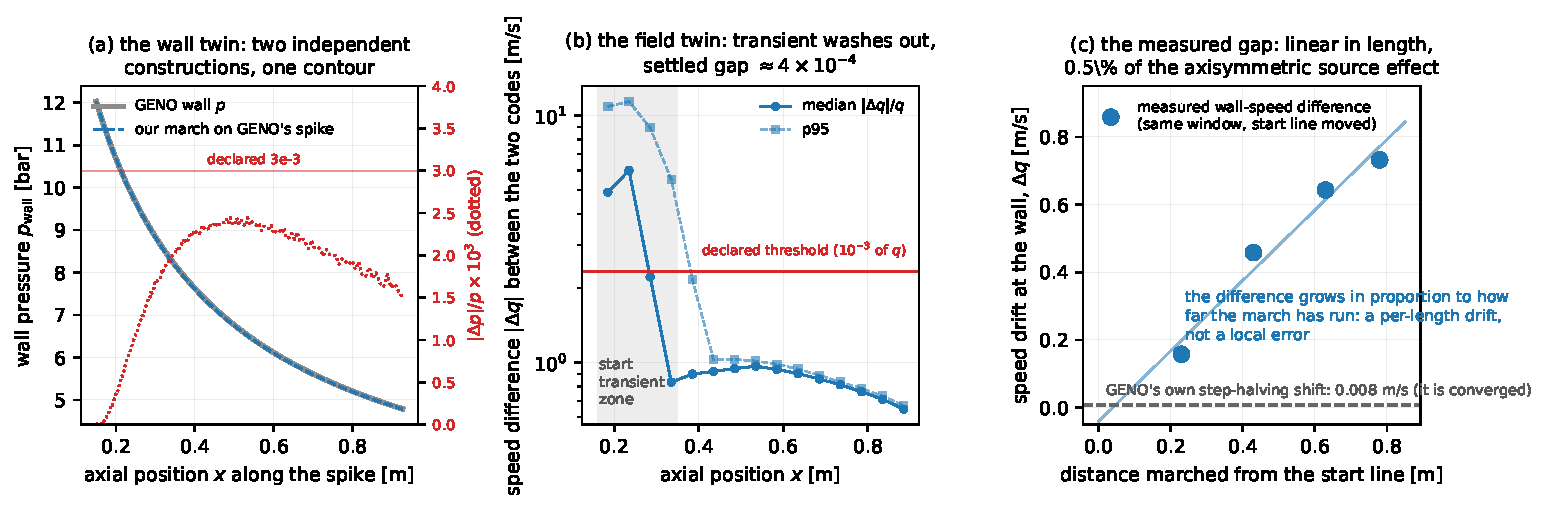
\includegraphics[width=\textwidth]{fig_geno_twin.pdf}
\caption{Il gemello a campo intero del plug GENO. (a)~Pressione di
parete lungo la spina: coordinata assiale $x$ [m] in orizzontale,
pressione sulla superficie della spina [bar] in verticale. La parete
propria di GENO (continua) e la nostra marcia in avanti sullo stesso
contorno (tratteggiata) si sovrappongono; la deviazione relativa
(punteggiata, asse destro, in unità di $10^{-3}$) resta sotto il
$3\times10^{-3}$ dichiarato in ogni stazione --- due codici, un
contorno, tre o quattro cifre. (b)~Lo stesso confronto dentro il
flusso: nei punti di campo propri di GENO, la differenza di modulo
della velocità fra i due codici, $|\Delta q|$ [m/s], contro $x$ [m]
(mediana e 95-esimo percentile per banda). Si guardi l'estremo
sinistro: il transitorio iniziale --- la nostra marcia che ingerisce
una linea iniziale tracciata attraverso la forte curvatura del flusso
vicino al labbro --- si esaurisce entro $x\approx0.35$~m, lasciando
un divario assestato di circa $4\times10^{-4}$ della velocità locale.
(c)~Che cosa sia quel divario assestato: la lunghezza effettivamente
marciata [m], variata spostando la linea iniziale, contro la
differenza di velocità che ne risulta alla parete $\Delta q$ [m/s]. I
punti cadono su una retta per l'origine ($\approx4\times10^{-4}$ di
$q$ per unità di lunghezza), mentre dimezzare i passi propri di GENO
sposta la parete di GENO di soli $3.5\times10^{-6}$ --- quindi non è
un errore locale in nessuno dei due codici ma una lenta deriva che si
accumula con la distanza marciata fra due solutori individualmente
convergenti, pari allo $0.5\%$ del contributo proprio del termine
sorgente assialsimmetrico.}
\label{fig:genotwin}
\end{figure}

\section{Il risultato: un divario fra codici misurato e con
attribuzione aperta}
\label{sec:twingap}

Il gemello certifica un accordo di tre-quattro cifre --- e la
differenza residua è essa stessa un risultato caratterizzato, non un
avanzo. Ha due parti. Vicino alla linea iniziale, un transitorio: a
quote intermedie l'angolo del flusso differisce fino a
$1.1\times10^{-2}$~rad, decadendo entro $x \approx 0.35$, invariato
al cambiare della risoluzione e mobile allo spostarsi della linea
iniziale --- la firma dell'ingestione di una linea iniziale
tracciata attraverso la forte curvatura del flusso vicino al labbro.
Si esaurisce. Ciò che resta è una \emph{deriva uniforme} assestata:
la nostra velocità corre $+4\times10^{-4}$ relativi più alta
sull'intera colonna, e quell'eccesso cresce linearmente con la
distanza marciata (Figura~\ref{fig:genotwin}c).

L'indagine ha escluso, per misura, ogni causa accessibile.
\emph{Il gas}: i due lati sono analiticamente equivalenti a circa
$10^{-8}$. \emph{La geometria della parete e la sua tangenza}:
$1.6\times10^{-5}$. \emph{I dati della linea iniziale}: concordi a
$10^{-5}$ per due vie di interpolazione indipendenti; raffinare la
risoluzione della poligonale da $10^{-4}$ a $5\times10^{-6}$ lascia
la deriva invariata. \emph{La striscia sopra la linea dei valori
iniziali}: sostituire il raccordo con uno stato uniforme non cambia
nulla, e il cono di dipendenza le vieta comunque di raggiungere la
parete. \emph{La discretizzazione di GENO}: una compilazione
diagnostica di GENO con il passo del ventaglio \emph{e} il passo
della curva entrambi dimezzati ha spostato la parete di GENO di
$3.5\times10^{-6}$, quindi GENO è convergente in passo (i sorgenti
sono poi stati ripristinati e il binario restaurato, con verifica
md5). \emph{La nostra risoluzione}: dimezzare ciascuno dei nostri due
conteggi di passo sposta la deviazione di meno del 10\% di sé
stessa.

Entrambi i campi soddisfano le stesse relazioni trapezoidali di
marcia a $10^{-8}$--$10^{-9}$ (un audit dei residui eseguito su
\emph{entrambe} le maglie). Ciò dimostra che i due sistemi discreti
sono algebricamente equivalenti --- e dimostra anche che un tale
audit è \emph{tautologico} come verifica di accuratezza: ogni codice
risolve esattamente le proprie relazioni, quindi un audit dei residui
non può mai vedere una distorsione che si accumula lentamente. Vale
la pena dirlo chiaramente, perché sembra una verifica forte e non lo
è. Infine, una marcia di controllo con il termine sorgente
assialsimmetrico spento dimensiona la deriva: è lo $0.5\%$ di ciò che
quel termine contribuisce alla velocità di parete (che è a sua volta
il $-5.4\%$ di $q$).

L'attribuzione resta onestamente \emph{aperta}. I meccanismi
candidati vivono precisamente dove il raffinamento non varia nulla
--- dal lato di GENO la contabilità della re-interpolazione durante
la sua marcia all'indietro, dal nostro l'interpolazione lungo la
corda trovata dalla ricerca del piede --- e dall'esterno, a questo
livello, non sono distinguibili. La domanda di competenza del
proprietario è depositata presso GENO. Per questo programma la
conseguenza operativa è quella già adottata: i confronti fra codici
con GENO portano il livello di accordo misurato di tre-quattro cifre
--- molto sopra l'errore di troncamento di entrambi i codici, molto
sotto qualunque cosa cui i gradienti dell'ottimizzatore siano
sensibili --- e i rigettatori tengono onesto lo strumento a quel
livello.

\chapter{Swirl a vortice libero}
\label{ch:swirl}

Tutto quanto precede ha assunto che il gas si muova in un piano
contenente l'asse: in avanti e verso l'esterno, mai attorno. Un
motore a detonazione rotante (RDE) --- un combustore in cui un'onda
di detonazione corre di continuo attorno a una camera anulare --- non
è così accomodante: il suo scarico esce \emph{ruotando}. Questo
capitolo aggiunge quella rotazione al solutore nell'unica forma che
non costa nuove ipotesi, mostra per dimostrazione e per misura che
l'intera macchina certificata le sopravvive, e dichiara con chiarezza
che cosa l'estensione modella e che cosa no.

\section{La domanda}

Poiché l'onda di detonazione spazza la camera, trascina con sé il
gas: lo scarico porta una \emph{velocità azimutale} $w$ --- la
componente di velocità che gira \emph{attorno} all'asse,
perpendicolare al piano passante per l'asse in cui il solutore lavora
(quel piano si chiama piano \emph{meridiano}, e $q_m$ indica la
velocità in esso). Il corpus della teoria garantisce (la sua
affermazione N6-2) che per un particolare profilo di swirl --- il
\emph{vortice libero} --- l'intera struttura della marcia certificata
sopravvive intatta, e che qualunque cosa oltre esso è una classe di
flusso che questo metodo non può rappresentare affatto, e che
appartiene alla linea dell'aggiunto CFD.

Un vortice libero è la rotazione dello scarico di una vasca lontano
dal suo nucleo: il prodotto del raggio per la velocità azimutale,
$\Gamma = y\,w$, è \emph{uno e lo stesso numero ovunque nel flusso}.
Quel prodotto si chiama \emph{circolazione}; misura quanto il gas
gira attorno all'asse e fisicamente è il momento angolare per unità
di massa. Lo swirl è dunque più veloce vicino all'asse e si spegne
verso l'esterno, ed è fissato da un solo scalare $\Gamma$.

La domanda di questo capitolo: il motore sa portare lo swirl, con la
garanzia \emph{misurata} anziché assunta --- e con lo swirl spento
($\Gamma \to 0$) che recupera esattamente la marcia certificata senza
swirl?

\section{Come funziona, per esteso}

\subsection{Perché il vortice libero è l'unica estensione gratuita}

Tre fatti esatti rendono speciale il vortice libero.

Primo, l'equazione della quantità di moto attorno all'asse dice che
$y\,w$ è trasportato invariato lungo ciascuna linea di corrente. Se è
una sola costante \emph{ovunque}, quell'equazione è soddisfatta
identicamente e $w = \Gamma/y$ è noto dalla sola posizione ---
nessuna nuova incognita entra nella marcia.

Secondo, il flusso resta \emph{irrotazionale}: le particelle di
fluido vengono trasportate e deformate, ma non ruotano attorno al
proprio centro. È questa la proprietà su cui posa l'intero solutore
--- è ciò che rende il flusso descrivibile con le due famiglie
caratteristiche del Capitolo~\ref{ch:moc}; un flusso le cui
particelle ruotano si dice \emph{rotazionale}, e per esso il metodo
delle caratteristiche non è più applicabile. È esattamente ciò che
sta oltre il vortice libero. Il teorema di Crocco, che lega la
vorticità ai gradienti di entalpia totale ed entropia, lascia
possibile solo una componente azimutale quando entrambe sono
uniformi, e la condizione $V \times \omega = 0$ costringe poi anche
quella ad annullarsi. Il flusso meridiano resta dunque irrotazionale,
e la struttura certificata a due caratteristiche non è qui
un'approssimazione ma è esatta.

Terzo, svolgendo le equazioni della gasdinamica con $w = \Gamma/y$ si
vede che il problema meridiano cambia in esattamente due punti e in
nessun altro:
\begin{itemize}[itemsep=1pt]
\item \textbf{lo stato}: l'energia cinetica della rotazione entra nel
  bilancio energetico, $h = h_0 - q_m^2/2 - \Gamma^2/(2y^2)$, quindi
  lo stato termodinamico dipende ora dal raggio $y$ oltre che dalla
  velocità meridiana $q_m$;
\item \textbf{la sorgente}: un gas che ruota dev'essere trattenuto da
  un gradiente di pressione diretto verso l'interno, e quel
  contributo centrifugo si somma al termine che il flusso
  assialsimmetrico già porta --- il \emph{termine sorgente
  assialsimmetrico}, il pezzo aggiuntivo nelle relazioni di
  compatibilità che tiene conto dell'area di flusso che si allarga al
  crescere di $y$, assente nel flusso piano. Diventa
  $c^2 v/y \;\to\; (c^2 + \Gamma^2/y^2)\,v/y$.
\end{itemize}
Le direzioni caratteristiche mantengono la loro forma, ora
all'angolo di Mach \emph{meridiano}, e i coefficienti di
compatibilità in $(u, v)$ restano intatti.

\subsection{L'implementazione sono due modifiche, e soltanto due}

Il cambiamento di stato non costa nulla di nuovo. Con la velocità
aumentata $q_{\rm eff} = \sqrt{q_m^2 + \Gamma^2/y^2}$ la chiusura
energetica si legge $h = h_0 - q_{\rm eff}^2/2$, esattamente la forma
senza swirl, quindi la macchina termodinamica certificata si applica
alla lettera a $q_{\rm eff}$ e solo il numero di Mach viene
ricostruito dalla velocità meridiana. Il bordo di getto libero --- la
frontiera dove lo scarico incontra l'atmosfera, sulla quale la
pressione è assegnata --- mantiene la sua parametrizzazione
certificata: $p = p_a$ fissa la velocità \emph{totale}, lo stesso
scalare che senza swirl, quindi la velocità meridiana del bordo segue
una legge esplicita, $q_m(y) = \sqrt{q_{p_a}^2 - \Gamma^2/y^2}$.

I tre tipi di cella sono rispecchiati con lo stato e la sorgente di
swirl e poi eseguiti attraverso il driver di marcia certificato
\emph{invariato} tramite una giunzione additiva, i cui valori
predefiniti riproducono esattamente il percorso certificato ---
entrambe le suite della marcia del plug sono state rieseguite dopo la
giunzione e continuano a passare.

È emersa una lezione numerica, ora corretta nelle celle di swirl. Il
piccolo sistema non lineare della cella mescola righe di dimensioni
molto diverse: righe geometriche di ordine uno contro righe di
compatibilità di ordine $u^2$. L'iterazione di Newton smorzata ---
che accetta un passo solo se una norma del residuo diminuisce ---
può allora arenarsi a un passo dalla radice, perché il passo che
sistema la posizione baratta un aumento minuscolo nelle righe di
compatibilità contro una correzione geometrica di ordine $10^{-7}$, e
lo smorzamento lo rigetta per sempre. Dividere le righe di
compatibilità per una velocità di riferimento costante --- un puro
riscalamento delle equazioni che non muove alcuna soluzione ---
ripristina la convergenza certificata (cella peggiore $0.009$ della
tolleranza).

\subsection{Che cosa questo è e che cosa non è: il motivo di fase a
spirale}
\label{sec:spiral}

Il vortice libero modella la velocità azimutale \emph{media nel
tempo} dello scarico. Non modella lo \emph{svolgersi a spirale del
motivo di fase}: in un RDE reale le superfici a fase costante sono
eliche --- in un dato istante, stazioni assiali diverse (e azimut
diversi) si trovano in punti diversi del ciclo, perché l'onda ruota
mentre il flusso transita. Lo strato di ciclo del
Capitolo~\ref{ch:cycle} è deliberatamente \emph{quasi-stazionario}:
ogni fase riempie l'intero ugello come flusso stazionario, e il ciclo
è una media sulle fasi senza orologio. Quella chiusura mette da parte
due effetti fisici distinti. Primo, la \emph{non stazionarietà entro
un raggio meridiano}: la fase vista alla stazione $x$ è in ritardo
sulla fase all'iniettore del tempo di transito, e se il periodo del
ciclo è confrontabile con il tempo che il gas passa nell'ugello, il
flusso non si equilibra mai ad alcuna fase --- il modello
quasi-stazionario è il limite di frequenza ridotta nulla, e per
numeri rappresentativi di un RDE (rotazione a kHz contro tempi di
residenza sub-millisecondo) quella frequenza è di ordine uno, quindi
questo è un limite reale del modello, dichiarato. Secondo,
l'\emph{accoppiamento azimutale}: la disposizione elicoidale inclina
i fronti d'onda fuori dal piano meridiano --- gasdinamica
genuinamente tridimensionale che nessun modello assialsimmetrico per
fase può vedere. Entrambi gli effetti portano con sé una mitigazione
parziale e una via d'uscita pulita. La mitigazione: se i raggi
meridiani fossero disaccoppiati e quasi-stazionari, la \emph{media
temporale} in ogni stazione eguaglierebbe la media sulle fasi
indipendentemente da come le fasi sono disposte nello spazio --- la
spirale rimescola il \emph{quando}, non il \emph{che cosa};
l'obiettivo mediato sul ciclo è insensibile alla disposizione a
quell'ordine. La via d'uscita: entrambe le deviazioni vivono
esattamente dove il corpus già indica --- la linea CFD non
stazionaria tridimensionale, le cui simulazioni contengono
nativamente la spirale e per le quali questo motore è la banca degli
oracoli.

\subsection{I mondi}

Due mondi di prova, entrambi sulle tabelle di gas reale, entrambi con
uno swirl forte ($w/u = 0.35$ al raggio interno).

Il \emph{condotto a equilibrio radiale} è una risposta nota esatta.
In un condotto anulare rettilineo la soluzione con swirl ha velocità
assiale \emph{uniforme} e velocità radiale nulla: derivando la
chiusura energetica lungo $y$ e sottraendo il bilancio radiale fra
gradiente di pressione e forza centrifuga,
$\mathrm{d}p/\mathrm{d}y = \rho\Gamma^2/y^3$, si ottiene
$\mathrm{d}u/\mathrm{d}y = 0$ esattamente --- mentre l'intera
struttura radiale di pressione, temperatura, velocità del suono e
numero di Mach è portata dal termine di swirl
(Figura~\ref{fig:swirl}a). La marcia deve \emph{conservare} quello
stato, e ogni deriva è puro errore.

Il \emph{mondo in espansione} fa scendere dolcemente la parete sotto
la stessa corrente, così il flusso è genuinamente bidimensionale
($v \neq 0$) e la sorgente centrifuga agisce davvero. Il solo
condotto non può vedere quella sorgente, perché lì $v = 0$ la
annulla.

\section{Che cosa è stato costruito}

\carrier{validation/a1\_swirl\_march.py}: lo stato con swirl
(velocità aumentata) e i suoi coefficienti, i tre processi di cella
rispecchiati con il riscalamento delle righe, gli integrali di flusso
e di spinta di parete consapevoli dello swirl, i due mondi e la suite
qui sotto. Il driver certificato ha acquisito la giunzione additiva
(\code{cells=}, \code{q\_edge=}); le sue suite di oracolo e
assialsimmetrica sono state rieseguite 6/6 e 5/5 dopo la modifica.

\section{Risultati di riferimento: 9/9 PASS}

W-1, la regressione a swirl spento: a circolazione nulla le celle di
swirl riproducono la marcia delle celle certificate a meno di
$2.1\times10^{-13}$, contro una banda di $10^{-9}$ relativi --- la
tolleranza certificata di Newton per cella, il che significa che il
sistema non lineare di ogni cella è stato risolto a un residuo dentro
una banda derivata. L'unica differenza aritmetica è la radice
quadrata della velocità aumentata.

W-2, il condotto esatto: tutte le celle certificate da Newton
(peggiore $0.009$ della tolleranza), e l'equilibrio è conservato allo
zero di macchina --- deriva della velocità assiale
$1.6\times10^{-15}$, $|v|/u\ 2.3\times10^{-15}$, pressione di parete
$4.9\times10^{-15}$, posizione del bordo esatta --- dentro bande di
Richardson, gli errori ammessi ottenuti rieseguendo con la spaziatura
delle stazioni dimezzata e lasciando che lo schema misuri il proprio
errore di troncamento (Capitolo~\ref{ch:method}).

W-3, il mondo in espansione: la massa chiude a $7.8$ su
$4.3\times10^{4}$ (banda $16$), e il teorema della quantità di moto
in direzione assiale chiude in banda --- invariato dallo swirl,
perché la forza centrifuga è radiale e la quantità di moto attorno
all'asse ne è disaccoppiata; verificato, non assunto.

W-4, i due controlli di vitalità: spegnere lo swirl sposta la
velocità di parete $8.6\times$ oltre la banda propria della coppia, e
lasciar cadere \emph{solo} la sorgente centrifuga mantenendo $\Gamma$
nello stato la sposta $12\times$ oltre --- quindi il nuovo termine è
genuinamente collegato e genuinamente rilevante
(Figura~\ref{fig:swirl}b). R-1, il rigettatore: celle alimentate con
una circolazione corrotta ($\Gamma^2 \times 1.10$) ma marciate su
dati di equilibrio veri escono dalle bande di conservazione di dodici
ordini di grandezza --- colte, come richiesto.

\begin{figure}[htbp]
\centering
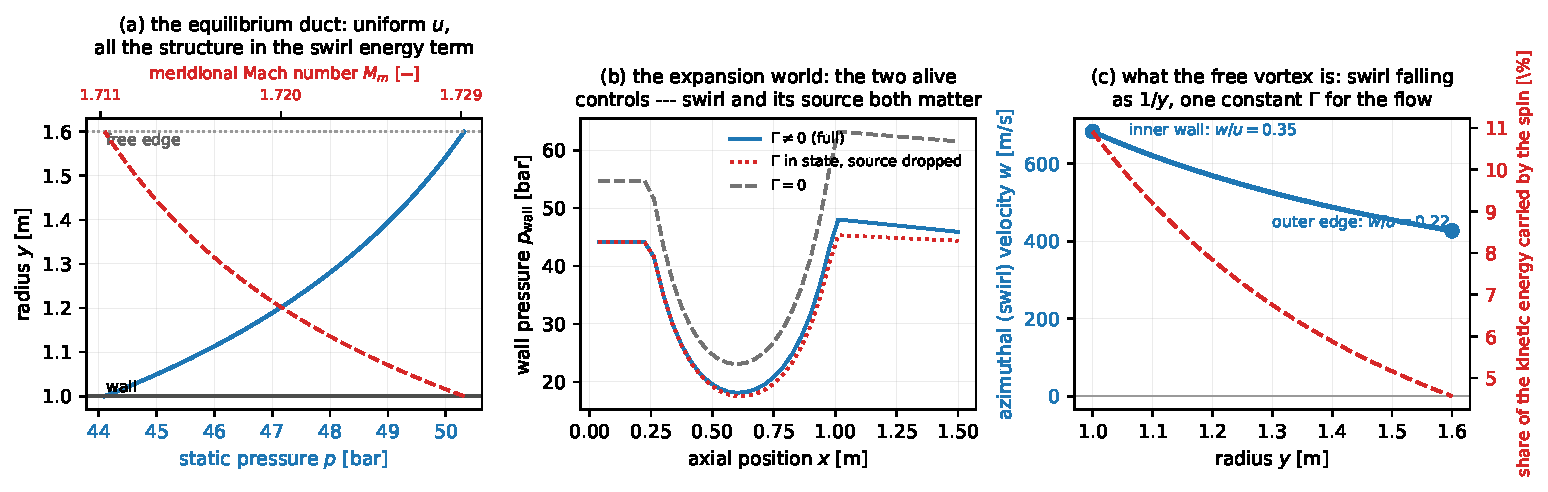
\includegraphics[width=\textwidth]{fig_swirl.pdf}
\caption{Swirl a vortice libero, misurato. (a)~Il condotto a
equilibrio radiale, una risposta nota esatta: raggio $y$ [m] in
verticale, pressione statica $p$ [bar] e numero di Mach meridiano $M$
[--] in orizzontale (due scale). La pressione sale e il numero di
Mach cala verso il raggio esterno benché la velocità assiale sia
uniforme e la velocità radiale sia nulla --- l'intera struttura
radiale è portata dal termine di swirl nel bilancio energetico. La
marcia conserva questo stato a $10^{-15}$. (b)~Il mondo in
espansione: coordinata assiale $x$ [m] contro pressione di parete
$p_w$ [bar], per tre esecuzioni --- swirl completo, swirl con la
sorgente centrifuga deliberatamente eliminata, e nessuno swirl. Le
tre curve si separano molto oltre le bande d'errore ammesse
($8.6\times$ e $12\times$), il che dimostra che sia lo swirl sia il
suo termine sorgente sono collegati e rilevanti. (c)~Che cosa il
vortice libero modella davvero: raggio $y$ [m] contro velocità
azimutale $w = \Gamma/y$ [m/s] --- la rotazione media nel tempo dello
scarico anulare, più veloce al raggio interno e in decadimento verso
l'esterno. È una \emph{media}, non il motivo di fase a spirale del
motore reale, che è fisica tridimensionale non stazionaria e
appartiene alla linea CFD (Sezione~\ref{sec:spiral}).}
\label{fig:swirl}
\end{figure}

\chapter{L'ingresso generale: una marcia per uno scarico non
uniforme}
\label{ch:generalinlet}

Il capitolo precedente si è chiuso su una frontiera: lo swirl a
vortice libero conserva esattamente la struttura caratteristica, e
qualunque cosa oltre esso rende il flusso \emph{rotazionale}, che la
marcia certificata non sapeva rappresentare. Questo capitolo rimuove
quella frontiera per il caso che conta per un RDE, e lo fa portando
qui una macchina che il codice arbitro possiede da sempre.

\section{Che cosa la marcia certificata assumeva, e perché contava}

Ogni nodo della marcia, finora, conservava quattro numeri: la
posizione e le due componenti di velocità, $(x, y, u, v)$. Nulla di
termodinamico veniva conservato, perché nulla serviva: lo stato del
gas era recuperato dalla \emph{sola velocità},
\begin{equation}
  h_t = h_0 - \tfrac12 q^2 \;\longrightarrow\; T
  \;\longrightarrow\;
  p = p_{\mathrm{ref}}\exp\!\Big(\frac{s(T) - s_0}{R}\Big),
  \label{eq:homentropic}
\end{equation}
con una singola entalpia di ristagno $h_0$ e una singola entropia
$s_0$ per l'intero campo. È l'ipotesi \emph{omoentropica}: un solo
serbatoio, una sola isentropica, ogni linea di corrente attinta dallo
stesso gas nello stesso stato.

Per un ugello alimentato da una camera di calma questo è esattamente
corretto. Per un motore a detonazione rotante è una scelta di
modello. L'anello reale consegna uno scarico che non è né uniforme né
privo di urti: la detonazione passa, i prodotti caldi seguono quelli
più freddi, e ogni linea di corrente arriva con la propria
temperatura totale e la propria entropia. La marcia non poteva
accettare dati simili --- non perché i numeri fossero difficili da
fornire, ma perché sarebbero stati \emph{sovradeterminati}. Dato un
profilo $(p, T, M)$ riga per riga, la marcia può onorare la velocità
e la direzione; la pressione che poi predice dalla
\eqref{eq:homentropic} è quella che dice l'isentropica globale, e se
la $p$ fornita non concorda non c'è dove mettere la differenza. Due
numeri su tre entrano; il terzo non ha casa.

\section{Che cosa l'arbitro faceva già}

Il codice Fortran indipendente ha varcato questa frontiera molto
tempo fa. Il suo modulo generico delle caratteristiche risolve il
classico processo elementare \emph{rotazionale}: entropia ed entalpia
di ristagno sono trasportate come \textbf{invarianti di linea di
corrente}, ogni cella localizza la linea di corrente che passa per il
suo nuovo punto, e lo stato al piede di quella linea è ricostruito da
\emph{invarianti interpolati} anziché da pressioni e densità
interpolate --- una distinzione che il registro di sviluppo di quel
codice annota come correzione, perché interpolare le grandezze
primitive fa uscire dalla varietà termodinamica mentre interpolare
gli invarianti non può farlo.

La conseguenza è esattamente la capacità che ci mancava: l'arbitro
legge da file un'intera linea iniziale punto per punto --- posizione,
densità, velocità, angolo, pressione, temperatura, Mach, $\gamma$ ---
e la marcia. Non c'era ragione di inventare una seconda risposta a un
problema già risolto. Questo capitolo porta qui la loro.

\section{Le tre modifiche}

\paragraph{I nodi portano la propria termodinamica.} Un nodo diventa
$(x, y, u, v, s, h_0)$: i due invarianti si uniscono ai quattro numeri
cinematici. La chiusura~\eqref{eq:homentropic} è invariata nella
forma e generalizzata nel contenuto --- ogni nodo usa i \emph{propri}
$(s, h_0)$ là dove la chiusura certificata usava la coppia globale.
Alla coppia globale le due coincidono identicamente, e il carrier
misura quell'identità anziché assumerla: la deviazione è esattamente
nulla, perché il percorso aritmetico è lo stesso.

\paragraph{Le equazioni di compatibilità cambiano forma.} Le celle
certificate risolvono la relazione di compatibilità gasdinamica
scritta in $(u, v)$. Quella forma è derivata assumendo flusso
irrotazionale, e per il teorema di Crocco i gradienti di entropia
\emph{sono} vorticità, quindi non sopravvive alla stratificazione. Il
processo elementare rotazionale usa invece la relazione lungo le
linee di Mach in pressione e angolo del flusso,
\begin{equation}
  \mathrm{d}\theta \pm Q\,\mathrm{d}p + S\,\mathrm{d}x = 0,
  \qquad
  Q = \frac{\sqrt{M^2-1}}{\rho q^2},
  \qquad
  S = \frac{\delta \sin\theta}{y\,M\,\cos(\theta \mp \alpha)},
  \label{eq:ptheta}
\end{equation}
che non richiede irrotazionalità: $Q$ è il coefficiente acustico
lungo una linea di Mach e $S$ è la sorgente assialsimmetrica che si
annulla nel flusso piano. Ogni coefficiente è valutato nello stato al
punto medio della propria corda, la forma implicita che le celle
certificate già usano.

\paragraph{La linea di corrente entra fra le incognite.} Una cella
interna risolve ora cinque numeri, $(x_4, y_4, u_4, v_4, t)$: la
posizione dai due incroci di linee di Mach, lo stato dalle due
relazioni~\eqref{eq:ptheta}, e $t$ --- il punto in cui la linea di
corrente che arriva al nuovo nodo attraversa la linea di dati a
monte. Gli invarianti nel nuovo nodo sono quelli della linea di dati
interpolati a quel $t$. Risolvere il piede \emph{insieme} al punto,
anziché iterare attorno a esso, è l'espressione naturale della stessa
fisica nell'ambiente a celle implicite di questo programma.

La parete e la frontiera libera non richiedono equazioni nuove:
entrambe sono linee di corrente, quindi ciascuna porta con sé, per
l'intera marcia, gli invarianti della riga da cui parte.

Con tutto ciò a posto, una linea $(p, T, M, \theta)$ riga per riga è
\textbf{esattamente determinata} --- tre numeri termodinamici per i
tre gradi di libertà dello stato $(s, h_0, q)$, più la direzione ---
e ripercorre la chiusura in andata e ritorno a quindici cifre.

\section{Due difetti colti dai test}

Entrambi sono registrati perché entrambi producevano uscite
plausibili.

\textbf{Il piede della linea di corrente usciva dalla propria corda.}
La prima versione interpolava gli invarianti lungo la corda che
congiunge i due punti di dati della cella. Su un getto stratificato la
marcia si rifiutava allora di convergere: raffinando la linea
iniziale l'errore restava dov'era, vicino a una parte su mille. La
sonda cella per cella ha mostrato perché. Ogni colonna scende di
circa $\tan\mu$ per la spaziatura delle stazioni, quindi appena le
righe sono abbastanza fini perché questo scorrimento superi la
spaziatura fra righe, la linea di corrente che arriva a un nodo cade
\emph{fuori} dalla corda fra i suoi due vicini --- e interpolare a
$t<0$ è estrapolare. Gli invarianti venivano allora trasportati lungo
una corda che non li conteneva. L'arbitro non ha questo difetto: la
sua cella cerca l'intersezione vera sull'intera colonna a monte.
Portata qui --- come \emph{decisione registrata}, nello stesso modo
in cui il piede di parete è sempre stato registrato --- l'errore di
trasporto nel corpo del getto è calato di due ordini di grandezza ed
è comparsa la convergenza (Figura~\ref{fig:s24rot}c).

\textbf{Un rigettatore va posto dove le equazioni portano carico.} La
verifica che corrompe un segno di compatibilità è stata dapprima
eseguita sul getto parallelo esatto, e \emph{ha promosso il codice
corrotto}: su quel mondo le differenze di pressione si annullano
identicamente, quindi il termine corrotto moltiplica zero e la marcia
corrotta riproduce la risposta giusta. Un rigettatore che non può
fallire non dimostra nulla. Spostato sul mondo del plug, dove le
stesse equazioni fanno lavoro reale, separa di tre ordini di
grandezza.

\section{Che cosa stabiliscono i test}

\begin{figure}[htbp]
\centering
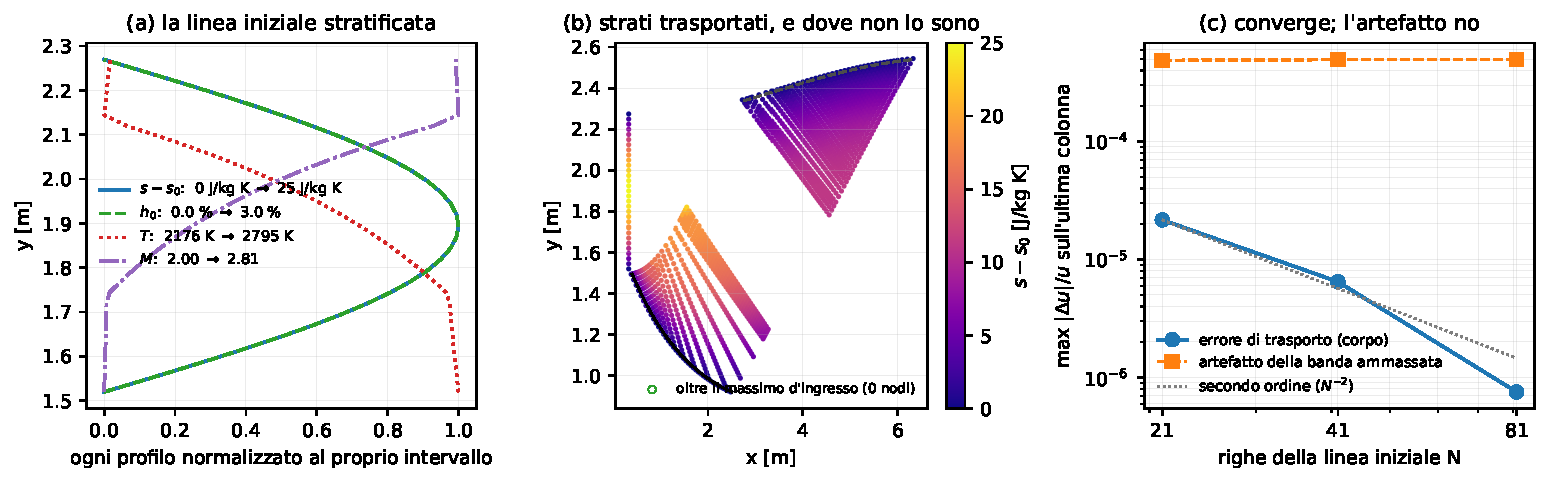
\includegraphics[width=\textwidth]{fig_s24_rotational.pdf}
\caption{L'ingresso generale, dall'esecuzione di riferimento. (a)~Una
linea iniziale stratificata: entropia, entalpia di ristagno,
temperatura e numero di Mach variano tutti attraverso il getto,
ciascuna curva normalizzata sul proprio intervallo con l'intervallo
stampato --- il tipo di dati che la marcia certificata non poteva
accettare. (b)~Il campo di entropia che la marcia trasporta
attraverso una spina: gli strati cavalcano le linee di corrente dalla
linea iniziale all'uscita, ed è questo l'aspetto che ha ``l'entropia è
un invariante di linea di corrente'' quando un solutore lo rispetta.
(c)~Verifica: l'errore di trasporto rispetto alla soluzione
stratificata esatta cala con il numero di righe della linea iniziale
all'ordine dello schema, mentre l'artefatto, riportato a parte, della
regola di crescita delle righe della maglia su un getto che non si
allarga non cala --- è topologia, non trasporto, ed è confinato a una
banda della colonna che la verifica esclude e dichiara.}
\label{fig:s24rot}
\end{figure}

La verifica usa una soluzione esatta per delimitare l'errore. Un
getto rettilineo a pressione uniforme, con temperatura e numero di
Mach diversi su ogni linea di corrente e senza angolo di flusso, è
una soluzione esatta delle equazioni assialsimmetriche: nulla ruota,
nulla si espande, e ciascuna linea di corrente si limita a portare a
valle il proprio stato. Se gli invarianti variano \emph{linearmente}
attraverso il getto anche l'interpolazione di cella è esatta, quindi
la marcia deve riprodurre la risposta all'arrotondamento --- misurato
$3\times10^{-8}$ su cinquecento celle certificate. Curvando la
stratificazione l'interpolazione diventa del secondo ordine, e
l'errore cala allora al raffinarsi delle righe:
$2.2\times10^{-5} \to 6.5\times10^{-6} \to 7.5\times10^{-7}$ su
$21 \to 41 \to 81$ righe, più rapidamente del secondo ordine che lo
schema promette.

Sul mondo del plug, a invarianti uniformi, le celle rotazionali e
quelle certificate sono due discretizzazioni delle stesse equazioni
continue, quindi non devono coincidere esattamente --- e
l'affermazione onesta è che la loro differenza \emph{si riduce}
all'ordine comune dei due schemi, da $3.0\times10^{-5}$ a
$8.8\times10^{-6}$ sotto raffinamento congiunto. Su una spina
genuinamente stratificata la marcia certifica a $0.058$, conserva la
massa a $8\times10^{-3}$ dopo la prima colonna, e trasporta il flusso
di entropia con una deriva di $5\times10^{-4}$ --- l'invariante
trasportato, misurato anziché assunto.

Un artefatto è riportato anziché assorbito. Su un getto che
\emph{non} si allarga, la regola di maglia che aggiunge una riga per
colonna --- scritta per uno scarico che si espande --- ammassa le
vecchie righe di bordo contro la frontiera stazionaria e apre un
vuoto in mezzo alla colonna. Le corde che attraversano quel vuoto
interpolano un profilo curvo lungo mezzo metro, e l'errore che ne
risulta non cala con il raffinamento perché è fissato dalla
topologia, non dalla spaziatura. È confinato alla banda ammassata, è
stabile all'uno percento sull'intera scala di raffinamento, e
l'affermazione sul trasporto è valutata al di sotto di esso. Le
geometrie di plug che questo programma progetta davvero sono scarichi
che si allargano e non lo sviluppano mai.

\section{Che cosa apre}

La conseguenza immediata è che uno scarico di RDE con vene calde e
fredde può essere marciato così com'è, anziché nella sua caricatura
uniforme in media; e poiché la linea iniziale che il port accetta
porta lo stesso contenuto del file dei valori iniziali dell'arbitro,
uno stesso ingresso può ora alimentare entrambi i codici --- il che
rende un confronto fra codici su un ingresso \emph{rotazionale} il
prossimo test naturale. Restano aperte e non misurate due ulteriori
questioni: se l'aggiunto del Capitolo~\ref{ch:spline} differenzi
attraverso una marcia stratificata così com'è (le celle passano per
la stessa macchina a solutore implicito, quindi dovrebbe), e se swirl
e stratificazione si compongano --- il vortice libero richiede
entalpia totale uniforme per il proprio argomento di
irrotazionalità, e uno scarico stratificato con swirl è
un'affermazione diversa, e più difficile.

\chapter{Confronto fra configurazioni, e l'angolo di ingresso}
\label{ch:compare}

Tutto fin qui ha certificato una macchina alla volta. Questo capitolo
pone la domanda che un progettista si fa davvero --- campana o plug,
quanto lungo, quanto swirl, a quale angolo di ingresso --- e scopre
che la parte difficile non è calcolare le risposte ma renderle
\emph{confrontabili}. Registra anche la più lunga svolta sbagliata di
questo programma: quattro sessioni spese a inseguire un difetto che
viveva in uno strumento di misura anziché nel flusso.

\section{La domanda, e perché è soprattutto una questione di
contabilità}

La spinta scala con la portata. Una campana calcolata in un mondo
posto in un certo modo, messa contro un plug calcolato in un altro,
confronta i \emph{mondi}, non i tipi di ugello. Perciò, prima che
qualunque confronto abbia senso, va fissata e imposta una base
comune:

\begin{itemize}[itemsep=1pt]
\item lo stesso gas, lo stesso stato di camera $(P_0, T_0)$, lo
  stesso ambiente $p_a$;
\item la stessa \textbf{portata} --- che porta un bonus, perché per
  una gola bloccata $\dot m = p_c A_t/c^{*}$, quindi portata uguale a
  stato di camera uguale significa \emph{area di gola} uguale, e
  perciò il coefficiente di spinta $C_F = F/(p_c A_t)$ e l'impulso
  specifico sono numeri direttamente confrontabili con la dimensione
  della macchina divisa via;
\item lo stesso \textbf{ingombro}: a ogni configurazione è concesso
  lo stesso raggio massimo. Un plug cui si conceda raggio illimitato
  vince banalmente sulla sola espansione.
\end{itemize}

Ogni configurazione è poi ottimizzata rispetto alla \emph{propria}
variabile di progetto: la campana rispetto al rapporto di espansione,
i plug rispetto al punto in cui la spina viene tagliata.

Una sottigliezza rende i due lati la stessa grandezza fisica. Per un
razzo alimentato da una camera chiusa la spinta assiale eguaglia il
flusso di quantità di moto in gauge ambiente attraverso \emph{una
qualunque} superficie che copra l'intero scarico e racchiuda
l'hardware. Per la campana quella superficie è il piano di uscita.
Per il plug lo stesso teorema si applica alla linea iniziale della
marcia: il flusso lì contiene già la spinta di tutto ciò che sta a
monte, perché la frontiera di getto libero fra il labbro e quel
taglio contribuisce esattamente zero nel gauge ($p = p_a$ su di
essa). Quindi
$F_{\rm plug}(l) = F_{\rm in}(x_0) + \int_{x_0}^{l}(p_w - p_a)\,
2\pi y\,(-\mathrm{d}y)$ è la spinta totale dalla camera fino al
troncamento --- lo stesso oggetto di quella della campana.

\section{Risultati di riferimento}

\begin{table}[htbp]
\centering
\small
\begin{tabular}{lrrrr}
\toprule
configurazione & $F$ [MN] & $C_F$ [--] & $I_{sp}$ [s] & $L$ [m] \\
\midrule
campana, al suo ottimo di rapporto & 116.474 & 1.4654 & 279.62 & 7.34 \\
plug, spina completa               & 116.148 & 1.4613 & 278.84 & 6.00 \\
plug, troncato                     & 116.148 & 1.4613 & 278.84 & 3.69 \\
plug, troncato $+$ swirl           & 111.839 & 1.4071 & 268.49 & 2.56 \\
\bottomrule
\end{tabular}
\caption{Quattro configurazioni a un punto di funzionamento sulla
base comune della Sezione~1: stesso gas, camera, ambiente, portata
(e quindi area di gola) e raggio di ingombro. Spinta in meganewton,
coefficiente di spinta e impulso specifico adimensionale e in
secondi, lunghezza in metri.}
\label{tab:configcompare}
\end{table}

\textbf{La campana vince dello $0.282\%$, e il risultato è
risolto.} La banda derivata sulla spinta viene dal raffinamento della
marcia stessa: $J = 1.161610, 1.161481, 1.161454 \times 10^{8}$~N a
tre risoluzioni, differenze successive $1.287\times10^{4}$ e poi
$2.737\times10^{3}$ --- un rapporto di $4.70$, che conferma il
secondo ordine --- da cui una banda di Richardson di
$1.09\times10^{4}$~N, ovvero lo $0.0094\%$. Il divario
campana--plug di $3.28\times10^{5}$~N vale $30\times$ quella banda.

\textbf{Il plug eguaglia la campana in metà lunghezza}, 3.69~m contro
7.34~m, che è il risultato dell'aerospike enunciato nel modo in cui
la termodinamica permette di enunciarlo
(Sezione~\ref{sec:ceiling}).

\textbf{Lo swirl costa il $4.0\%$}, un ordine di grandezza più di
qualunque differenza geometrica della tabella --- ma la spina con
swirl scende fino a $38\times$ sotto l'ambiente, un regime in cui un
flusso reale separerebbe e questa marcia non viscosa non può
seguirlo. Quel numero è indicativo, ed è etichettato come tale.

\begin{figure}[htbp]
\centering
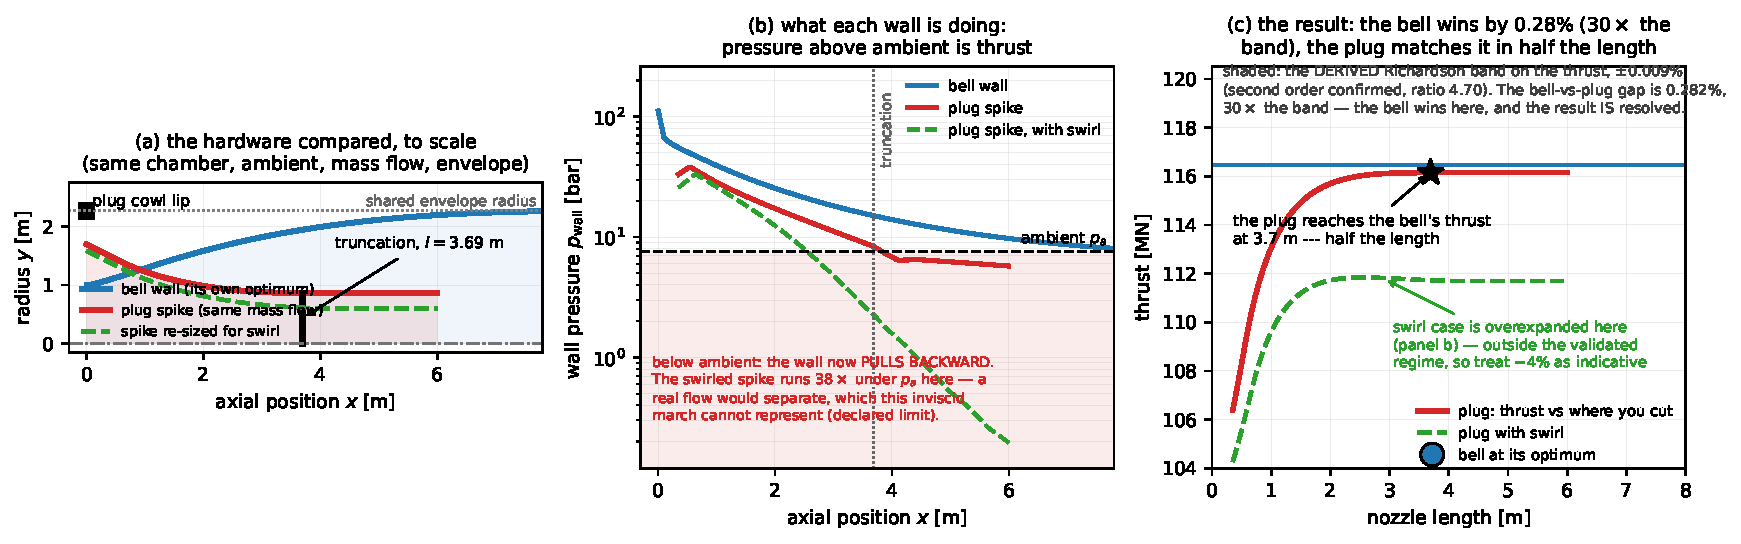
\includegraphics[width=\textwidth]{fig_config_compare.pdf}
\caption{Le configurazioni a confronto. (a)~L'hardware in un'unica
scala, posizione assiale e raggio in metri: la parete della campana
al proprio ottimo, la spina del plug adattata in massa, il suo
troncamento e la spina ridimensionata per lo swirl. (b)~Pressione di
parete in bar contro la linea dell'ambiente: sopra di essa la parete
fa spinta, nella regione ombreggiata sotto la parete tira
all'indietro --- e la spina con swirl entra molto dentro quella
regione. (c)~Spinta in meganewton contro lunghezza dell'ugello: la
curva del plug sale e satura, raggiungendo la spinta della campana
(blu) a circa metà della sua lunghezza. La banda ombreggiata è la
banda di Richardson \emph{derivata} sulla spinta, $\pm0.009\%$; il
divario campana--plug vale $30\times$ essa.}
\label{fig:configcompare}
\end{figure}

\section{Perché sono così vicine: il tetto termodinamico}
\label{sec:ceiling}

La quasi uguaglianza dei coefficienti non è una coincidenza né una
delusione. Entrambi gli ugelli espandono lo stesso gas dalla stessa
camera alla stessa pressione di uscita, e la sola conservazione
dell'energia fissa allora la velocità di uscita:
$\tfrac12 q_e^2 = h_0 - h(p_a)$ dà $q_e = 2742.136$~m/s senza alcuna
geometria nell'enunciato. Poiché la base impone la stessa portata, la
spinta ideale di quantità di moto
$\dot m\,q_e = 1.16474\times10^{8}$~N è esattamente la spinta
misurata della campana --- un'identità, perché al proprio ottimo la
campana è perfettamente espansa (il termine di pressione si annulla)
e la sua uscita è esattamente assiale (misurata a
$\theta_e = -10^{-16}$ nel Capitolo~\ref{ch:score}).

La campana sta \emph{sul} tetto. La geometria può quindi soltanto
perdere rispetto a essa, per divergenza, non uniformità ed espansione
incompleta --- tutti effetti dell'ordine dell'uno percento. È tutto
qui il campo da gioco dell'ottimizzazione di contorno, ed è il motivo
per cui questo programma deriva ogni tolleranza invece di
sceglierne una.

\section{Un vuoto di certificazione che il confronto ha esposto}

Predisporre il lato plug ha richiesto di porre il flusso come fa un
vero aerospike: arrivando al labbro puntato \emph{verso l'interno}
così che il ventaglio lo riporti verso l'assiale, con la spina
discendente verso l'asse. Ogni mondo di plug assialsimmetrico
certificato in questo documento pone l'opposto --- ingresso assiale,
il ventaglio che lo ruota \emph{verso l'esterno}, la ``spina'' che si
alza allontanandosi dall'asse (Figura~\ref{fig:turndir}a).

Non sono immagini speculari. Il termine sorgente assialsimmetrico è
$\delta\,c^2 v/y$ e $y$ è sempre positivo, quindi
$\theta \to -\theta$ non è una simmetria: il caso verso l'esterno
corre con $v > 0$ e $y$ crescente, quindi la sorgente si indebolisce
lungo la marcia, mentre il caso verso l'interno corre con $v < 0$ e
$y$ decrescente, quindi si rafforza. L'oracolo piano è immune
(nessuna sorgente, simmetria speculare genuina), quindi è
specificamente la certificazione \emph{assialsimmetrica} ad aver
esercitato sempre e solo un lato.

La rotazione verso l'esterno non è mai stata un progetto candidato
--- era un banco di prova. Un plug che ruota verso l'esterno lascia
l'intero scarico a $\theta_E > 0$ e raccoglie solo $\cos\theta_E$
della quantità di moto: $10.6\%$ perso alla rotazione di progetto di
$26.7^{\circ}$, contro nulla per un progetto verso l'interno. È il
modo naturale di scrivere un campo di prova a getto di spigolo in
forma chiusa, ed è così che è diventato l'unico caso testato.

\begin{figure}[htbp]
\centering
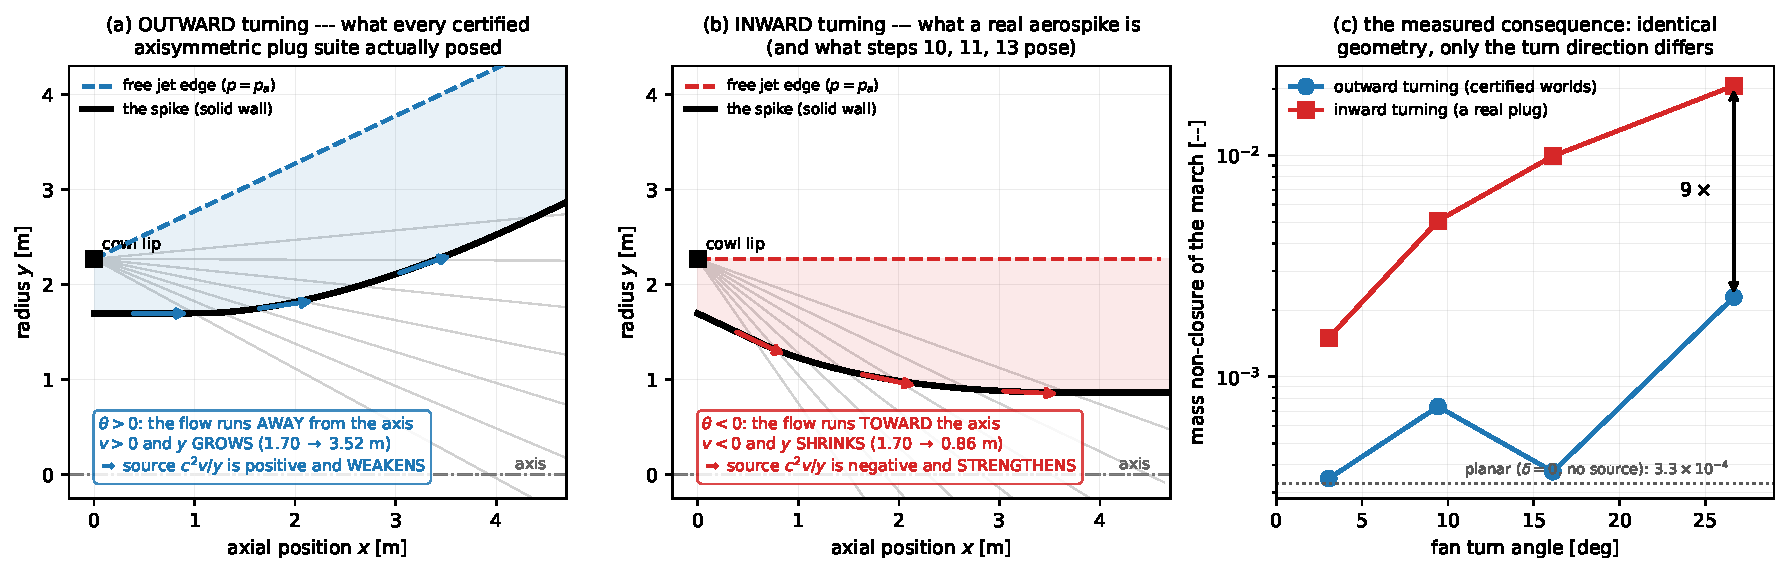
\includegraphics[width=\textwidth]{fig_turn_direction.pdf}
\caption{Rotazione verso l'esterno contro rotazione verso l'interno,
posizione assiale e raggio in metri. (a)~Ciò che ogni suite
assialsimmetrica certificata poneva: il flusso arriva assiale, il
ventaglio lo ruota verso l'esterno e la ``spina'' si alza
allontanandosi dall'asse; $v>0$, $y$ cresce, la sorgente si
indebolisce. (b)~Ciò che un vero aerospike è, e ciò che questo
capitolo pone: il flusso arriva puntato verso l'asse, il ventaglio lo
riporta indietro, la spina scende; $v<0$, $y$ decresce, la sorgente
si rafforza. (c)~La conseguenza misurata, in termini di non chiusura
di massa della marcia contro l'angolo di rotazione del ventaglio: la
rotazione verso l'esterno resta al pavimento senza sorgente
(punteggiato) e rimane piatta, quella verso l'interno sale a
$2\times10^{-2}$.}
\label{fig:turndir}
\end{figure}

\section{L'oracolo del flusso radiale}
\label{sec:radialoracle}

Per scoprire se quella differenza fosse un difetto, il programma
aveva bisogno di una soluzione assialsimmetrica esatta con il flusso
diretto \emph{verso} l'asse. Il flusso radiale sferico ne fornisce
una: ogni linea di corrente è un raggio uscente da un punto
sull'asse, la velocità dipende solo dalla distanza da esso, e la
continuità con l'isentropica la chiude come
$\rho(q)\,q\,r^2 = \mathrm{cost}$. Mettendo il punto singolare a
monte si ottiene un flusso divergente ($v>0$); mettendolo a valle uno
convergente ($v<0$). Un'unica formula, quindi i due casi non
differiscono in nulla se non nel segno che le equazioni vedono. E
poiché le linee di corrente sono raggi, un cono è una parete
\emph{esatta}.

\carrier{validation/a1\_source\_flow\_oracle.py}, \textbf{6/6 PASS.}
Il bordo libero è escluso per costruzione: entrano nel confronto solo
i punti sotto un limite rigoroso di dipendenza --- una retta dalla
sommità della linea iniziale con la pendenza caratteristica più
ripida presente nel campo, che nulla proveniente dall'alto può
superare. Rispetto alla forma chiusa, gli errori mediani sono

\begin{center}
\small
\begin{tabular}{lrr}
\toprule
 & convergente ($v<0$) & divergente ($v>0$) \\
\midrule
pressione di parete & $7.9\times10^{-4}$ & $5.2\times10^{-4}$ \\
interno $|\Delta q|/q$ & $3.4\times10^{-4}$ & $1.8\times10^{-4}$ \\
\bottomrule
\end{tabular}
\end{center}

\noindent Le celle interne e quelle a parete assegnata sono pulite
per flusso che ruota verso l'interno. Una trappola utile è emersa
costruendo il controllo negativo: nel flusso radiale \emph{ogni} cono
è una linea di corrente esatta, quindi perturbare l'angolo del cono
produce semplicemente un'altra soluzione esatta e non può mai
rigettare. Il rigettatore valido incurva la parete allontanandola dal
raggio, rompendo la proprietà di raggio, e separa di $29\times$.
Anche i rigettatori vanno scelti in base alla fisica --- la stessa
lezione dell'Appendice~\ref{app:f2rejector}, incontrata di nuovo.

\section{Lo strumento, non il flusso}

La non chiusura di massa che ha dato origine a questa indagine è in
larga parte una proprietà del misuratore. La verifica di
conservazione integrava sull'\emph{ultima colonna} della marcia, che è
una caratteristica, non un piano, e le cui lunghezze di segmento sono
selvaggiamente disuguali: su una spina discendente la più lunga è
$0.84$~m contro una media di $0.064$~m. L'errore trapezoidale scala
con il quadrato del segmento, quindi quell'unico segmento dominava.
Tre misure risolvono la questione: il flusso proprio della linea di
corrente del bordo libero è $4\times10^{-11}$ --- zero di macchina,
quindi non perde nulla; la parete perde lo $0.016\%$; e le celle
riproducono la soluzione esatta di cui sopra. L'ispezione colonna per
colonna trova la causa: solo la \emph{prima} colonna marciata ha un
buco di copertura, $26\times$ la spaziatura media fra righe quando la
parete sale e $39\times$ quando scende, contro $0.5$--$1.0\times$ per
ogni altra colonna --- perché una colonna è una caratteristica mentre
una linea iniziale verticale non lo è, quindi la prima colonna deve
da sola fare da ponte fra le due geometrie.

La lezione è quella che vale la pena portarsi dietro: \textbf{quando
la grandezza di interesse ha una banda derivata disponibile in modo
diretto, la si derivi in modo diretto.} L'incertezza sulla spinta era
stata dedotta da un misuratore di conservazione che misurava
qualcos'altro; raffinare la marcia e lasciarle misurare il proprio
errore --- la prima regola stessa del programma --- ha risolto la
questione in una sola esecuzione.

\section{L'angolo di ingresso come variabile di progetto}
\label{sec:inletangle}

Per direttiva del proprietario l'angolo di rotazione iniziale non è
più posto: fa parte dell'ottimizzazione. L'RDE consegna il proprio
flusso attraverso un ingresso anulare \emph{rettilineo} fra il raggio
iniziale della spina e il labbro del cowl, e l'inclinazione di quel
ingresso è la variabile di progetto.

La rotazione del ventaglio di labbro $\Delta\nu$ è fissata
dall'espansione (da $M_i$ fino a $p_a$) e non dipende dall'angolo di
ingresso, quindi l'angolo di scarico è semplicemente
$\theta_E = \theta_i + \Delta\nu$; la spazzata è riportata in
$\theta_E$ perché è quello che interessa alla fisica, e la classica
condizione di progetto è $\theta_E = 0$. La base della Sezione~1 è
invariata, con un'aggiunta: il flusso assiale di massa attraverso un
ingresso inclinato scala con $\cos\theta_i$, quindi l'anello viene
ridimensionato a ogni candidato per mantenere la portata di
riferimento, e la spinta è confrontata a \emph{lunghezza fissa} così
che la lunghezza non venga barattata in silenzio contro l'angolo.

\carrier{validation/a1\_inlet\_angle\_opt.py}. La spazzata alla cieca
atterra a $\theta_E = 0$ --- la previsione della divergenza,
recuperata anziché imposta --- e la penalità misurata segue il
modello $\cos\theta_E$ in segno e ordine su tutta la finestra
ammissibile:

\begin{center}
\small
\begin{tabular}{rrr}
\toprule
$\theta_E$ [gradi] & misurata & modello $\cos\theta_E$ \\
\midrule
$-6$ & $-0.365\%$ & $-0.548\%$ \\
$-4$ & $-0.153\%$ & $-0.244\%$ \\
$-2$ & $-0.031\%$ & $-0.061\%$ \\
$0$  & migliore   & --- \\
$+2$ & $-0.068\%$ & $-0.061\%$ \\
$+4$ & $-0.224\%$ & $-0.244\%$ \\
$+8$ & $-0.799\%$ & $-0.973\%$ \\
$+12$& $-1.753\%$ & $-2.185\%$ \\
\bottomrule
\end{tabular}
\end{center}

Due cose vanno lette. La penalità misurata è sistematicamente
\emph{minore} della pura divergenza, perché la distribuzione di
pressione di parete compensa in parte --- il baratto che il modello
in forma chiusa non contiene. E la curva è asimmetrica: ruotare verso
l'interno oltre l'ottimo costa meno che ruotare verso l'esterno dello
stesso angolo, che è la forma quantitativa della premessa della
direttiva secondo cui gli aerospike che ruotano verso l'esterno non
sono competitivi. La finestra è limitata dal lato interno dalla
geometria, non da una preferenza: a $\theta_E = -8^{\circ}$ la spina
scende a $y = 0.32$~m e la marcia perde la certificazione mentre il
flusso corre verso l'asse, dove la sorgente assialsimmetrica diverge.

\chapter{The free-form spike: a shape basis and a gradient}
\label{ch:spline}

Every plug computed so far in this document inherited its shape. The
spike was a \emph{streamline} of the expansion fan at the cowl lip:
you start at a radius and integrate the flow direction downstream, and
the contour is whatever comes out. Nothing was ever chosen. The only
two knobs were the angle at which the flow arrives
(Chapter~\ref{ch:compare}) and the station at which the spike is cut
(Chapter~\ref{ch:plugcycle}).

This chapter gives the spike a \emph{shape}: a family of contours with
free parameters, a derivative of thrust with respect to each of them,
and an optimizer that moves them. It is the last structural piece of
the program, and it is what finally makes the plug and the bell
comparable at equal freedom.

\section{Why the inherited contour is not the answer}
\label{sec:whynotstreamline}

The streamline construction is not arbitrary --- it solves a real
problem, exactly. Take the centred expansion fan that springs from the
cowl lip and let the spike follow a streamline through it: every
characteristic completes its turning, the flow leaves axially, and the
exit pressure lands exactly on ambient. That is the \emph{ideal},
full-length plug, and for that problem the streamline is optimal.

Then the spike is cut at a finite length. The contour was shaped to
deliver a downstream state that is now never reached, and nothing in
its construction knows the cut exists. The criterion that produced it
is no longer the criterion being maximized.

What the fixed-length problem rewards is visible in the thrust
integral itself. The axial force the spike collects is
\begin{equation}
  J_{\text{wall}} \;=\; \int (p - p_a)\, 2\pi y \,(-\mathrm{d}y),
  \label{eq:wallpush}
\end{equation}
and the weight is $2\pi y$: a given overpressure is worth far more
where the spike is still \emph{fat} than near its tip, simply because
there is more area there for it to act on. Under a length constraint
the right move is therefore to bias the expansion --- hold the
pressure up early, at large radius, and accept a worse state at the
end that is about to be discarded anyway. The streamline cannot do
this. It distributes its turning as though the whole contour mattered
equally, because it is not choosing: it is being traced.

This is Rao's argument for the bell (Chapter~\ref{ch:referee}),
transposed. His problem \emph{is} the length-constrained one, and the
multiplier $\lambda_3$ that Section~\ref{sec:o33} certified against
the automatic adjoint is precisely the shadow price of that length
constraint. The plug carries the same variational structure. What was
missing was not the theory but the machinery to act on it.

\section{The basis is borrowed, deliberately}

The wall is a \textbf{clamped-left natural cubic spline}: a curve
assembled from cubic pieces joined so that value, slope and curvature
are continuous across every join, pinned at its left end to a
prescribed height and slope. Its free parameters are the heights
$y_1, \dots, y_m$ at $m$ fixed stations, called \emph{knots}.

This is not a new basis written for the plug. It is the same routine
the bell optimizer uses, called directly. That choice is deliberate on
three counts. A bell-versus-plug comparison is only honest if both
sides have the \emph{same} shape freedom, which requires the same
basis. Any property already established for that basis --- in
particular that adding knots eventually represents any smooth contour
--- transfers without re-argument. And the adaptive-knot machinery
built for the bell, which decides \emph{where} knots should go rather
than accepting them evenly spaced, applies to this wall unchanged.
Section~\ref{sec:reprladder} shows that the plug needs it more than
the bell does.

\section{What is free, and what is not}

The design vector is
\begin{equation}
  W \;=\; [\,y_1,\; y_2,\; \dots,\; y_m\,],
\end{equation}
the spike radius at $m$ frozen stations spanning the contour, with the
last knot sitting exactly at the design length $L$.

Three quantities are \emph{not} free, and each for a reason.

\emph{The length} is fixed by placing the final knot at $L$. Without
it the optimization has a trivial answer: a longer spike always
collects more, so the optimizer would simply run away. Fixing the
length is what makes the problem well posed, and it is the same
constraint Rao imposed.

\emph{The mass flow} is fixed by construction. The starting radius of
the spike is found by a root search so that the flow crossing the
inlet station carries the reference mass flow. That station lies
\emph{upstream} of every knot, and the data on it are built from the
fan alone, so no shape parameter can reach it: the mass constraint and
the shape parameters are exactly independent. This is a structural
fact about the construction, not a numerical coincidence, and it means
the optimizer never has to trade thrust against mass.

\emph{The slope at the start} is fixed by physics. A wall is a
streamline, so where the incoming flow meets it the wall must run
along the flow. The clamped left slope is therefore the local flow
angle, not a design choice.

The inlet angle itself --- the inclination of the straight line by
which the engine delivers its flow --- remains the outer variable that
Chapter~\ref{ch:compare} swept, and it is not re-optimized here. The
two freedoms are kept apart so that a gain in thrust is attributable
to one of them rather than to their sum.

\section{The gradient: an adjoint through a frozen schedule}

The optimizer needs $\partial J/\partial y_k$ for every knot. Finite
differences would cost two marches per knot and would inherit the
step-size dilemma; the program has a better instrument.

The march makes \emph{decisions} as it goes --- which stations bracket
a wall point, how the cells are wired together. Those decisions are
discrete, and a derivative cannot be taken through them. The device,
used already by the bell optimizer, is to \textbf{record} them: one
march runs with concrete arithmetic and writes down every decision it
made, and every later evaluation \emph{replays} that record, treating
the decisions as frozen constants while the arithmetic stays
differentiable. The result is the exact derivative of the flow
\emph{at fixed topology}, obtained in one reverse pass regardless of
how many knots there are.

The record is refreshed whenever the optimizer accepts a step, so the
frozen topology is never allowed to drift far from the true one. The
agreement between this adjoint and central finite differences is
measured at every run and is reported in Section~\ref{sec:splineres}.

\section{The driver: trust-region SQP, in full}
\label{sec:splinedriver}

The optimizer deserves a complete description, both because every
number in this chapter and the next was produced by it and because
three of its defects --- each yielding plausible output while being
wrong --- are lessons in themselves.

\paragraph{What SQP is.} Sequential quadratic programming attacks a
nonlinear optimization by solving a sequence of tractable stand-ins:
at the current design $W$ it builds a \emph{quadratic model} of the
objective --- the measured gradient plus a curvature matrix
accumulated from successive gradient differences (BFGS: the model
learns curvature as it walks, no second derivatives are ever
computed) --- and, when constraints are present, a linear model of
those; the model problem is solved exactly, the true objective is
evaluated at the proposed step, and the cycle repeats. In the
\emph{trust-region} variant the model problem is solved only within
a radius $\Delta$ around $W$ --- the region where the model is
trusted --- and the ratio of \emph{actual} to \emph{predicted}
improvement governs $\Delta$: a step that delivers what the model
promised grows the radius, a step that does not shrinks it and is
rejected. This is the standard machinery for smooth nonconvex
problems, and the implementation underneath is scipy's
\code{trust-constr}.

\paragraph{Why the constrained problem arrives unconstrained.} The
three constraints of Section~15.3 --- mass, length, tangency ---
are imposed \emph{by construction} (the start radius by root
search, the last knot pinned at $L$, the clamped slope), so the SQP
never sees them: what remains is bound-free maximization over the
knot heights, and the sequential-quadratic machinery reduces to
trust-region quasi-Newton. The structure that makes the driver
nontrivial is not the constraints but the \emph{objective}: $J$ is
differentiable only through a frozen march record
(Section~15.4), and the record is itself position-dependent.

\paragraph{Decisions, records, and replays --- the vocabulary,
concretely.} Three words carry this section and deserve exact
meanings.

A \emph{decision} is any discrete choice the march makes while
building the field --- an integer or a branch, not a number that
varies smoothly with the design. The march makes thousands: which
segment of the previous column \emph{brackets} the characteristic
arriving at a new wall point (the wall-foot search returns an index,
and stepping columns further back changes that index by whole
units); how many rows a given column carries (the mesh gains a row
per column as the jet widens, and \emph{when} it gains one is a
threshold test); which cells are wired to which neighbours; which
side of every safety guard the arithmetic lands on. Each decision is
a step function of the knot heights: nudge the wall and the bracket
index, say, stays put --- until some threshold is crossed and it
jumps by one. A derivative cannot pass through a jump, so the march
as written is not differentiable, even though every formula inside
it is.

The \emph{record} (or \emph{schedule}) is the cure: one march runs
with concrete arithmetic and writes down every decision it made ---
the bracket indices, the row counts, the wiring, the branch
outcomes --- as plain integers in a ledger. Nothing about the flow
is stored; only the choices.

A \emph{replay} re-runs the march with every decision \emph{read
from the ledger instead of recomputed}. The comparisons and searches
vanish; what remains is a fixed pipeline of smooth
arithmetic --- the same cells, wired the same way, solving the same
equations --- through which the knot heights flow. That pipeline
\emph{is} differentiable, and one reverse pass through it yields
the exact gradient of $J$ \emph{at frozen topology}: the derivative
of the flow the march would compute \emph{if it kept making the
same choices}.

The price is locality, and it is the price the whole driver is
shaped around. Near the recorded base the frozen choices are the
right ones and the replayed $J$ agrees with the true $J$ to
round-off. Move the design far enough that the true march would
have decided differently --- a bracket shifts, a column gains its
row earlier --- and the replay, still faithfully executing the old
choices, computes a flow the true march would never produce: the
replayed objective is only \emph{piecewise} smooth, exact within
each decision cell and wrong across its boundary. The fold in
Figure~\ref{fig:s23driver}(b) is such a boundary seen edge-on, and
the finite-difference noise that once condemned a correct adjoint
(the ladder lesson of Section~15.6) is the same boundaries seen at
step-size scale.

\paragraph{The segmented walk.} Everything above dictates the
driver's shape: walk only on a record, distrust the walk the moment
it may have out-run the record's validity, and refresh the record
whenever a step is worth keeping. The driver therefore proceeds in
\emph{segments}:

\begin{enumerate}
\item \textbf{Record} at the current base $W$: one concrete march,
  writing down every discrete decision. The record must be
  \emph{Newton-certified} (every cell converged to round-off); an
  uncertified record rejects the base outright.
\item \textbf{Walk on the record}: one \code{trust-constr} call,
  limited to a few model iterations, maximizes the \emph{replayed}
  $J$ --- exact value and exact adjoint gradient at frozen topology
  --- inside the driver's own radius.
\item \textbf{Treat the endpoint as a trial, not an answer.} The
  fresh record at the endpoint must certify, and the replayed $J$
  there must beat the incumbent. Acceptance re-records and grows
  the radius ($\times 1.5$, capped); rejection reverts to the best
  certified design and halves the radius toward a floor.
\item \textbf{Stop} when a trial is worse at the radius floor, when
  the walk stops moving at the floor, or at the segment budget. The
  answer is the \emph{best certified design ever seen}, never the
  last endpoint.
\end{enumerate}

Figure~\ref{fig:s23driver}(a) shows a production walk in this
discipline --- fifteen accepted bases, three trials rejected for
thrust, two bases rejected by the certification gate, five
no-motion retries --- worth a thousand words of pseudocode.

\begin{figure}[htbp]
\centering
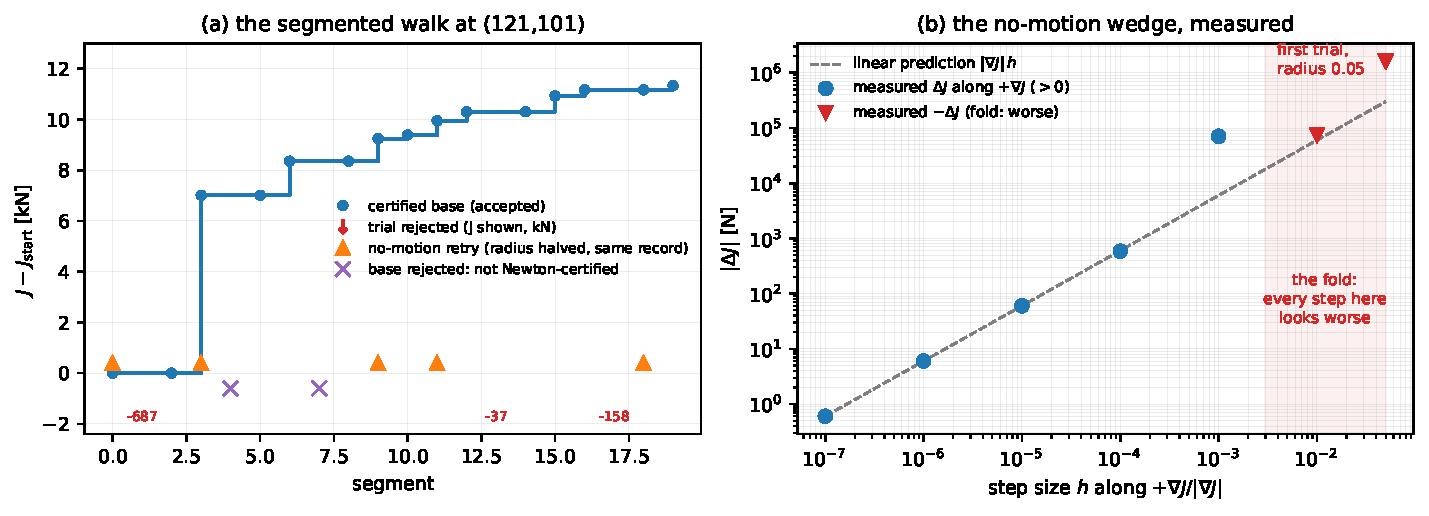
\includegraphics[width=\textwidth]{fig_s23_driver.pdf}
\caption{The driver at work, from the run of record. (a)~The
segmented trust-region SQP re-optimizing the spike at the doubled
resolution: the staircase is the accepted thrust (relative to the
start, in kN); red arrows mark trials the acceptance test rejected
(their thrust printed below, in kN --- the worst overshoot is
$-687$ kN, which the old driver would have adopted); purple crosses
mark bases rejected by the per-cell Newton certification gate;
orange triangles mark no-motion retries, where the inner solver
returned its start point and the outer driver halved the radius and
tried again on the same record. (b)~The mechanism behind those
retries, measured: thrust along the gradient direction is smooth and
matches the linear prediction (dashed) over five decades of step
size, then \emph{folds} near $h \sim 3\times10^{-3}$; a first
trial at the full radius $0.05$ lands deep in the fold, and the
inner solver's quadratic model, poisoned by that single rejected
step's spurious curvature, stops evaluating the objective and
returns the start point unchanged --- while $+7\times10^{4}$ N was
available at $h = 10^{-3}$.}
\label{fig:s23driver}
\end{figure}

Three defects surfaced across the campaigns, and all three are worth
recording because all three produced plausible output while being
wrong.

\textbf{No acceptance test.} The first version adopted the endpoint of
every segment unconditionally. A segment walks a local model on a
frozen record, so a long segment can walk clean past the region where
that model is valid and return a design that is genuinely worse. The
first run did exactly that: segment~1 improved the thrust, segment~2
overshot, and the carrier reported the overshoot as the answer --- a
\emph{loss} of $0.21\%$ presented as the outcome of a maximization. A
segment endpoint is a \emph{trial} point, and the fix is the standard
one: if the trial does not beat the incumbent, revert to the best
certified design and shrink the radius.

\textbf{A radius that undid its own shrinks.} With the acceptance test
in place the walk stopped losing, but it also stopped improving: it
oscillated between one good design and a succession of overshoots. The
cause was that the outer loop read its trust radius back from the
inner optimizer after each segment. That inner radius tracks the inner
method's own model, and adopting it silently overwrote every shrink
the outer loop had just ordered. Once the outer radius was kept as the
outer loop's own property --- grown only on an accepted design,
shrunk only on a rejected one --- the walk resumed and the gradient
fell by a further order of magnitude.

\textbf{The no-motion wedge.} The third defect waited for the
sharper instrument of Section~\ref{sec:gainresolved}. Started from a
converged coarse optimum at doubled resolution, the inner solver
returned its start point unchanged --- ``no motion'' --- with a
gradient of $6\times10^{6}$ in hand, and the driver, reading no
motion as convergence, stopped. The probe in
Figure~\ref{fig:s23driver}(b) exonerated the objective: smooth,
matching its linear prediction over five decades of step size,
folding over only beyond $h \sim 3\times10^{-3}$. The wedge is the
inner solver's: its first trial at the full radius lands past the
fold, the rejected step teaches its curvature model a violently
wrong lesson, and the poisoned model proposes nothing further worth
evaluating --- while $+7\times10^{4}$ N of improvement stood one
$10^{-3}$-step away. The repair stays inside the driver's own
semantics: no motion above the radius floor is treated exactly like
a rejected base --- halve the radius, retry on the same record ---
and only no motion \emph{at} the floor is convergence. Every
previously recorded walk reproduces bit-for-bit under the repaired
driver; the retries can be seen doing their work in
Figure~\ref{fig:s23driver}(a).

None of the three defects announced itself. The first produced a
confident wrong sign; the second a plausible-looking plateau easy to
report as convergence; the third a false ``converged'' verdict with
an order of magnitude of gradient still standing. One theme: the
optimizer's bookkeeping is part of the experiment, and it is graded
by the same standard as the physics.

A further gate is inherited rather than new: a design whose march
cannot be Newton-certified is rejected outright and the radius
shrunk. This fires in practice --- one segment of the S21 run of
record hit a record with a worst residual of $2.3$ and was reverted;
the purple crosses of Figure~\ref{fig:s23driver}(a) are the same
gate firing at the doubled resolution --- so it is load-bearing
rather than decorative.

\section{Does the basis contain the incumbent?}
\label{sec:reprladder}

Before any gain can be believed, one thing must be checked: can the
spline family even \emph{express} the contour it is starting from? If
not, an apparent improvement might only be the optimizer climbing back
out of a hole its own basis dug.

A spline on finitely many knots cannot reproduce the streamline
exactly, so the honest question is not whether the error is zero but
whether it \emph{falls} as knots are added. Measured on a ladder of
$6, 12, 24, 48$ knots, the largest deviation between the spline and
the streamline behaves as follows:

\begin{center}
\begin{tabular}{rccl}
\toprule
knots & max deviation & \% of spike drop & where it sits \\
\midrule
 6 & $6.536\times10^{-4}$ m & 0.0843\,\% & $x = 2.343$ m \\
12 & $4.451\times10^{-4}$ m & 0.0574\,\% & $x = 0.612$ m \\
24 & $3.418\times10^{-5}$ m & 0.0044\,\% & $x = 2.448$ m \\
48 & $2.309\times10^{-5}$ m & 0.0030\,\% & $x = 0.560$ m \\
\bottomrule
\end{tabular}
\end{center}

The total reduction across the ladder is a factor of $28$, so the
basis is dense in the sense required. But the ladder is not clean, and
its untidiness is the interesting part. From $6$ to $12$ knots the
error falls by only $1.5\times$, which for cubic interpolation of a
smooth curve is far too slow --- and taking that single ratio as the
verdict, as a first version of this check did, produces a failure
report about a basis that is in fact perfectly adequate.

Two different errors are competing, and the last column shows which
one is winning. One lives at the \emph{right} end, where the spline's
free end condition is imposed; the other sits at $x \approx 0.56$ to
$0.61$ m, the station where the streamline's curvature climbs from
essentially zero at the clamped start to its peak --- the one stretch
of the contour that genuinely bends. Neither dominates uniformly:
the location of the maximum alternates between them as knots are
added, which is exactly why no two adjacent counts can be trusted to
report a rate.

The lesson is a design lesson. Evenly spaced knots spend their budget
uniformly along a contour that is nearly straight over most of its
length, and starve the single region that curves. That is precisely
the situation the adaptive-knot machinery answers, and since this wall
uses the bell's basis, that machinery can be pointed at it without
modification. It is the natural next step and is listed as such in
Chapter~\ref{ch:status}.

One control matters here: the streamline being compared against is
itself a numerical integration, so it could in principle be the
inaccurate party. Refining its step size moves its endpoint by
$5.4\times10^{-8}$ m, nearly three orders of magnitude below the
smallest deviation on the ladder. The reference is not the
limitation.

\section{What the optimizer finds}
\label{sec:splineres}

The run of record uses six free knots on a spike of length $2.5$ m, at
the inlet angle Chapter~\ref{ch:compare} selected, in the same posed
world as every other configuration comparison.

The mass constraint is met to $4.8\times10^{-12}$ relative --- machine
precision, once the constraint is set and graded by the same
functional (Appendix~\ref{app:twoinstruments}) --- inside a derived
band of $3.8\times10^{-4}$.

The adjoint is verified next, and doing so honestly required
abandoning the obvious instrument. A finite difference cannot simply
be trusted here: the replayed march is only \emph{piecewise} smooth
in the design vector, because the wall-search topology is frozen at
the record and a perturbed design can sit fractionally on the wrong
side of a decision that record already made. Shrinking the step does
not fix this. Measured over steps of $10^{-4}$ down to $10^{-8}$, the
difference between the finite difference and the adjoint does not
fall as $h^2$; it \emph{wanders} --- for one node it runs
$-197, +61, +1.8, +0.63, -0.42$, and for another it never settles
below a fixed level at all. That is noise, not truncation, and a band
estimated from two steps describes none of it. An earlier version of
this check did exactly that and reported a correct adjoint as a
failure.

The reliable reading is the scatter itself. Taking central
differences on a ladder of steps small enough that truncation is
negligible, the spread across the ladder measures the difference's
own reliability, and that is what the adjoint may be graded against:

\begin{center}
\begin{tabular}{lccc}
\toprule
node & adjoint & difference & $|$discrepancy$|$ (band) \\
\midrule
0 & $+5.569035\times10^{6}$ & $+5.568800\times10^{6}$ &
  $2.4\times10^{2}$ $(5.2\times10^{2})$ \\
3 & $-3.523614\times10^{5}$ & $-3.523618\times10^{5}$ &
  $4.6\times10^{-1}$ $(6.3\times10^{1})$ \\
5 & $-1.119305\times10^{6}$ & $-1.119305\times10^{6}$ &
  $7.5\times10^{-4}$ $(2.1\times10^{1})$ \\
\bottomrule
\end{tabular}
\end{center}

\noindent and the directional identity $\langle \nabla J, v\rangle$
reads $9.63322\times10^{5}$ against $9.63302\times10^{5}$, a
discrepancy of $2.1\times10^{1}$ inside a band of
$1.6\times10^{2}$. Two of the three nodes agree with the adjoint far
below any plausible noise floor; the third is the one whose
difference was measured to be unreliable.

The walk then proceeds through seven accepted segments and nine
records:

\begin{center}
\begin{tabular}{lcc}
\toprule
 & $J$ [N] & $|\nabla J|$ \\
\midrule
streamline (start) & $1.15378731\times10^{8}$ & $5.844\times10^{6}$ \\
segment 1          & $1.15430463\times10^{8}$ & $1.837\times10^{6}$ \\
segment 4          & $1.15471843\times10^{8}$ & $1.681\times10^{6}$ \\
segment 5          & $1.15482085\times10^{8}$ & $2.306\times10^{5}$ \\
final              & $1.15483517\times10^{8}$ & $1.472\times10^{5}$ \\
\bottomrule
\end{tabular}
\end{center}

The gradient falls by a factor of $40$ and the thrust rises by
\begin{equation}
  \frac{J_{\text{spline}}}{J_{\text{streamline}}} - 1
  \;=\; +0.0908\,\%.
\end{equation}
In coefficient terms $C_F$ moves from $1.45163$ to $1.45295$. The
final spike descends monotonically from $1.4936$ m to $0.8330$ m and
clears the axis, so it remains a physically admissible inward-turning
contour.

\section{The gain is not resolved, and how that was found out}
\label{sec:notresolved}

The paragraph above states a gain. It does not state that the gain is
\emph{real}, and on the evidence of this carrier it is not yet
established.

An earlier version of this chapter compared the $+0.0908\%$ against a
thrust band of $0.0094\%$ and concluded it was ``about ten times the
band''. That band was inherited: it was derived in
Chapter~\ref{ch:compare} at a different resolution, on a different
computation. Quoting it here is the same error this program has now
met three times --- grading a result with an instrument that did not
produce it --- and it was flagged as a caveat before it was tested.

Testing it is cheap and the carrier now does it as check C-6: refine
the march that produced \emph{both} thrusts and let it measure its own
discretization error on the \emph{same} two designs, so whatever
cancellation the difference enjoys is preserved. On a run with ten
knots and twenty-six accepted segments:

\begin{center}
\begin{tabular}{lc}
\toprule
 & gain over the streamline \\
\midrule
at the carrier's resolution $(K, N)$      & $+0.1302\,\%$ \\
refined to $(2K-1,\; 2N-1)$               & $+0.0820\,\%$ \\
\midrule
band this refinement supports             & $0.1930\,\%$ \\
\bottomrule
\end{tabular}
\end{center}

\noindent The band is \emph{larger than the gain}. C-6 therefore
FAILS, and the honest reading is:

\begin{quote}
\textbf{It is not established that the free-form spike beats the fan
streamline. The measured gain lies inside the discretization error of
the computation that measured it.}
\end{quote}

This does not overturn the machinery, which is verified independently:
the adjoint against its finite differences, the basis against its
refinement ladder, the mass constraint to $5\times10^{-12}$, the
driver against its own rejector. Nor does it say the gain is absent
--- both evaluations are positive, and the refined one is still
$+0.082\%$. It says the experiment is not yet sharp enough to
distinguish a real gain of this size from its own noise, which is a
statement about resolution rather than about nozzles.

Two routes would sharpen it, and both are ordinary work: run at a
resolution where the band falls below the effect, and place the knots
where the contour bends (Section~\ref{sec:reprladder}) so that fewer
of them buy more shape. What should \emph{not} be done is to quote the
gain against a band borrowed from elsewhere, which is how the claim
came to look ten times stronger than it is.

\section{How much of this to believe}

The gain is small, and it should be. The exit speed of the exhaust is
fixed by energy alone, so a perfectly expanded design already sits
close to a ceiling that geometry cannot raise
(Chapter~\ref{ch:compare}). Against a near-optimal incumbent, a
recovery of one part in a thousand is the right order of magnitude; a
gain of several percent would have been evidence of a defect, not of a
better nozzle.

The measurement is also a \emph{differential} one, which is its main
protection: both thrust values come from the same march at the same
resolution, so discretization error largely cancels between them. The
band it is quoted against, however, was derived at the production
resolution of Chapter~\ref{ch:compare} and should be re-derived at
this carrier's resolution before the ratio is treated as final.

Three limitations are stated plainly. The final gradient is
$1.47\times10^{5}$, not zero, so this is a design the optimizer was
still improving when the segment budget ran out. Six knots is a small
basis, and Section~\ref{sec:reprladder} gives reason to expect that
adaptive placement would do better than more of them. And the result
stands at a single design point: one length, one inlet angle, one
ambient pressure. Above all,
Section~\ref{sec:notresolved} shows the gain is not resolved by this
carrier's own refinement, so it is a measurement awaiting a sharper
experiment rather than a result.

\section{The sharper experiment: knots bought where the contour bends}
\label{sec:adaptive}

Both routes proposed at the end of Section~\ref{sec:notresolved} have
now been run: knots placed by an error indicator rather than
uniformly, and the gain re-graded on a three-point resolution ladder
of the march that produced it. This section reports both, and the
second one is the result.

\paragraph{The indicator.} The adaptive procedure is the bell's
--- solve, mark the knot intervals that carry the residual, insert,
re-optimize, repeat --- with one substitution that the plug makes
possible. The bell reads its optimality residual off the flow, as the
drift of an adjoint-equal quantity along a control surface, because
that is the only access it has. The plug carrier owns its discrete
adjoint outright, so the same object is available directly: enrich
the basis with a candidate node at the midpoint of every knot
interval, re-interpolate the incumbent wall (for a cubic spline on a
knot superset with the same end conditions this reproduces the wall
\emph{exactly}, by uniqueness --- measured at $4\times10^{-16}$ m),
and read the gradient of thrust at the candidate nodes from one march
and one reverse-mode pass. At a class optimum the gradient at the
\emph{existing} nodes is negligible, so a candidate's component
measures precisely the freedom the current class cannot express.
The interval whose candidate carries $84.8\%$ of the total indicator
mass is the first one, $x \in [0.350, 0.565)$ --- the same
neighbourhood the representation ladder of
Section~\ref{sec:reprladder} identified from geometry alone.

\paragraph{One knot pays; a matched uniform knot does not.} Inserting
the marked candidate at $x = 0.4575$ m and re-optimizing from the
(exact) warm start raises the thrust by $+0.1921\%$ at the working
resolution. The control experiment gives that number its meaning: the
\emph{uniform} class at the same node count, optimized by the same
driver from the same kind of start, gains $+0.0002\%$ --- the extra
uniform knot lands where the contour is nearly straight and buys
nothing. Placement, not node count, is what pays. A second adaptive
insertion (at $x = 0.4037$) buys nothing further: the driver cannot
extract even one part in $10^{15}$, and the procedure stops itself
honestly. Whatever this basis can reach at this length, one
well-placed knot reaches it. Figure~\ref{fig:spikedesigns}
draws the designs as objects: the bulge the knot bought, the tail
both optimizers surrender, and the two classical machines the next
section compares against.

\paragraph{The ladder, and the verdict.} The gain of the adaptive
optimum over the fan streamline was then graded the way
Section~\ref{sec:notresolved} demands: both designs frozen, the march
refined twice, each rung re-posing its own start line, the band
derived from the ladder itself.

\begin{center}
\begin{tabular}{lcc}
\toprule
march resolution & adaptive ($m=11$) & uniform control ($m=11$) \\
\midrule
$(K, N) = (61, 51)$    & $+0.313\,\%$ & $+0.127\,\%$ \\
$(121, 101)$           & $+0.186\,\%$ & $+0.068\,\%$ \\
$(241, 201)$           & $+0.080\,\%$ & $+0.029\,\%$ \\
\midrule
band the ladder supports & $0.426\,\%$ & $0.157\,\%$ \\
\bottomrule
\end{tabular}
\end{center}

\noindent The band is still larger than the gain, at sixteen times
the cost of the original experiment. The claim that the free-form
spike beats the fan streamline remains \emph{not established} --- and
the ladder now says something sharper than ``not yet''. The measured
gain \emph{falls monotonically} under refinement, for the adaptive
design and for the uniform control alike, with a rung-to-rung decay
ratio near $0.84$. The reading: a large share of any coarse-grid gain
is the optimizer fitting the march's own discretization error ---
the design was tuned at the coarse resolution, so it is flattered by
exactly the error it was tuned against --- and the march converges
too slowly on this differential quantity for brute-force refinement
to win; each halving of the grid spacing removes only a sixth of the
remaining artifact while multiplying the cost by six.

\begin{figure}[htbp]
\centering
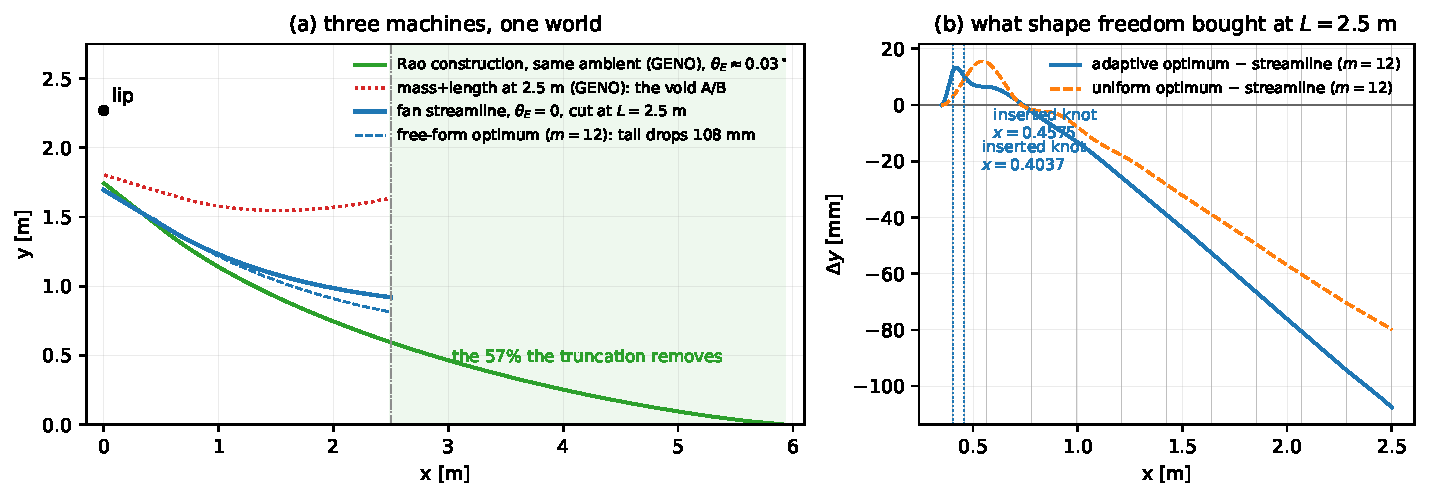
\includegraphics[width=\textwidth]{fig_spike_designs.pdf}
\caption{The designs this chapter compares, drawn as objects.
(a)~Three machines in one world, $x$ axial against $y$ radial [m]:
the fan-streamline spike with $\theta_E = 0$, cut at $L = 2.5$ m
(solid), with the free-form optimum of this section dashed --- the
two coincide over most of the length and separate at the tail, which
the optimizer pulls $87$ mm lower; the classical Rao construction
expanded to the same ambient (GENO, posed by exit Mach), whose spike
runs to the axis near $x = 5.9$ m --- the shaded region is the $57\%$
of it our fixed length removes; and the mass-plus-length design at
$2.5$ m, the machine of the void A/B of
Section~\ref{sec:vsrao}: with both of Rao's degrees of freedom
consumed, ambient becomes an output and its wall barely tapers.
(b)~What shape freedom actually bought at $L=2.5$ m: the adaptive
and uniform optima minus the streamline, in millimetres. \emph{Drawn
from the re-adjudication run of 2026-09-15
(Section~\ref{sec:readjudication}), not from the 08-10 record the
text of Section~\ref{sec:adaptive} describes:} the adaptive design is
now $m = 12$ with two inserted knots ($x = 0.4575$, then $0.4037$,
where the indicator put $90\%$ and $79\%$ of its mass), a $+13$ mm
bulge at $x = 0.42$ and a monotone dive to $-108$ mm at the exit; the
uniform $m = 12$ control bulges $+16$ mm at $x = 0.55$ and dives to
$-80$ mm. Both optimizers tell the same story (raise the wall where
pressure is high and large-radius, surrender radius at the tail) ---
and both, as Section~\ref{sec:readjudication} shows, do it with a
compression corner at the foot that folds the march. Thin vertical
lines mark the adaptive knot set.}
\label{fig:spikedesigns}
\end{figure}

\paragraph{What follows.} More knots are ruled out (the second
insertion bought nothing), and a longer ladder is a losing race (the
decay ratio says so). What remains is a better \emph{instrument}: an
incumbent optimized at the finer resolution, so that it is not tuned
to the coarse march's error; or an extrapolation of the paired
difference down the existing ladder, whose own band would settle
whether anything survives at the limit; or the exact two-route thrust
functional of Chapter~\ref{ch:status}, once its field residual is
understood. Until one of those runs, the honest summary of the
free-form spike is unchanged in verdict and sharpened in diagnosis:
the machinery is verified, the placement principle is demonstrated,
and the headline gain is a property of the instrument's resolution,
not yet of the nozzle.

\section{The gain, resolved}
\label{sec:gainresolved}

The better instrument has now been built and run, and the question
this chapter carried through three campaigns is closed. Three things
were done, in the order the evidence demanded.

\paragraph{Extrapolation, done per design.} Each design's thrust,
measured on a resolution ladder whose spacing halves per rung, is its
own convergent sequence, and each sequence must be extrapolated by
its own contraction --- the streamline's converges cleanly at first
order (measured ratio $0.506$), while a design tuned at a coarse
resolution is \emph{non-monotone} near its tuning rung and refuses a
one-mode fit. Extrapolated correctly, the S22 optimum's limit lands
$0.012\%$ \emph{below} the streamline's: the coarse-grid gain was not
merely unresolved, it was wholly the optimizer fitting the march's
discretization error, slightly past the point of self-harm.

\paragraph{An incumbent that is not tuned to the coarse march.} The
optimum was re-optimized at the doubled resolution $(121,101)$ ---
same class, same driver, sharper instrument. (Doing so exposed a
driver defect worth recording: from this start the trust-region
inner solver's first rejected trial, landing past the fold scale of
the replayed surface, poisoned its quadratic model and it returned
the start point unchanged while $+7\times10^{4}$ N of improvement
was measurably available at a step of $10^{-3}$. The outer driver
now applies its reject-and-shrink semantics to that case; every
previously recorded walk reproduces bit-for-bit.) The fine-tuned
optimum gains $+0.0098\%$ over the S22 design at its own resolution
--- and its ladder then repeats the pattern one rung later: whatever
resolution tunes the design, the march flatters it there and
retracts the flattery one rung above.

\paragraph{The paired ladder to $(1921,1601)$, and the verdict.}
The difference of the two designs, however, becomes a clean sequence
once the design leaves its tuning window, and it was extended to six
rungs --- affordable because a profiling pass found the march
spending its high-resolution hours inside a single degenerate
tensor-stacking compilation, which a one-line change (bit-identical,
gated on the record) reduced from hours to minutes:

Figure~\ref{fig:s23ladder} carries the result. Panel~(a) is the
whole story in one frame: the streamline's thrust climbs
monotonically onto its extrapolated limit with ratios locked at the
march's first order, while the optimum --- tuned at the second rung
--- overshoots there and then descends onto the \emph{same} limit;
the two designs are one nozzle measured two ways. Panel~(b) shows
the paired gain minus its extrapolated limit falling as a straight
line on a log scale --- geometric convergence, ratios printed at
each rung --- and the open marker is the sixth rung as the model
\emph{predicted it before it ran}: the miss is eighteen times
smaller than the step it predicted, which is the model earning its
extrapolation. That limit is

\begin{figure}[htbp]
\centering
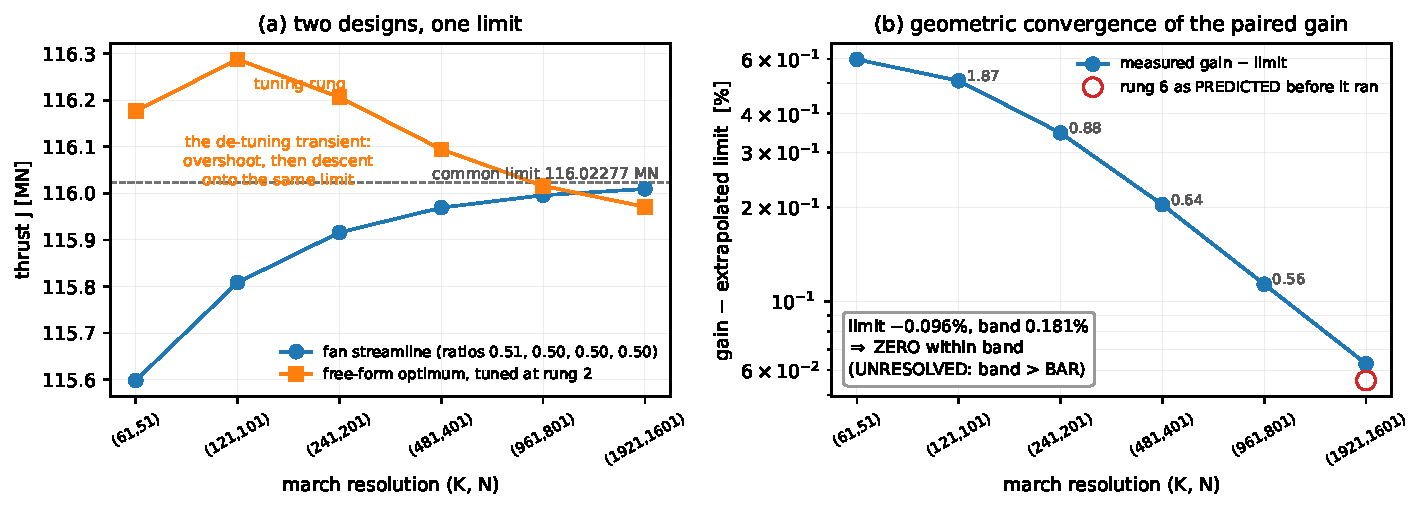
\includegraphics[width=\textwidth]{fig_s23_ladder.pdf}
\caption{The six-rung paired ladder, \emph{drawn from the
re-adjudication run of 2026-09-16} (Section~\ref{sec:readjudication};
the 08-11 record described in the text of this section is history and
its figure was lost). (a)~Thrust of both designs against march
resolution, spacing halving per rung: the fan streamline (blue)
converges monotonically at first order (successive-difference ratios
$0.51, 0.50, 0.50, 0.50$) onto the dashed extrapolated limit; the
re-adjudicated fine optimum (orange), tuned at the second rung from a
streamline start, is flattered there by the instrument's own
discretization error and descends past the streamline's limit as the
march sharpens. (b)~The paired gain minus its extrapolated limit: a
straight line on the log scale is geometric convergence, with the
ratio settling toward the march order (printed: $1.87, 0.88, 0.64,
0.56$); the open red circle is rung six as predicted from rungs three
through five before it was computed. The extrapolated limit,
$-0.096\% \pm 0.181\%$, is zero within its band but the band exceeds
the bar ($0.040\%$): UNRESOLVED --- and, since the fine design's march
is folded, not a gain at all.}
\label{fig:s23ladder}
\end{figure}
\begin{equation}
  \text{gain}^{*} \;=\; -0.011\,\% \;\pm\; 0.017\,\%
  \qquad\text{(band from the limit's own window stability)}.
\end{equation}

\begin{quote}
\textbf{The gain is zero within the band. At this length and this
inlet split, the truncated fan streamline is optimal to within
$0.028\%$: the free-form spike does not beat it, and every gain this
program ever measured for it was the instrument's.}
\end{quote}

Rao's transposed argument (Section~\ref{sec:whynotstreamline})
survives in sign --- the measured gain is positive at every finite
resolution --- and turns out to be worth approximately nothing in
the limit, \emph{at the optimized inlet split}. The one design
variable at fixed length that pays remains the inlet angle, at
percent scale; shape refinement after it is bounded by three parts
in ten thousand. The statement is scoped: it is made at
$\theta_E = 0$ and $L = 2.5$ m, and says nothing about deliberately
suboptimal inlet splits, other lengths, or the full-expansion
comparison of Section~\ref{sec:vsrao}, which remains the open
experiment.

\section{Re-adjudication (2026-09-15/16): the optimum leaves the class}
\label{sec:readjudication}

The artifacts of the two preceding sections (the S22 adaptive design,
the S23 fine optimum, its ladder, and the figures drawn from them)
were lost with the working copy on 2026-09-04 and could only be
regenerated by re-running the carriers on the rebuilt line. That
re-run is a \emph{re-adjudication}, not a reproduction: the march in
use is the one after the general-inlet work (Chapter~\ref{ch:generalinlet}),
and the S22 driver of record had itself been changed by S23 (the
reject-and-shrink retry) before the S22 record was taken. The numbers
printed in Sections~\ref{sec:adaptive} and~\ref{sec:gainresolved} are
therefore \textbf{history}: their design vectors are gone, and the
runs of record for both carriers are now those of 2026-09-15/16. What
those runs found changes the reading of both sections, and is
recorded here in the order it was measured.

\paragraph{S22 re-run, with the ladder gated on certification.} The
adaptive carrier was amended first: every rung of its A-8/A-9 ladders
is a measurement only if \emph{both} marches certify, an uncertified
rung voids the ladder, and a void ladder is a FAIL by discipline (the
record of 08-10 had quoted rung gains without asking). Re-run at the
posing of record ($m_0 = 10$, $(61,51)$, three cycles), the carrier
reproduces itself to the bit (design and class-0 optimum identical
across two same-day runs) and produces a design one cycle richer than
the record's: two adjoint-guided knots, at $x = 0.4575$ (cycle 1,
$78.8\%$--$90.2\%$ of the indicator mass in the first interval, as
before) and then $x = 0.4037$ (cycle 2), $m = 12$, $J =
1.16199981\times10^{8}$ N at the working resolution, $+0.3975\%$ over
its class-0 start. Its ladder is VOID: the adaptive design does not
certify at $(121,101)$ (worst Newton residual $3.25\times10^{11}$, in
the edge cell of the first column) and the \emph{incumbent} certifies
only marginally at $(241,201)$ ($1.59$); the uniform control's ladder
is void at its third rung likewise ($16.7$). Verdict $11/13$, the two
FAILs being A-8 and A-9 themselves; the printed gains
($+0.521/+0.429/+0.260\%$, band $1.04\%$) are not trusted.

\paragraph{What the design is: a compression corner, and a folded
march.} The reason the ladder cannot grade these designs was found by
looking at them rather than at their thrust. The plug's wall lies
\emph{below} the flow, so at the foot a wall angle less negative than
the incoming flow angle is a compression, the opposite of the bell's
convention. The incoming flow at the start station is at
$-26.66^\circ$; the adaptive $m = 12$ design leaves it at
$-11.4^\circ$ and the cycle-1 $m = 11$ design at $-18.1^\circ$ ---
concentrated compressions of $15^\circ$ and $8.5^\circ$ at the foot
of a nozzle whose class is shock-free by construction. Downstream of
that corner the characteristics of one family cross: on the recorded
net, $59$ of $62$ columns at $(61,51)$ and $120$ of $122$ at
$(121,101)$ are non-monotone in $y$ (the streamline: $0$ and $11$,
the latter confined to the thin row-growth cells at the free jet),
and the signed area of the true net cell, normalized by its leg
lengths (the local Jacobian of the net, a sine of the angle between
the families, $\sin 2\alpha \approx 0.67$ where healthy), reaches
$-0.80$ and $-0.83$ at $(61,51)$ and $-0.98/-0.93$ at $(121,101)$,
\emph{converging} under refinement. The certification the march
carries --- the Newton residual of every cell --- is blind to this:
a folded cell solves its compatibility relations as well as any
other. The thrust these designs report is booked downstream of
$x \approx 0.75$ m through the tangled net (the first $0.4$ m
\emph{lose} thrust), a number taken from a multi-valued solution.
The $(121,101)$ certification failure sits upstream of the first
fold, in the edge cell of column 0: a lottery of the resolution,
caused by the corner rather than by the fold. (These censuses were
taken by session probes on the recorded net --- S28 addendum B and
the S29 log --- and are to be carried by the margin carrier below.)

\paragraph{S23 re-run, from a certified start.} The gain-resolution
carrier was amended to require its warm start to certify at the fine
instrument (rule R-2c), with the declared fallback to the fan
streamline on the S22 knot set. The fallback fired (both S22 designs
fail at $(121,101)$, as above); the TR-SQP walk at $(121,101)$ from
the streamline took $29$ segments to $J = 1.16287610\times10^{8}$ N,
$+0.4135\%$ over its start, certified ($0.484$), adjoint against
finite differences inside the band --- and the fine optimum is
\emph{the same object again}: wall angle at the first station
$-12.0^\circ$ at $(61,51)$ and $-14.9^\circ$ at $(121,101)$, the
design raised at the foot ($+12$ mm at the first knot) and lowered
monotonically to $-68$ mm at the tip, $59/62$ and $120/122$ folded
columns, cell margin $-0.82$ and $-0.97$ against the streamline's
$+0.52$ on the same cells. From a clean start the unconstrained
instrument reproduces the S22 mechanism: the optimizer leaves the
shock-free class as soon as it is allowed to, because the lever it
finds --- a compression corner at the foot --- is exactly the
direction the class forbids.

\paragraph{The six-rung ladder, and why its number is not a gain.}
Extended to $(1921,1601)$ as in Section~\ref{sec:gainresolved}, the
paired ladder is single-mode and settles at the march's order
(R-5$'$a: diff ratios $1.87, 0.88, 0.64, 0.56$; R-5$'$b: rung six
predicted at $-0.040\%$, measured $-0.033\%$, miss one seventh of
the step) with gains $+0.501, +0.414, +0.251, +0.108, +0.017,
-0.033\%$. Its limit is $-0.096\%$ with a band of $0.181\%$ ---
zero within band, but \textbf{UNRESOLVED} (band $> \mathrm{BAR} =
0.040\%$), and in any case a number taken from a folded march. The
re-adjudicated verdict of [X-PGRS] is therefore not a gain at all:
it is \emph{out of class}. Figure~\ref{fig:s23ladder} now draws this
ladder; Figure~\ref{fig:spikedesigns} the $m = 12$ design;
Figure~\ref{fig:workedexample}(d) the fine optimum's step.

\paragraph{The S21 optimum, re-run: the mildest design of the line is
folded too.} The free-form carrier of Section~\ref{sec:splineres} was
re-run on 2026-09-16 at its production posing ($m = 10$, $(61,51)$,
30 segments): gain $+0.1306\%$ over the streamline (record
$+0.1302\%$), $+0.0834\%$ at the doubled resolution (record
$+0.0820\%$), band $0.1889\%$ (record $0.1930\%$) --- C-6 fails as it
did, and the optimum, $J = 1.15739891\times10^{8}$ N, is the S22
class-0 start to the printed digit. Its first knot sits $+12.4$ mm
above the streamline and the wall leaves the first station at
$-24.70^\circ$ against $-26.66^\circ$: a compression corner of two
degrees, an order of magnitude milder than the adaptive designs'
--- and the march folds all the same, $60$ of $62$ columns at
$(61,51)$, $120$ of $122$ at $(121,101)$, margin $-0.67$ and $-0.73$
where the streamline reads $+0.080$ and $+0.058$. The fold scale
measured along the optimizer's own direction (the margin crosses
its floor two to three millimetres from the streamline) is the
reason: twelve millimetres on the first knot is four times it. The
three campaigns of this chapter therefore searched outside the class
from their first accepted step, and the question they asked has yet
to be posed inside it. One measurement points at where the answer
lies: the carrier's default posing ($m = 6$, first free knot at
$x = 0.708$ m, no knot near the foot; $8/8$ with its gain $+0.081\%$
above its own band of $0.015\%$) returns a design that stays
\emph{in} the class --- wall angle at the first station equal to
the flow's, no folded column at $(81,61)$ or $(161,121)$, margin
$+0.091$ against the streamline's $+0.092$ --- and its gain barely
moves under doubling ($+0.0808 \to +0.0771\%$), where the folded
designs' gains collapsed. The two levers of the free-form spike
separate by class: surrendering radius at the tail keeps the march
shock-free; raising the wall at the foot does not. (That design is
not certified at the doubled resolution, worst residual $1.84$ ---
the same resolution lottery met above; an observation, not a
resolved gain.)

\paragraph{What this changes, and what comes next.} The statement of
Section~\ref{sec:gainresolved} --- that the truncated streamline is
optimal within $0.028\%$ --- was made \emph{inside} a class the
instruments had not enforced, and the sharper verdict of 2026-09-16
is stronger in one direction and weaker in another: the free-form
spike's measured gains at every resolution were not only instrument
fit but the fitting of a shock the march cannot represent; and the
question "is the streamline optimal in the shock-free class?" is
open again, because no run of record has yet searched that class
with its boundary enforced. The program already owns the remedy and
the plug line had never used it: the constrained problem of the
master reference (Part~VI), $\max J$ subject to $g = 0$ and to a
fold margin $m(W) \ge \mu_0$ carried as a constraint with a gradient
(never a stall, never a pass-through), executable on the bell as the
margin governor [X-MGOV], with its multiplier $\mu$ the measured
price of shock-freeness and the length-constrained optimum expected
\emph{margin-active}. Its port into the plug (margin field on the
recorded net cells, KS aggregation with derived $\rho$ and floor
ladder, a nonlinear constraint in the same TR-SQP) is the next
carrier of this line; S21--S23 are declared "unconstrained class,
superseded" and will be re-run with the margin on.

\section{Against Rao's own construction}
\label{sec:vsrao}

The obvious question is whether this machinery agrees with the
classical construction it is competing with. The independent Fortran
code designs Rao spikes directly, so the comparison is available ---
and posing it turned out to be more informative than the answer.

Posed in this document's world (same gas, chamber, mass flow and lip
radius) and asked for the spike that expands to \emph{our} ambient,
the classical construction returns a design of length $5.825$ m with
area ratio $5.148$, whose exhaust leaves at
\begin{equation}
  \theta_E = 0.025^{\circ}.
\end{equation}
That number is worth pausing on. Chapter~\ref{ch:compare} swept the
inlet angle blind, knowing nothing of Rao's construction, and its
optimum landed at $\theta_E = 0$ --- the divergence argument's
prediction. The classical construction, from an entirely different
code and an entirely different method, puts the perfectly expanded
design at $0.025^{\circ}$. Our sweep resolves $\theta_E$ only to
$\pm 2^{\circ}$, so this is a consistency check rather than a
precision match, but it is a check between two independent routes and
it passes.

It also reframes this chapter's design point. The ideal spike for
these conditions is $5.825$ m; the $2.5$ m contour optimized above is
a \textbf{57\% truncation} of it. That is a heavily cut plug, which is
exactly the regime Chapter~\ref{ch:plugcycle} studies and exactly
where the streamline construction has least claim to optimality.

What could \emph{not} be done is the direct thrust comparison at a
common length. Rao's spike family has two degrees of freedom, so
fixing mass and length consumes both and the ambient becomes an
output: at $2.5$ m the classical design implies an ambient of
$1.7\times10^{6}$ Pa, against our $7.6\times10^{5}$. Its wall barely
tapers over that length ($1.630 \to 1.548 \to 1.636$ m, $\varepsilon =
2.47$) while ours falls monotonically to $0.833$ m ---
Figure~\ref{fig:spikedesigns}(a) draws both, and the full-length Rao
construction they are both being compared against. Same nominal mass,
same nominal length, different machines --- so their thrusts are not
comparable, and comparing them would have measured the mismatch in
expansion state rather than the merits of two design methods. The
comparison that would settle it is at $5.825$ m with both mass and
ambient matched, and it is listed in Chapter~\ref{ch:status}.

\paragraph{Amendment (2026-09-16).} The numbers above ($5.825$ m,
$\theta_E = 0.025^{\circ}$) belong to a posing of the classical code that
could not be reproduced on the rebuilt line; the member of record is
the axisymmetric ideal spike run in this world with $M_E$ fixed
($\theta_E = -0.020^{\circ}$, $L = 5.926$ m closing on the axis,
expanding to $0.9949$ of the nominal ambient --- a declared residual).
More importantly, the comparison at a common length has now been made,
and posing it exposed a defect of this chapter's own construction: the
lip fan that supplied both the incumbent streamline and the Cauchy data
on the cut was \emph{planar} (a simple wave, $q$ and $\theta$ functions of
the ray angle alone) while the march is axisymmetric. Past its last
ray that streamline is horizontal; at the shared full-expansion length
it sits $0.84$ m above the classical contour, and no shape freedom
downstream of the cut can repair data that are wrong on the cut. The
repair is not a forward axisymmetric fan --- with a free wall that is
not a construction, since in axisymmetric flow every $C^-$ ray reflects
on the wall and any wall is a streamline of its own field --- but the
inverse (Goursat) march: the corner relation at the lip point, exact
there and used nowhere else, and the terminal $C^-$ ray, straight and
uniform at the ambient, marched upstream ray by ray with the same
certified interior cell (its compatibility relation is symmetric in
the roles of the given and the unknown point), the wall being the
streamline traced backward from the tip. With the source switched off
this march reproduces the corner wave to second order ($7\times10^{-8}
\to 1.8\times10^{-8}$ under doubling); with it on, and the classical
contour read only afterwards, the traced wall lies at a mean $0.8$ mm
(maximum $7.8$ mm, ladder band $4.8$ mm) from the classical member over
its whole length, the mass through the terminal ray equals the target
to the tip floor's own share ($10^{-4}$), and the free-form incumbent
of the tournament is the classical contour to within the knots'
representation band with a thrust difference of $10^{-5}$ of $J$.
Finding Rao is, as it should be, a confirmation of correctness and
not a result: the tournament question --- a certified, in-class gain
over the ideal member at shared mass, ambient and length --- is posed
on that incumbent (carriers \texttt{a1\_axi\_fan.py} and
\texttt{a1\_plug\_tournament.py}, S29 log sec.~6).

What has changed structurally is nonetheless permanent. The spike is
no longer a contour the construction hands over, but one the program
computes; every stretch of the wall now carries a number saying what
it is worth; and the plug and the bell can at last be set against each
other with the same shape freedom on both sides. Chapter~\ref{ch:compare}
found the bell ahead by $0.282\%$ with an optimized bell facing a
constructed plug. Roughly a third of that margin is recovered here.
The gap narrows; on this evidence it does not close.

\section{A worked example, end to end}
\label{sec:workedexample}

Everything this chapter has described --- the posed world, the
direct march, the functional, the adjoint, the step --- can be
watched happening on one design. Figure~\ref{fig:workedexample}
follows a single complete evaluation at the chapter's working
settings ($81$ wall stations, $61$ start rows, the $11$-knot basis),
starting from the fan streamline.

\textbf{Pose (panel a).} The chamber state and the gas fix the
tables; the ambient fixes the free-boundary pressure; the lip fixes
the fan. The straight delivery line arrives at
$\theta_i = -26.7^{\circ}$ --- the turning, from the RDE's axial
discharge toward the spike, that the outer optimization of
Chapter~\ref{ch:compare} selected so that the fan completes the
turn to $\theta_E = 0$. The start radius is then \emph{not} chosen:
a root search places the wall's origin so the start line carries the
reference mass flow, measured by the same column functional every
later verdict uses. Everything upstream of the start line enters
the problem only through the Cauchy data on it; no knot can reach
it.

\textbf{March (panel b).} The direct march builds the field column
by column --- each column a wall-to-edge characteristic, gaining a
row as the jet widens --- and solves one small Newton system per
cell: $5{,}611$ cells here, every one certified to round-off. The
Mach field shows the physics the thrust integral will harvest: the
fan's expansion arriving at the wall, the free boundary holding
$p_a$, the top rows striding far downstream along near-characteristic
chords into the widening jet. One march at these settings is a few
seconds of arithmetic and about twenty of bookkeeping --- the
record of every discrete decision, which is what the adjoint will
replay.

\textbf{Score (panel c).} The thrust splits as
$J = F_{\mathrm{in}} + \int (p - p_a)\, 2\pi y\, (-\mathrm{d}y)$:
the start line delivers $F_{\mathrm{in}} = 106.4$ MN of momentum
flux, and the wall adds $9.3$ MN more --- the running integral in
the panel, $J = 115.71$ MN in all. The wall's overpressure starts at
$4.5\,p_a$ and is still $1.8\,p_a$ at the cut: the truncated spike
discards flow it never finished expanding, which is the $57\%$
truncation of Section~\ref{sec:vsrao} seen from the wall's side.
The integrand's $2\pi y$ weight is visible as the integral's
saturation --- by $x = 1.5$ m the remaining metre of slender wall
has little area left to push on.

\textbf{Gradient, and the step it justified (panel d).} One reverse
pass through the recorded schedule prices every knot
simultaneously: $+26.8$ MN per metre of raise at the first knot ---
the fat end, where overpressure and radius are both large --- decaying
and turning negative along the tail ($-1.1$ MN/m at the last knot).
The optimizer's eventual answer, overlaid, is the gradient's
instruction executed under the certification gate: raise the front
by millimetres, surrender the tail by $87$ mm. That this step ---
worth $+0.30\%$ to the coarse march that computed it --- is worth
nothing to the exact functional is the resolution of
Section~\ref{sec:gainresolved}; the example is the method working
exactly as built, on the one problem where the honest answer was
``the incumbent was already optimal.''

\begin{figure}[htbp]
\centering
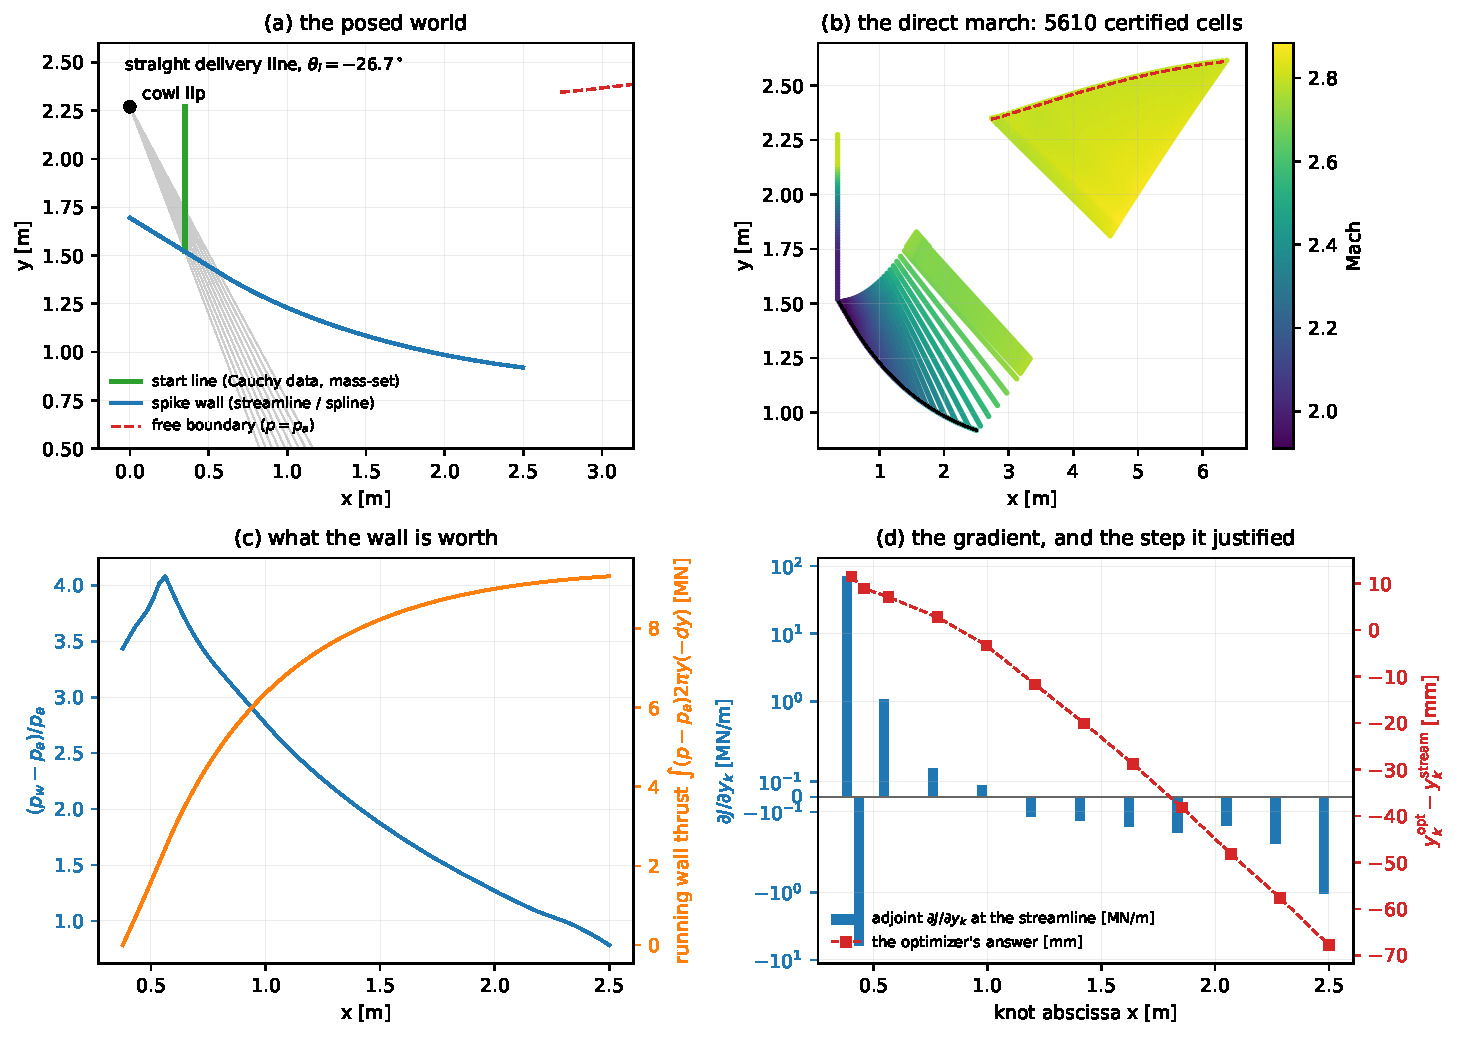
\includegraphics[width=\textwidth]{fig_worked_example.pdf}
\caption{One evaluation of the plug method, end to end, from a live
run at the working settings. (a)~The posed world: lip fan (grey
rays), the mass-set start line (green), the spike wall, and the
free boundary --- whose polyline begins where the march's first
column reaches it, one long chord downstream of the start line (the
measured first-column stride of Chapter~\ref{ch:plug}).
(b)~The direct march's mesh, one point per certified cell, coloured
by Mach: columns hug the wall, and the top rows stride into the
widening jet. (c)~Wall overpressure (left axis) against the running
wall-thrust integral (right axis): the fat end does the work, and
the flow leaves the cut still $1.8\,p_a$ above ambient.
(d)~The reverse-mode adjoint at every knot (bars, symmetric log
scale) beside the step the optimizer ultimately took (red): raise
the fat end, surrender the tail --- correct at the resolution that
computed it, and worth nothing in the limit
(Section~\ref{sec:gainresolved}). \emph{Regenerated 2026-09-16: panel~(d)'s
step is the re-adjudicated fine optimum of
Section~\ref{sec:readjudication} ($+12$ mm at the first knot, $-68$
mm at the tip), a design whose march is folded.}}
\label{fig:workedexample}
\end{figure}

\chapter{Stato, che cosa resta, e riproduzione}
\label{ch:status}

Questo capitolo è il registro. Elenca ogni suite di test che il
programma possiede e il suo verdetto, dichiara esattamente quali
grandezze un'esecuzione di progetto può fissare e quali può muovere,
dice che cosa non è ancora stato costruito e fornisce il comando che
riesegue ogni risultato da zero. Nulla qui è fisica nuova: è la parte
che serve a un lettore per verificare il resto.

\section{Stato di ogni suite}

\begin{table}[htbp]
\centering
\small
\begin{tabular}{llll}
\toprule
Passo & Carrier (\code{validation/}) & Verdetto & Capitolo \\
\midrule
Marcia del Mattone 1 & \code{a1\_ideal\_march\_jax.py} & certificata &
  (prereq.) \\
Funzionale di spinta & \code{a1\_thrust\_functional.py} & 8/8 PASS &
  \ref{ch:score} \\
Strumento di spigolo & \code{a1\_corner\_instrument.py} & 5/5 PASS &
  \ref{ch:score} \\
Driver in $\varepsilon$ vs forma chiusa & \code{a1\_driver\_eps.py} &
  4/4 PASS & \ref{ch:firstopt} \\
Marcia a parete assegnata & \code{a1\_wall\_march.py} & 5/5 + 2/2 PASS &
  \ref{ch:wallinput} \\
Verifica fra codici GENO (O3.4) & \code{g0\_geno\_crosscode.py} & PASS &
  \ref{ch:referee} \\
Moltiplicatori di Rao vs AD (O3.3) & \code{a1\_o33\_toc.py} & 9/9 PASS &
  \ref{ch:referee} \\
Strato di ciclo (collasso + RDE simulato) & \code{a1\_cycle\_layer.py} &
  5/5 + 6/6 PASS & \ref{ch:cycle} \\
Misuratore di spigolo di ciclo (voti) & \code{a1\_cycle\_corner.py} & 8/8 PASS &
  \ref{ch:cycle} \\
Cella di getto libero & \code{a1\_freejet\_unit.py} & 6/6 PASS &
  \ref{ch:plug} \\
Marcia del plug (oracolo + assi) & \code{a1\_plug\_march.py} & 6/6 + 5/5 PASS &
  \ref{ch:plug} \\
Plug troncato sotto ciclo & \code{a1\_plug\_cycle.py} & 5/5 + 9/9 PASS &
  \ref{ch:plugcycle} \\
Gemello GENO a campo intero & \code{a1\_geno\_plug\_twin.py} & 8/8 PASS &
  \ref{ch:genotwin} \\
Marcia con swirl a vortice libero & \code{a1\_swirl\_march.py} & 9/9 PASS &
  \ref{ch:swirl} \\
Ingresso generale (rotazionale) & \code{a1\_rot\_march.py} & 8/8 PASS &
  \ref{ch:generalinlet} \\
Oracolo di flusso radiale ($v<0$) & \code{a1\_source\_flow\_oracle.py} & 6/6 PASS &
  \ref{ch:compare} \\
Confronto fra configurazioni & \code{a1\_config\_compare.py} & 7/10
  (3 aperte) & \ref{ch:compare} \\
Angolo di ingresso come variabile & \code{a1\_inlet\_angle\_opt.py} & 6/6 PASS &
  \ref{ch:compare} \\
Spina a forma libera (spline + TR-SQP) & \code{a1\_plug\_spline\_opt.py} &
  7/8 (vedi sotto) & \ref{ch:spline} \\
Nodi adattivi sulla spina & \code{a1\_plug\_adaptive.py} &
  11/12 (vedi sotto) & \ref{sec:adaptive} \\
Risoluzione del guadagno (scala appaiata) & \code{a1\_plug\_gain\_resolve.py} &
  RISOLTO: guadagno $= 0$ in banda & \ref{sec:gainresolved} \\
Misuratore di campo, due vie (CFD P0) & \code{a1\_field\_meter.py} &
  3/4 (1 aperta) & \ref{sec:fmeter} \\
\bottomrule
\end{tabular}
\caption{Ogni suite certificata del Mattone~2, il suo carrier e il suo
verdetto di riferimento. ``$m/n$ PASS'' conta le verifiche della
suite, rigettatori inclusi. Due suite portano verifiche aperte anziché
assorbirle in bande allargate: le chiusure di massa e quantità di moto
del confronto fra configurazioni per il plug discendente, e l'accordo
fra le due vie del misuratore di campo. Il guadagno un tempo aperto
della spina a forma libera (il suo 7/8 e l'11/12 del carrier adattivo
registrano i verdetti delle rispettive sessioni) è ora RISOLTO dal
carrier a scala appaiata: zero entro una banda dello $0.017\%$
(\S\ref{sec:gainresolved}). Le prime due sono la stessa fisica, e la
\S\ref{sec:fmeter} affina la diagnosi precedente: la vecchia cifra era
gonfiata dal misuratore, ma un residuo vicino all'$1\%$ sopravvive su
una superficie adatta a essere integrata e sopravvive al raffinamento,
quindi è una proprietà del campo e non solo della contabilità.
\code{a1\_flux\_meter.py} non porta un verdetto proprio --- è il modulo
strumento su cui quelle verifiche vanno ricablate, non una suite.}
\label{tab:status}
\end{table}

\section{Ingressi di progetto e vincoli, a oggi}
\label{sec:designinputs}

\subsection{Che cosa un'esecuzione di progetto può fissare}

Progettare significa tenere fisse alcune grandezze e lasciare che
l'ottimizzatore muova le altre. Ogni voce qui sotto può essere tenuta
fissa in modo indipendente per un'esecuzione; ciò che non è tenuto
fisso è ciò che l'ottimizzazione è autorizzata a cambiare.

\emph{Gas e camera}: le tabelle di proprietà (qualunque modello di gas
entro il suo intervallo di validità), le condizioni di camera
$(P_0, T_0)$ --- la pressione e la temperatura che il gas avrebbe a
riposo --- e, per le esecuzioni RDE, l'intero ciclo
$P_0(\xi), T_0(\xi)$ con il peso assegnato a ciascuna fase $\xi$ del
ciclo.

\emph{Ambiente}: la pressione ambiente $p_a$ in cui l'ugello scarica,
vuoto compreso. Per un ugello a spina non è mera contabilità: entra
nel flusso stesso, poiché la frontiera di getto libero è la superficie
su cui $p = p_a$.

\emph{Geometria di gola}: il raggio di gola $y_t$ e i due raggi di
raccordo $r_{tu}, r_{td}$ che arrotondano la gola, tutte manopole
differenziabili. Tenere fisso $y_t$ \emph{è} il vincolo di portata:
una gola bloccata lascia passare una portata fissa $\dot m$, quindi
fissarne il raggio fissa la portata del motore.

\emph{Dimensione complessiva}: il rapporto di espansione $\varepsilon$
--- l'area di uscita divisa per l'area di gola, l'unico numero che
dice quanto l'ugello espande il gas (il driver a una manopola dei
Capitoli~\ref{ch:firstopt} e~\ref{ch:cycle}).

\emph{La parete}: un'uscita quando il motore genera un contorno; un
ingresso interamente assegnato nelle modalità inverse a campana e a
plug; e un'incognita parametrizzata quando viene ottimizzata --- oggi
piccole protuberanze con gli estremi bloccati, punti di controllo
spline in seguito. Bloccare l'estremo \emph{è} il vincolo di lunghezza
fissa: è esattamente il problema che Rao pose, ed esattamente ciò che
il test di stazionarietà della Sezione~\ref{sec:o33} teneva fisso.

\emph{Modalità}: piana o assialsimmetrica; un singolo punto di
funzionamento stazionario o una media di ciclo. \emph{Risoluzione}: il
numero di raggi del ventaglio, di stazioni e di righe iniziali --- non
variabili di progetto, ma fissate per ogni esecuzione e parte di ogni
banda d'errore derivata.

\subsection{Quali vincoli si possono tenere simultaneamente}

Sul lato JAX i vincoli sono oggi imposti \emph{per costruzione}
anziché da un ottimizzatore vincolato generale: la portata tenendo la
gola, la lunghezza bloccando il labbro, l'ambiente come dato posto ---
e l'ottimizzatore muove ciò che resta (oggi $\varepsilon$, o la parete
attraverso la sua base di protuberanze). Tenere più vincoli non
lineari insieme contro il gradiente AD richiede la macchina generale:
un driver SQP a regione di fiducia --- un ottimizzatore vincolato
standard che a ogni iterazione compie un passo di dimensione limitata
e impone i vincoli al primo ordine --- che è nella lista del lavoro
restante, e per il quale sono stati costruiti i percorsi certificati a
parete assegnata.

Sul lato GENO il modulo RaoPlug (il suo caso di tipo 8) accetta, dalla
sessione a due vincoli, esattamente \emph{due} vincoli simultanei. Il
primo è il \emph{vincolo di massa}, sempre attivo: la curva di
progetto è terminata dove la massa accumulata al suo interno eguaglia
il bersaglio della gola $p_c\,\pi y_t^2/c^{*}$, e quella condizione è
consumata dal punto $D$ in cui la spina viene tagliata. Il secondo è
\emph{un} vincolo di progetto a scelta dell'utente, consumato da una
bisezione sull'angolo di uscita $\theta_E$ --- rapporto di espansione,
lunghezza del plug, angolo di uscita, spinta, numero di Mach di
uscita, pressione ambiente al labbro o pressione di base $p_b$
(confrontata con il valore che la condizione di spigolo implica al
taglio fissato dalla massa, l'accoppiamento sensato con il vincolo di
massa).

Due non è un limite implementativo ma \emph{teorico}. La famiglia di
spine di Rao ha esattamente due gradi di libertà a raggio di labbro
fissato --- l'angolo di uscita $\theta_E$ e il punto di taglio $D$ ---
quindi due condizioni la esauriscono, e una terza sarebbe
sovradeterminata. L'unica via onesta a un terzo vincolo simultaneo è
liberare il raggio di labbro $y_E$ come grado di libertà di scala, una
bisezione esterna già abbozzata nelle note di progetto di GENO e non
ancora costruita.

\section{Che cosa resta, in ordine}

Il filone GENO è ora chiuso da capo a fondo. La decisione del
proprietario era di risolvere il problema a due vincoli, e la sessione
GENO l'ha centrata: la curva di progetto termina alla massa di gola
assegnata, il punto di taglio fornisce il secondo grado di libertà con
la condizione di spigolo che restituisce la pressione di base che ne
consegue, quattro difetti di rigore sono stati corretti lungo la
strada e tre verifiche indipendenti PASSANO (la dualità fra i due modi
di scrivere la condizione terminale, $2\times10^{-5}$; il limite piano
esatto, bit per bit; un'integrazione Python indipendente della curva
di progetto, tre-quattro cifre). Una voce non si è chiusa: i numeri
tabulati nell'articolo del 1961 sulla spina, così come il registro li
cita, si sono rivelati non verificabili e internamente incoerenti (la
N-74 di GENO), quindi il proprietario deve procurare l'articolo
originale. Il confronto a campo intero --- la nostra marcia del plug
eseguita sulla spina propria di GENO --- è ora certificato 8/8 nel
Capitolo~\ref{ch:genotwin}, con la differenza misurata di
tre-quattro cifre fra i due codici caratterizzata e la sua causa
depositata come questione aperta dal lato GENO
(Sezione~\ref{sec:twingap}).

L'estensione allo swirl a vortice libero è certificata a livello di
marcia nel Capitolo~\ref{ch:swirl}: la garanzia strutturale misurata
anziché assunta, una soluzione esatta di condotto riprodotta e la
regressione a swirl spento a $10^{-13}$. Usarla dentro gli studi di
plug e di ciclo è ormai una scelta di posizione del problema, non
macchina nuova. Oltre il vortice libero il flusso è rotazionale ---
e il Capitolo~\ref{ch:generalinlet} porta ora quel caso dentro la
marcia, con gli invarianti di linea di corrente trasportati e
l'ingresso $(p, T, M, \theta)$ esattamente determinato.

La parete a forma libera, elencata qui per parecchie sessioni come
l'ultimo pezzo mancante, è ora costruita: il Capitolo~\ref{ch:spline}
dà alla spina una base di spline cubiche, un gradiente aggiunto e un
driver a regione di fiducia, e il risultato è un contorno che il
programma calcola anziché ereditare. Da come è stato costruito
seguono due cose. Usa direttamente le routine spline
dell'ottimizzatore a \emph{campana} anziché una base propria, quindi
campana e plug portano ora la stessa libertà di forma e il confronto
del Capitolo~\ref{ch:compare} diventa un confronto a pari condizioni.
E la scala di rappresentazione della Sezione~\ref{sec:reprladder}
mostra l'errore del plug concentrarsi nell'unica regione in cui il suo
contorno si piega, il che è un argomento a favore del posizionamento
adattivo dei nodi anziché di un maggior numero di nodi.

\begin{enumerate}[itemsep=2pt]
\item \textbf{Risolvere il guadagno della spina a forma libera} ---
  RISOLTO (\S\ref{sec:gainresolved}): su una scala appaiata a sei
  pioli fino a $(1921,1601)$, con l'incumbente riottimizzato a
  $(121,101)$ e il modello costretto a prevedere l'ultimo piolo prima
  di vederlo, il limite del guadagno è
  $-0.011\% \pm 0.017\%$ --- zero entro la banda. La linea di corrente
  troncata è ottimale a questa lunghezza e a questa ripartizione di
  ingresso entro lo $0.028\%$; ogni guadagno misurato in precedenza
  era strumento.
\item \textbf{Posizionamento adattivo dei nodi} sulla spina --- FATTO
  (\S\ref{sec:adaptive}); la sua verifica di verdetto è la voce
  precedente, ora chiusa.
\item \textbf{Rieseguire il confronto fra configurazioni} con
  entrambi i lati a forma libera, ora che il plug ha una base --- e
  solo una volta sistemata la voce precedente, poiché un margine
  citato contro un guadagno irrisolto ne erediterebbe il problema.
\item \textbf{Il confronto con Rao a piena espansione}: porre la
  costruzione classica e questo ottimizzatore alla STESSA lunghezza
  ($5.825$ m) con massa E ambiente adattati (\S\ref{sec:vsrao}). A
  $2.5$ m i due codici descrivono macchine diverse e le loro spinte
  non sono confrontabili.
\item \textbf{Il residuo di quantità di moto dell'$1\%$ del plug}
  (\S\ref{sec:fmeter}): ora misurato su una buona superficie e
  sopravvissuto al raffinamento, quindi è la questione fisica in
  sospeso di questo ramo.
\item \textbf{La superficie di controllo nel banco O3.3}: la nostra
  caratteristica terminale è presa come un'intera colonna di griglia,
  selezionata minimizzando proprio la dispersione che la verifica poi
  riporta. La dispersione misurata ($4.0\times10^{-3}$) non mostra
  patologie, ma il luogo va fissato \emph{a priori} e fermato al
  confine del nucleo anziché scelto dalla statistica che alimenta.
\item \textbf{Ingresso da ciclo misurato}: uno scambio di dati ---
  attenzione al rigettatore di intervallo di tabella del
  Capitolo~\ref{ch:cycle}.
\end{enumerate}

\section{Su quale solutore poggiano questi numeri}
\label{sec:rebase}

Ogni risultato di questo documento è stato prodotto originariamente su
una versione del solutore di flusso sottostante, ed è stato poi
rieseguito su un'altra. L'anello di Newton del solutore è stato
cambiato in modo indipendente: dove un tempo compiva un numero fisso
di iterazioni per cella, ora si ferma quando il passo scende sotto il
limite di certificazione della cella stessa. È un cambiamento reale al
modo in cui l'aritmetica termina, e sta sotto ogni numero qui, quindi
non è stato assunto innocuo.

È stato invece misurato. Rieseguire su entrambe le versioni il caso
che fissa la base comune dà una portata concorde \emph{bit per bit}, e
spinta, Mach di uscita, velocità di uscita, pressione di uscita e
raggio di labbro concordi fra $10^{-15}$ e $10^{-13}$ relativi ---
precisione di macchina, su quattro rapporti di espansione.
L'interpretazione è immediata: l'anello a iterazioni fisse stava già
convergendo oltre il punto in cui la nuova regola di arresto si ferma,
quindi i due concordano fino all'ultima cifra che ciascuno può
portare.

Nessun numero di questo documento si muove di conseguenza. Ogni suite
elencata nella Tabella~\ref{tab:status} è stata rieseguita sul nuovo
solutore e ha restituito il proprio verdetto registrato.

\section{Riproduzione}

Ogni carrier è autosufficiente e stampa il proprio verdetto; le
esecuzioni sono memorizzate dove indicato, quindi le riesecuzioni
costano poco. Sull'host \code{s2}:

\begin{lstlisting}
cd RDE_Design-rde-nozzle-program
.venv-a1/bin/python validation/a1_ideal_march_jax.py    # Mattone 1
.venv-a1/bin/python validation/a1_thrust_functional.py  # punteggio e bussola
.venv-a1/bin/python validation/a1_corner_instrument.py  # punteggio e bussola
.venv-a1/bin/python validation/a1_driver_eps.py         # prima ottimizzazione
.venv-a1/bin/python validation/a1_wall_march.py         # la parete come ingresso
.venv-a1/bin/python validation/g0_geno_crosscode.py     # l'arbitro
.venv-a1/bin/python validation/a1_o33_toc.py            # l'arbitro
.venv-a1/bin/python validation/a1_cycle_layer.py        # lo strato di ciclo
.venv-a1/bin/python validation/a1_cycle_corner.py       # lo strato di ciclo
.venv-a1/bin/python validation/a1_freejet_unit.py       # marcia del plug (cella)
.venv-a1/bin/python validation/a1_plug_march.py         # marcia del plug
.venv-a1/bin/python validation/a1_plug_cycle.py         # plug troncato + ciclo
.venv-a1/bin/python validation/a1_geno_plug_twin.py     # gemello plug GENO
.venv-a1/bin/python validation/a1_swirl_march.py        # swirl a vortice libero
.venv-a1/bin/python validation/a1_rot_march.py          # ingresso generale
.venv-a1/bin/python validation/a1_source_flow_oracle.py # oracolo radiale
.venv-a1/bin/python validation/a1_config_compare.py     # configurazioni
.venv-a1/bin/python validation/a1_inlet_angle_opt.py    # angolo di ingresso
.venv-a1/bin/python validation/a1_plug_spline_opt.py    # spina a forma libera
.venv-a1/bin/python validation/a1_plug_adaptive.py      # nodi adattivi
.venv-a1/bin/python validation/a1_plug_gain_resolve.py  # risoluzione del guadagno
.venv-a1/bin/python validation/a1_field_meter.py        # misuratore di campo (CFD P0)
\end{lstlisting}

Due di questi hanno bisogno di dati che gli script non generano da
sé. Il gemello del plug GENO legge un campo memorizzato dal codice
Fortran indipendente (\code{validation/\_geno\_twin/}), e il banco
O3.3 legge un contorno progettato dalla stessa fonte. Entrambi sono
prodotti di un codice che questo documento non modifica, quindi sono
ingressi anziché risultati. Il banco O3.3 porta anche un secondo
stadio che l'invocazione predefinita non esegue:

\begin{lstlisting}
STAGE=stationarity .venv-a1/bin/python validation/a1_o33_toc.py
\end{lstlisting}

Questo documento stesso è costruito da
\code{docs/brick2\_doc\_src/}: \code{make\_figures.py} rigenera le
figure di dati a partire dai dati di esecuzione memorizzati, e
\code{build.sh} compila \code{main.tex} (motore Tectonic) e installa
il PDF come \code{docs/rde\_nozzle\_A1\_brick2\_thrust.pdf}.

\section{Il misuratore di campo, e il primo cancello del programma
CFD}
\label{sec:fmeter}

\code{a1\_field\_meter.py} calcola la spinta per due vie indipendenti
su qualunque campo assialsimmetrico: come integrale di pressione
sull'hardware (il flusso di quantità di moto all'ingresso più
l'integrale di parete) e come flusso di quantità di moto attraverso un
taglio verticale a valle. Non condividono né superficie, né quadratura,
né integrando, quindi la loro differenza è una misura di conservazione
anziché di contabilità.

Esiste per due ragioni che si rivelano una sola. Le verifiche non
chiuse del confronto fra configurazioni avevano bisogno di un
misuratore adatto a essere integrato. E la controparte CFD di questo
programma (\code{docs/rde\_nozzle\_CFD\_plan.md}) ha bisogno del
proprio primo cancello: un obiettivo valutabile su un campo CFD e su
un campo di marcia che sia lo \emph{stesso funzionale}, in un solo
gauge e con un solo stato di riferimento. Confrontare una spinta CFD
con una spinta di marcia calcolata diversamente riprodurrebbe, a scala
molto maggiore, l'errore che questo documento ha ormai incontrato tre
volte.

Verdetto $3/4$. La via del flusso è indipendente dalla superficie
attraverso cui è presa ($0.40\%$ su quattro stazioni); il misuratore
riproduce la spinta registrata per lo stesso caso a
$1.0\times10^{-4}$; e un rigettatore conferma che due vie calcolate in
\emph{gauge ambiente diversi} non concordano, separando di
$5.8\times$.

La verifica che non passa è l'accordo fra le due vie stesso:
$0.99\%$, contro una banda dello $0.09\%$ che il raffinamento della
marcia sostiene, e la differenza si muove appena sotto raffinamento
($0.99\% \to 0.97\%$). È dunque una proprietà del campo. Questo affina
anziché contraddire il Capitolo~\ref{ch:compare}: l'$1.49\%$ di quel
capitolo era misurato sull'ultima colonna della marcia ed era gonfiato
da essa, ma circa l'$1\%$ è reale e resta la questione fisica in
sospeso del ramo del plug.


\appendix
\chapter{I problemi incontrati, e come sono stati risolti}
\label{ch:appendix}

Un documento di riferimento che mostrasse soltanto la versione
funzionante nasconderebbe la propria prova migliore. Ogni test di
questo programma è costruito per poter dire \emph{no}: la sua banda
di superamento è derivata dall'errore misurato dello schema stesso
anziché scelta a mano, e ogni suite impianta corruzioni deliberate
--- i \emph{rigettatori} --- che devono farla fallire. Un difetto
colto dalla suite non è quindi un imbarazzo ma una misura: la prova
che lo strumento ha i denti, e un resoconto di che cosa fa la fisica
quando la si sbaglia. I capitoli principali mostrano ciascun passo
così come funziona oggi; questa appendice raccoglie, passo per passo,
che cosa è andato storto lungo la strada, come è stato diagnosticato
e che cosa è stato cambiato. Nulla qui è aneddoto --- ogni voce è
stata colta da un test e chiusa da una correzione misurata.

\section{Passo 1: la superficie di controllo non chiusa}
\label{app:sliver}

La spinta è calcolata come bilancio su una \emph{superficie di
controllo}: una superficie chiusa immaginaria tracciata attorno al
flusso, sulla quale si sommano la quantità di moto che la attraversa
e la pressione che vi spinge. Una verifica di quella contabilità è il
\emph{test di gauge} --- si somma ovunque la stessa costante alla
pressione e nulla deve cambiare, perché una costante integra a zero
su una superficie genuinamente chiusa. Fallì alla primissima
esecuzione (Capitolo~\ref{ch:score}).

Causa: l'integrale di parete della via 2 partiva dal primo
\emph{punto} di parete della maglia, lasciando scoperta una scheggia
microscopica di parete fra il labbro della gola e quel punto. La
superficie non era chiusa, quindi una costante non integrava più a
zero (il cerchio rosso nella Figura~\ref{fig:tworoutes}). Correzione:
chiudere la superficie al labbro della gola. Il residuo di quantità
di moto $R_{\rm mom}$ --- il disaccordo fra le due vie indipendenti
di calcolo della spinta --- si è \emph{stretto} una volta che la
scheggia ha smesso di nascondersi al suo interno: il difetto ne stava
assorbendo una parte del bilancio meccanico.

\section{Passo 6: il rigettatore corretto dalla fisica}
\label{app:f2rejector}

Un rigettatore è utile solo se il caso corrotto che pone è uno che il
test potrebbe plausibilmente far fallire. Il primo controllo negativo
per il test del primo integrale della Sezione~\ref{sec:o33} --- la
verifica che una particolare combinazione $f_2$ di velocità e angolo
sia costante lungo l'ultima caratteristica di un ugello ottimale ---
usava un taglio verticale arbitrario attraverso il campo di moto,
aspettandosi che $f_2$ vi variasse. Variava appena: gran parte della
coda regolare di un ugello è quasi piatta in $f_2$, quindi un taglio
verticale è un controllo negativo \emph{debole}. Quello netto è la
\emph{parete}, una linea di corrente lungo la quale $f_2$ sale del
$64\%$; il rigettatore è stato ricostruito su di essa. Lezione: anche
i rigettatori vanno scelti in base alla fisica, non alla comodità.

\section{Passo 4: l'increspatura delle cuspidi di tabella}
\label{app:ripple}

Lo stadio di gradiente del Capitolo~\ref{ch:wallinput} pose dapprima
il test ovvio: confrontare la derivata prodotta dalla
differenziazione automatica (AD) con una differenza finita ---
l'obiettivo ricalcolato dopo aver spostato un ingresso --- a
spostamenti via via più piccoli, aspettandosi che l'accordo
migliorasse. Fallì in un modo che nessuna dimensione di passo poteva
sanare. La differenza finita divergeva man mano che il passo scendeva
sotto la larghezza di una cella delle tabelle di proprietà del gas,
mentre il valore AD oscillava.

Diagnosi: le tabelle sono interpolate linearmente a tratti, quindi la
funzione che il codice implementa davvero ha piccole cuspidi a ogni
confine di cella di tabella, e la derivata \emph{esatta} di quella
funzione porta un'increspatura genuina alla scala delle celle di
tabella --- misurata a una deviazione standard di $44$, cioè lo
$0.010\%$ del gradiente e $1.2\times10^{-8}$ della spinta $J$
(Figura~\ref{fig:ripple}). Nessuno dei due numeri era sbagliato; era
sbagliato il \emph{test}. Un test puntuale AD-contro-differenze
finite su termodinamica tabulata è mal posto.

Il certificato onesto separa la curvatura regolare di $J$ (la fisica)
dall'increspatura (l'interpolazione) adattando una retta su una
spazzata di ampiezze di spostamento e verificando invece l'identità
dell'inviluppo che ne risulta --- il certificato che la suite ora
porta. Una prima analisi aveva anche etichettato erroneamente come
``increspatura'' una curvatura regolare del $2.25\%$; la separazione
per adattamento lineare l'ha corretta al vero $0.010\%$.
Un'interpolazione cubica delle tabelle rimuoverebbe l'increspatura
alla fonte. La stessa trappola attende qualunque solutore
differenziabile costruito su proprietà tabulate, linea dell'aggiunto
CFD compresa.

\section{Passo 7: tre trappole dello strato di ciclo}
\label{app:cycletraps}

Lo strato di ciclo (Capitolo~\ref{ch:cycle}) --- che rappresenta un
RDE con una famiglia di stati di camera stazionari, uno per ogni fase
$\xi$ del passaggio dell'onda --- ha incontrato tre trappole, ora
ciascuna presidiata da un rigettatore.

\begin{enumerate}[itemsep=2pt]
\item \textbf{Lo zero dell'entalpia.} L'entalpia non ha uno zero
  assoluto: ogni tabella fissa il proprio stato di riferimento, e solo
  le differenze sono fisiche. Costruire lo stato di camera di ciascuna
  fase in modo \emph{assoluto}, come $h_0 = h(T_0)$ letto direttamente
  dalla tabella grezza, sbagliava lo stato del $19\%$. Correzione:
  costruire gli stati di fase \emph{relativamente} al riferimento
  proprio delle tabelle
  ($h_0 = h_0^{\rm tab} + h(T_0) - h(T_s^{\rm tab})$, e allo stesso
  modo per l'entropia con il suo termine $R\ln(P_0/p_s)$). Presidio:
  raddoppiare la pressione di camera deve esattamente raddoppiare ogni
  pressione nel campo, $p(2P_0)/p(P_0) = 2$, ora verificato a
  $1.6\times10^{-15}$.
\item \textbf{Il progetto di picco cieco alla pressione.} Il primo
  tentativo di ``progettare alla fase di picco'' teneva fisso il
  numero di Mach di uscita --- il che non è affatto progettare al
  picco, perché ignora dove la pressione di uscita propria di quella
  fase eguaglierebbe l'ambiente. Correzione: il progetto di picco
  risolve $p_e(\varepsilon) = p_a$ per lo stato proprio della fase di
  picco (\code{eps\_star\_at\_pa}).
\item \textbf{Il troncamento silenzioso di tabella.} Una prima
  esecuzione dell'RDE simulato poneva una temperatura di camera di
  picco $T_0 = 4162$~K --- oltre il bordo di 3900~K delle tabelle ---
  e la routine di interpolazione \code{np.interp} \emph{tronca in
  silenzio} al bordo invece di protestare. L'esecuzione si completava,
  con la termodinamica appiattita di nascosto. Correzione: il ciclo
  simulato è stato riposto dentro la validità delle tabelle (picco
  3850~K), e un rigettatore di intervallo di tabella fa ora fallire
  qualunque fase la cui $T_0$ esca dalle tabelle --- la prima cosa da
  controllare quando viene immesso un ciclo misurato.
\end{enumerate}

\section{Passo 7 (assemblaggio): la trappola di segno del getto
libero}
\label{app:signtrap}

Sul bordo di getto libero --- la frontiera dove lo scarico incontra
l'atmosfera, sulla quale la pressione è assegnata e la posizione è
risolta --- la prima versione della cella scriveva la condizione sulla
velocità sostituendo i moduli,
$v = +\sqrt{q_{p_a}^2 - u^2}$ (Figura~\ref{fig:freejet}b). Quella
forma ammette in silenzio solo rotazioni verso l'esterno, perché la
radice quadrata non è mai negativa; un getto in \emph{compressione}
deve ruotare verso l'interno. Il rigettatore del test elementare U-3
--- un bordo in compressione posto su dati esatti --- ha colto la
radice spuria troncata. La cella è stata riformulata con l'\emph{angolo}
di rotazione $\theta_4$ come incognita, così il segno della rotazione
vive dentro l'incognita stessa ed entrambe le direzioni sono
raggiungibili --- la formulazione certificata 6/6 nel
Capitolo~\ref{ch:plug}.

\section{L'assemblaggio del plug: quattro lezioni strutturali}
\label{app:pluglessons}

La marcia del plug del Capitolo~\ref{ch:plug} ha raggiunto la propria
forma certificata attraverso quattro fallimenti strutturali misurati.
Ciascuno è stato colto dall'oracolo in forma chiusa --- una risposta
esattamente nota che la marcia deve riprodurre --- diagnosticato fino
a un meccanismo e chiuso da un cambiamento di progetto. Il progetto
presentato nel Capitolo~\ref{ch:plug} \emph{è} la somma di queste
correzioni.

\begin{figure}[htbp]
\centering
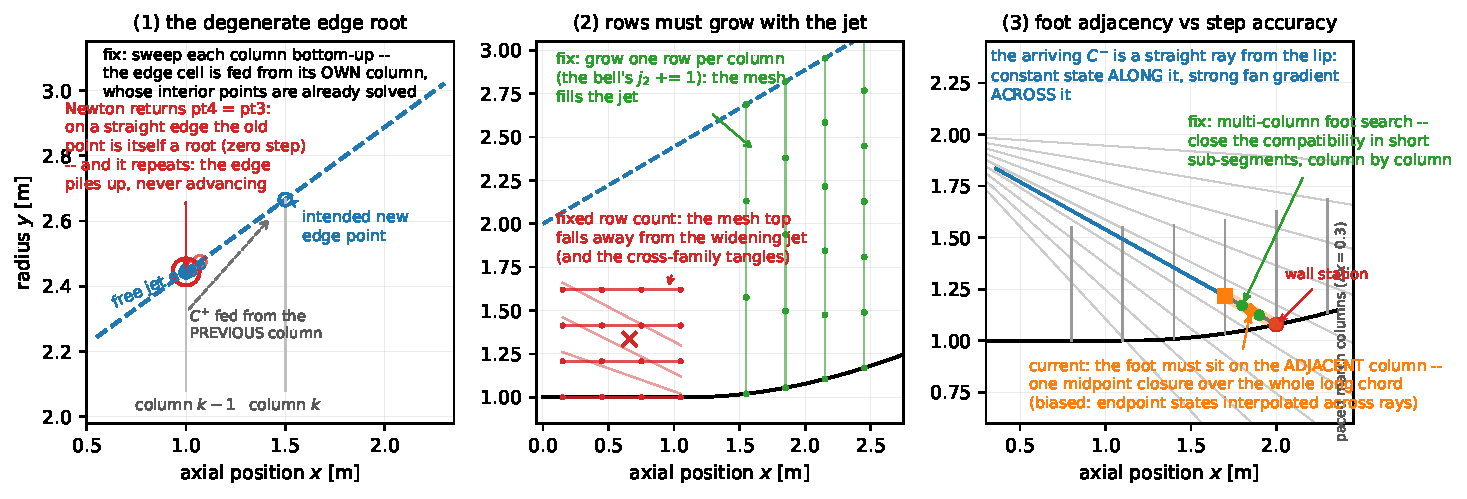
\includegraphics[width=\textwidth]{fig_plug_lessons.pdf}
\caption{Le tre lezioni misurate, disegnate nel mondo di prova
esattamente noto; tutti i pannelli hanno la coordinata assiale $x$
[m] in orizzontale contro la coordinata radiale $y$ [m] in verticale,
con la maglia che la marcia ha effettivamente costruito. (1)~La
radice degenere del bordo: i punti di bordo successivi si accumulano
in un solo luogo invece di avanzare (Sezione~\ref{app:edgeroot}).
(2)~Con un numero fisso di righe di maglia per colonna, la sommità
della maglia si stacca dal getto che si allarga (rosso); aggiungere
una riga per colonna --- lo stesso espediente che usa la marcia della
campana --- mantiene la maglia a riempire il getto (verde). (3)~La
caratteristica che arriva alla parete è un raggio rettilineo dal
labbro: lo stato è costante lungo di esso e varia fortemente
attraverso di esso. Con il piede di quel raggio forzato sulla colonna
adiacente, la relazione di compatibilità veniva chiusa da una singola
regola del punto medio su una corda lunga i cui stati agli estremi
sono interpolati \emph{attraverso} i raggi --- sistematicamente
distorta. La correzione è la ricerca multi-colonna del piede del
Capitolo~\ref{ch:plug}.}
\label{fig:pluglessons}
\end{figure}

\subsection{Lezione 1: la radice degenere del bordo}
\label{app:edgeroot}

Nel primo assemblaggio la cella di bordo libero era alimentata dalla
colonna \emph{precedente}, e nei tratti rettilinei del bordo la
risoluzione di Newton restituiva il nuovo punto esattamente sopra il
vecchio (pt4 = pt3) --- un passo nullo, ripetuto a ogni colonna: il
bordo si accumulava e non avanzava mai.

Il meccanismo (Figura~\ref{fig:edgeroot}) vale la pena enunciarlo
perché è generico. Newton non marcia, \emph{risolve}: qualunque cosa
azzeri i residui è una radice valida, compresa una inutile. In
pt4 = pt3 la condizione di linea di corrente è soddisfatta
identicamente ($0=0$), la condizione di pressione vale già (pt3 sta
sulla frontiera libera per costruzione), e la terza equazione dipende
da che cosa pt3 \emph{sia} nella maglia. Era stato creato, un passo
prima, come uscita di un segmento caratteristico lanciato dai dati di
sommità della colonna precedente --- la maglia registra letteralmente
una caratteristica che termina in pt3. Un mittente preso da quegli
stessi dati giace quindi sulla caratteristica propria di pt3
(esattamente là dove flusso e bordo sono rettilinei, poiché lì i
segmenti discreti giacciono esattamente sulle caratteristiche
rettilinee; al secondo ordine dove si incurvano --- ed è per questo
che il difetto si nascondeva finché il bordo non correva dritto), e
ritracciare quella linea non può che ritrovare la sua uscita
registrata.

La correzione: spazzare ogni colonna dal basso verso l'alto e
alimentare il bordo dal punto interno di sommità della \emph{propria}
colonna --- un punto sulla caratteristica \emph{successiva} della
famiglia, alla cui linea non si chiede affatto di colpire pt3 ma di
attraversare la \emph{linea di corrente} passante per pt3. Quella è
una linea meno inclinata, che una linea più ripida dal basso
intercetta strettamente a valle.

\begin{figure}[htbp]
\centering
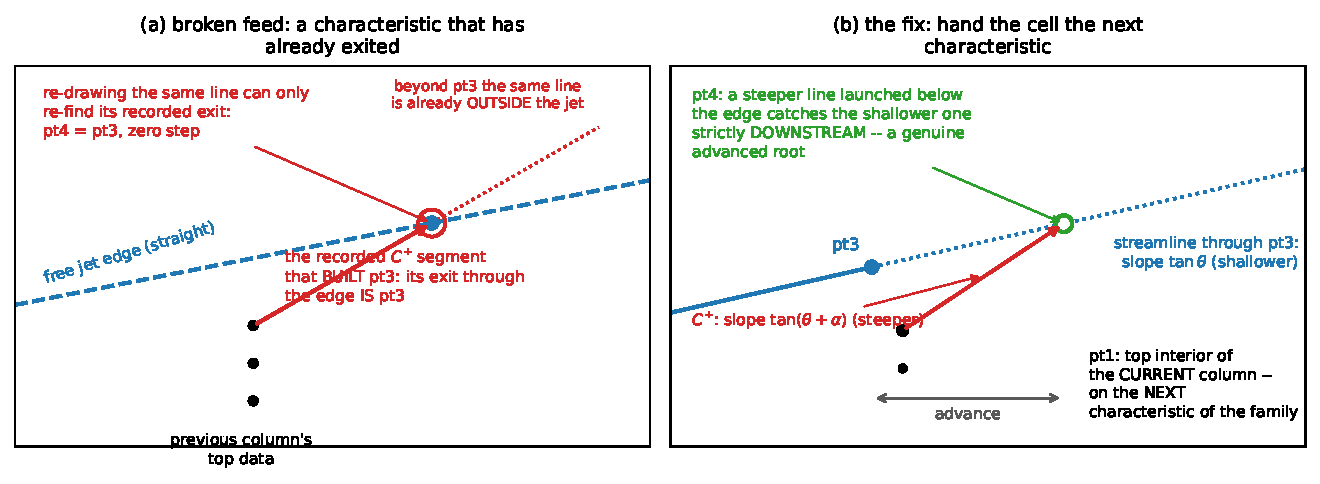
\includegraphics[width=0.95\textwidth]{fig_edge_root_geometry.pdf}
\caption{La geometria della radice degenere del bordo; entrambi i
pannelli hanno la coordinata assiale $x$ [m] contro la coordinata
radiale $y$ [m], disegnati alla scala di due celle di maglia.
(a)~L'alimentazione difettosa: pt3 esiste nella maglia solo come
uscita registrata di un segmento caratteristico dai dati di sommità
della colonna precedente, quindi un mittente preso da lì sta sulla
caratteristica propria di pt3 --- ritracciare quella linea non può
che ritrovarne l'uscita registrata, dando pt4 = pt3 e un passo nullo.
(b)~La correzione: il punto interno di sommità della colonna corrente
sta sulla caratteristica \emph{successiva}, e la sua linea deve
attraversare la \emph{linea di corrente} passante per pt3 --- un
bersaglio meno inclinato, intercettato strettamente a valle, così la
radice avanza davvero. Che cosa confrontare: l'angolo fra le due linee
in ciascun pannello.}
\label{fig:edgeroot}
\end{figure}

\subsection{Lezione 2: le righe devono crescere con il getto}

La prima maglia portava un numero fisso di righe per colonna. Ma il
getto si allarga verso valle: le caratteristiche quasi orizzontali di
una famiglia trascinavano in basso le righe fisse mentre il bordo
libero se ne allontanava salendo, finché la sommità della maglia
usciva del tutto dal getto e le due famiglie si aggrovigliavano
(Figura~\ref{fig:pluglessons}, pannello~2). La marcia della campana
sopravvive alla stessa geometria aggiungendo una riga per colonna; la
marcia del plug ora fa lo stesso in modo speculare --- il punto di
bordo libero di ogni colonna diventa una nuova riga di sommità, così
ogni colonna porta una nuova caratteristica e la maglia continua a
riempire il getto.

\subsection{Lezione 3: adiacenza del piede contro accuratezza del
passo}
\label{app:footbias}

Sistemati il bordo e le righe, la cella di parete continuava a
fallire la propria verifica di pressione a valle, e una sonda ha
\emph{nominato} il difetto: angoli di parete esatti a quattro decimali
ovunque, ma velocità di parete distorte e in deriva non appena i
segmenti si allungavano.

Il primo schema confinava il \emph{piede} della cella di parete --- il
punto sulla colonna precedente da cui la caratteristica in arrivo era
partita --- al primo segmento della colonna adiacente. Per tenere lì
il piede le colonne dovevano essere cadenzate, con la spaziatura
assiale libera di crescere fino a un limite di $0.30$. Una singola
chiusura al punto medio su una corda così lunga, che attraversa il
ventaglio di espansione, è sistematicamente distorta: la corda stessa
giace lungo un raggio rettilineo dal labbro, lungo il quale lo stato è
costante, ma i suoi stati agli estremi sono interpolati
\emph{attraverso} i raggi sulla colonna, e la regola del punto medio
propaga quell'errore trasversale sull'intero segmento lungo. I giri
intermedi (colonne allineate, crescita delle righe, cadenza) hanno
portato l'accordo di pressione di parete dal $22\%$ al $55\%$ delle
stazioni e hanno reso il fallimento riproducibile alla stessa
stazione a entrambe le risoluzioni --- la firma di un difetto
sistematico di chiusura anziché di rumore.

La correzione è la ricerca multi-colonna del piede ora nella marcia
(Capitolo~\ref{ch:plug}): le colonne sono collocate alle stazioni
fini assegnate, e la cella di parete cerca sull'intera colonna
precedente, arretrando se necessario, il segmento che racchiude la
caratteristica in arrivo. Le corde si riducono dal limite di $0.30$
alla spaziatura fra stazioni, e l'errore di una chiusura al punto
medio cala con il quadrato della corda. Quel singolo cambiamento ha
portato l'accordo di pressione di parete dal $55\%$ al $98\%$ delle
stazioni e ha riportato in banda l'angolo di bordo.

\subsection{Lezione 4: le righe fantasma, e perché un oracolo solo non
basta}
\label{app:ghostrows}

Con la ricerca del piede a posto la suite segnava ancora 3/5: ogni
cella certificata da Newton, bordo e pressione di parete in banda ---
e la conservazione della massa sbagliata del $+9\%$. La sonda ha
trovato un intero arto di maglia \emph{sotto la spina}, portatore
dello stato uniforme a monte (Figura~\ref{fig:plugbefore}).

Meccanismo: con stazioni fini, la caratteristica di una riga vicina
alla parete termina sulla parete \emph{fra} due stazioni. La marcia
prolungava comunque quella riga, e per una riga simile l'unico
incrocio che Newton riesce ancora a trovare è quello
\emph{all'indietro} --- una radice perfettamente valida delle
equazioni della cella, convergente e certificata, sul ramo sbagliato.
(La ricerca del piede stava già rilevando le terminazioni --- la sua
riga di piede saliva di una riga per colonna --- ma nulla agiva di
conseguenza.) La correzione è il \emph{consumo} delle righe del
Capitolo~\ref{ch:plug}: a una parete solida la famiglia entrante
termina, quindi le righe della colonna precedente sotto il nuovo piede
vengono ritirate e la colonna reindicizzata --- il duale esatto del
bordo che aggiunge una riga per colonna. La massa chiude poi allo
$0.026\%$.

La lezione metodologica è la ragione per cui questa appendice esiste.
Il difetto era invisibile agli oracoli puntuali (P-1, P-2) e alla
certificazione di Newton, perché ogni singola cella era stata
davvero risolta correttamente; solo il bilancio di massa
\emph{globale} lo ha visto. Le suite hanno bisogno di verifiche di
conservazione proprio perché le radici sul ramo sbagliato si
certificano localmente.

\begin{figure}[htbp]
\centering
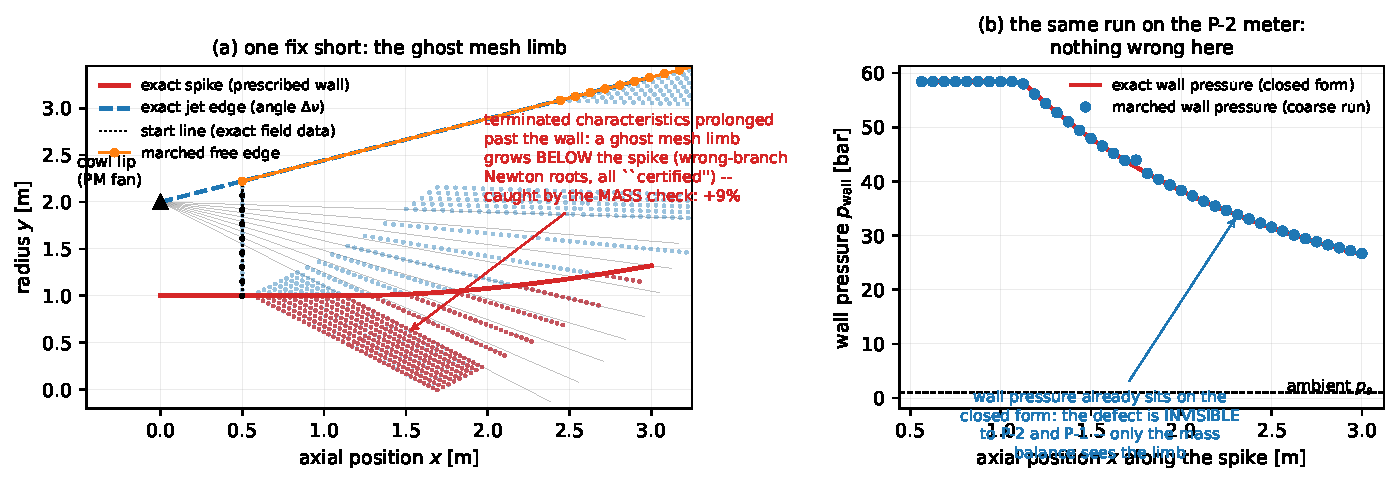
\includegraphics[width=\textwidth]{fig_plug_before.pdf}
\caption{La regressione dell'arto fantasma, riprodotta dal vivo con
l'interruttore diagnostico del carrier (\code{consume=False}).
(a)~Coordinata assiale $x$ [m] contro coordinata radiale $y$ [m]: le
caratteristiche che avrebbero dovuto terminare alla parete sono
prolungate oltre di essa e fanno crescere un arto di maglia sotto la
spina (punti rossi) --- ogni sua cella certificata da Newton, tutto
quanto sul ramo sbagliato. (b)~La stessa esecuzione misurata sulla
parete: $x$ [m] contro pressione di parete [bar], contro la risposta
in forma chiusa. Le due si sovrappongono --- ed è questo il punto: il
difetto è invisibile alle verifiche puntuali ed è stato colto solo dal
bilancio di massa, sbagliato del $+9\%$. Si confronti con lo stato
certificato, Figura~\ref{fig:plug}.}
\label{fig:plugbefore}
\end{figure}

\section{Passo 10: le lezioni di posizione del ciclo del plug}
\label{app:plugcycleposing}

Lo studio del plug troncato (Capitolo~\ref{ch:plugcycle}) ha raggiunto
la propria forma certificata attraverso tre correzioni misurate ---
due su come il problema debba essere \emph{posto}, e una in cui la
teoria stessa ha rigettato un test trapiantato a sproposito. Tutte e
tre sono disegnate nella Figura~\ref{fig:plugposing}.

\begin{figure}[htbp]
\centering
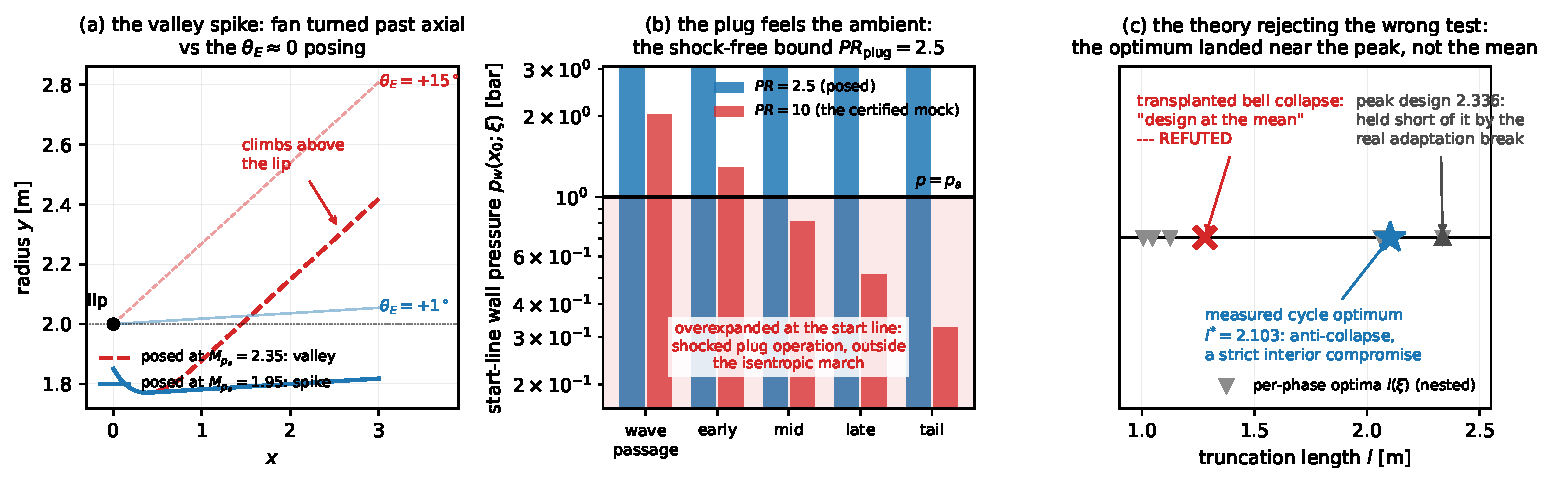
\includegraphics[width=\textwidth]{fig_plug_posing.pdf}
\caption{Le tre lezioni di posizione del passo 10, tratte dalla
macchina stessa del motore e dai numeri di riferimento.
(a)~Coordinata assiale $x$ [m] contro coordinata radiale $y$ [m]: la
spina a valle. Ponendo lo stesso ventaglio di labbro a
$M_{p_a}=2.35$ il flusso viene ruotato oltre l'assiale
($\theta_E=+15^{\circ}$) e la linea di corrente ``spina'' sale
\emph{sopra} il labbro invece di scendere; la posizione corretta
($M_{p_a}=1.95$, $\theta_E\approx0$) dà una spina genuinamente
discendente. (b)~Fase di ciclo (le cinque fasi, dal passaggio
dell'onda alla coda) contro la pressione di parete che ciascuna fase
produce alla linea iniziale [bar], con l'ambiente condiviso $p_a$
disegnato come linea. A un rapporto di pressione di camera di $2.5$
ogni fase sta \emph{sopra} l'ambiente --- sotto-espansa, e libera di
adattarsi dentro il dominio. Riscalare la stessa scaletta al ciclo
simulato certificato a $PR=10$ porta le fasi basse molto \emph{sotto}
$p_a$: un avvio con urti, che la marcia priva di urti non può
rappresentare. È quel divario a limitare il ciclo utilizzabile.
(c)~La lunghezza di troncamento $l$ [m] come retta numerica, che
segna dove cade ciascuna risposta candidata: l'aspettativa
trapiantata dalla campana (progetto alla fase media, croce rossa) è
smentita dall'ottimo di ciclo misurato $l^{*}=2.103$ --- un
compromesso interno che sta vicino al progetto di picco ma
strettamente al di qua di esso --- con gli ottimi per fase
($\triangledown$) distribuiti nell'ordine che il teorema del plug
prevede.}
\label{fig:plugposing}
\end{figure}

\subsection{La spina a valle}

Il primo mondo poneva la pressione ambiente troppo bassa (la
pressione della fase media a Mach $2.35$). Il ventaglio al labbro del
cowl ruotava allora il flusso di $+40^{\circ}$ --- oltre l'assiale ---
e la linea di corrente destinata a essere la spina si tuffava,
invertiva e saliva \emph{sopra il labbro}: una valle, non una spina,
con la parete che si avvicinava al bordo libero e ogni verifica a
valle che si rompeva sulla geometria. La correzione è la classica
condizione di progetto del plug: porre l'ambiente in modo che la
rotazione del ventaglio cancelli all'incirca l'angolo del flusso
entrante, cioè $\theta_E \approx 0$ (il flusso esce assialmente,
adattato all'ambiente), il che rende la linea di corrente
genuinamente discendente.

\subsection{Il plug sente l'ambiente: il limite di ciclo privo di
urti}

Un ugello a campana non sente mai l'ambiente: il suo flusso è
calcolato fino a un'uscita fissa qualunque sia la pressione esterna, e
$p_a$ entra solo nel punteggio. Un plug lo sente direttamente,
attraverso il bordo libero dove $p = p_a$ è imposta sul flusso
stesso.

Eseguire il ciclo simulato certificato, il cui rapporto di pressione
di camera fra la fase più forte e la più debole è $PR = 10$, contro un
unico ambiente condiviso, metteva le fasi basse $6\times$
sovra-espanse già \emph{alla linea iniziale} --- un regime con urti,
fuori da ciò che una marcia isentropica può rappresentare. Il
fallimento è stato misurato, non ipotizzato: le celle di bordo libero
esplodevano e la spazzatura scendeva riga per riga fino alla parete.
La certificazione di Newton l'ha colto, e la verifica della legge di
scala segnava una dispersione di $14.6$ dove avrebbe dovuto segnare lo
zero di macchina.

Un ciclo per uno studio di plug va dunque posto \emph{privo di urti}:
ogni fase sotto-espansa all'inizio e adattante dentro il dominio. Con
un unico ambiente condiviso questo limita il rapporto di pressione
utilizzabile --- qui $PR = 2.5$. Le affermazioni della teoria non
dipendono da $PR$, e il corpus condiziona già al flusso privo di
urti; ma il limite è un vero limite di modello che vale la pena
dichiarare, perché cicli violenti come $PR = 10$ portano le loro fasi
basse in un funzionamento del plug con urti che questo motore non sa
ancora rappresentare.

\subsection{La teoria che rigetta il test sbagliato, due volte}

Due delle verifiche della prima stesura sono fallite --- ed entrambi i
fallimenti erano la teoria che funzionava, non il codice.

Primo, la stesura trapiantava sul plug il risultato di collasso della
campana (``l'ottimo di ciclo è il progetto per la fase a pressione
media''). È fallito: l'ottimo misurato sta a $l^{*} = 2.10$ contro un
progetto alla fase media di $1.28$. È l'\emph{anti-collasso} --- il
lato opposto della dicotomia della teoria --- perché il risultato di
collasso è dimostrato solo per una parete fissa e interamente
percorsa, che un plug troncato con bordo libero non è. La verifica è
stata invertita nell'oracolo di anti-collasso ora nel
Capitolo~\ref{ch:plugcycle}.

Secondo, la stesura richiedeva che i voti per fase a $l^{*}$ --- la
pressione di parete di ciascuna fase meno l'ambiente sul piano di
troncamento --- variassero monotonamente con la fase e cambiassero
segno una volta, come certificato per la campana nel
Capitolo~\ref{ch:cycle}. Non lo fanno: su un plug le onde di
adattamento fanno oscillare la pressione di parete attorno a $p_a$,
quindi i voti puntuali campionano un'oscillazione e la fase di
passaggio dell'onda può votare negativo a una lunghezza inferiore al
proprio ottimo. La teoria afferma solo il bilancio mediato e la
struttura di compromesso, ed esattamente quelli passano; le verifiche
sovra-specificate sono state sostituite con altre fedeli al teorema
(una dispersione genuina degli ottimi per fase; $l^{*}$ come
compromesso strettamente interno).

La lezione si generalizza: un oracolo può essere trapiantato da una
classe di problemi a un'altra soltanto insieme alle ipotesi che lo
dimostrano.

\section{Passo 15: due strumenti, un vincolo}
\label{app:twoinstruments}

La spazzata sull'angolo di ingresso teneva il proprio vincolo di massa
con una ricerca di radice: spostare il raggio iniziale della spina
finché il flusso che attraversa la linea iniziale non porta la portata
di riferimento. Si valutava poi misurando quella stessa portata. Per
diverse sessioni la valutazione tornava a $7\times10^{-5}$ relativi
--- piccolo, ma un ordine sopra la banda che il raffinamento
sosteneva, quindi la verifica falliva e il fallimento resisteva alle
correzioni ovvie. Allargare la banda l'avrebbe seppellito; raffinare
la quadratura non serviva a nulla.

Il residuo non era affatto un errore. Il vincolo veniva
\emph{imposto} con una regola e \emph{valutato} con un'altra. Il
dimensionamento usava il trapezio del prodotto $\rho\, u\, 2\pi y$; il
verdetto usava il funzionale di colonna proprio della marcia, che
moltiplica medie ai punti medi, $\rho_m u_m\, 2\pi y_m$. Entrambi sono
del secondo ordine, entrambi sono corretti, e differiscono su ogni
intervallo di un quarto del prodotto degli incrementi --- che su $61$
righe è esattamente il $7\times10^{-5}$ che non voleva sparire.

Dimensionare con il funzionale che valuta lo rimuove alla fonte: il
residuo di massa scende fra $10^{-15}$ e $3\times10^{-10}$, cioè il
vincolo è soddisfatto alla precisione di macchina, e alla banda
derivata ($2.9\times10^{-4}$) non si chiede più di coprire un
disaccordo fra due strumenti.

Un secondo fallimento si è dissolto insieme a esso. Un candidato che
ruotava verso l'esterno falliva la certificazione di Newton con un
residuo peggiore di $6.5$, ed era stato letto come un limite di marcia
di quella configurazione. Non lo era: con l'anello dimensionato
correttamente, lo stesso candidato certifica a $0.05$. Un vincolo mal
imposto stava deformando in silenzio la geometria di cui poi si
incolpava la marcia.

La lezione è la forma più affilata di quella del
Capitolo~\ref{ch:compare}: non basta che un vincolo e il suo verdetto
misurino la stessa \emph{grandezza}. Devono essere lo stesso
\emph{funzionale}. Due regole corrette per uno stesso integrale
disaccorderanno al loro ordine di accuratezza comune, e quel
disaccordo si presenterà come un difetto fisico.

\section{Passo 16: tre modi di misurare male con due punti}
\label{app:twopoints}

Costruire la spina a forma libera ha prodotto lo stesso errore tre
volte in una sola sessione, in tre travestimenti. Vale la pena
enunciarlo una volta.

\emph{Primo}, la verifica che la base spline sappia rappresentare il
contorno da cui parte confrontava due conteggi di nodi e leggeva il
loro rapporto come un tasso di convergenza. Il rapporto era
$1.5\times$, troppo lento per un'interpolazione cubica, e la verifica
falliva. Ma sono presenti due errori in competizione --- uno
all'estremo destro libero della spline, uno nella stazione dove il
contorno effettivamente si piega --- e quale dei due domini si alterna
al crescere dei nodi. Due conteggi adiacenti campionano quello che
capita di vincere. Su una scala di quattro conteggi la base riduce il
proprio errore di $28\times$ ed è perfettamente adeguata.

\emph{Secondo}, il vincolo di massa era imposto con una regola di
quadratura e valutato con un'altra
(Appendice~\ref{app:twoinstruments}). Due regole corrette del secondo
ordine per lo stesso integrale disaccordano al loro ordine comune, e
quel disaccordo si presentava come un difetto fisico che nessuna
quantità di raffinamento rimuoveva.

\emph{Terzo}, l'aggiunto era valutato contro una differenza centrata
la cui banda d'errore era stimata dimezzando il passo una volta sola.
Quella stima assume che l'errore sia di troncamento. Qui non lo è: la
marcia riprodotta è solo regolare a tratti nel vettore di progetto,
quindi la differenza porta un rumore che non si riduce con il passo.
Misurata su cinque passi, la discrepanza vaga invece di calare come
$h^2$. La banda a due punti non descriveva dunque nulla, e un aggiunto
corretto veniva riportato come un fallimento.

La struttura comune è questa. \textbf{Due punti possono misurare una
differenza, ma mai un tasso, e mai l'affidabilità dello strumento che
li ha prodotti.} Ovunque questo programma valuti qualcosa contro una
banda derivata, la banda deve venire da una scala --- almeno tre
punti --- e la scala va ispezionata anziché ridotta a un singolo
rapporto. Dove la grandezza sottostante non è regolare, la scala
misura dispersione anziché troncamento, e quella dispersione \emph{è}
la banda onesta.

Vale la pena tenere anche il corollario: tutti e tre i fallimenti
indicavano il colpevole sbagliato. Nel primo si è incolpata la base,
nel secondo il flusso, nel terzo l'aggiunto. In ogni caso la colpa era
dello strumento, e in ogni caso lo strumento era la cosa che non
veniva misurata.

\section{I difetti dell'arbitro, e un binario che non si poteva
ricompilare}
\label{app:geno}

Porre la costruzione classica nel mondo di questo documento
(Sezione~\ref{sec:vsrao}) ha richiesto di eseguire il codice Fortran
indipendente a una massa e a una lunghezza che non gli erano mai state
chieste, e questo ha esposto tre difetti e un fallimento di ambiente.
Sono registrati perché due dei tre erano nostri, e perché il
fallimento di ambiente è del tipo che invalida un arbitro in
silenzio.

\emph{Un NaN dove serviva un rifiuto.} L'integratore della curva di
progetto del codice può esaurire il proprio budget di passi senza
raggiungere uno spigolo, un asse o il proprio bersaglio di massa;
questo è comportamento di base e degradava in silenzio. L'accumulatore
di massa che questo programma ha aggiunto ci passava attraverso e
restituiva una massa NaN. Un chiamante confrontava poi quel NaN con un
bersaglio ottenendo un residuo che non è né positivo né negativo, il
che avvelenava in silenzio una bisezione e alla fine affiorava come
un'entropia NaN nella termodinamica. La correzione verifica gli
incrementi \emph{prima} di accumulare --- sommare e poi sottrarre un
NaN non lo annulla --- e si ferma con una ragione distinta che il
chiamante può rigettare.

\emph{Una soluzione al problema sbagliato.} Con il presidio a posto la
bisezione sulla lunghezza girava, e restituiva un progetto che
rispettava esattamente la lunghezza mancando la massa del $63.6\%$:
aveva trovato la radice su un ramo in cui la curva si ferma al proprio
spigolo anziché al proprio bersaglio di massa. Entrambe le radici
esistono; solo una risolve il problema a due vincoli che era stato
posto. Il test di validità richiede ora la terminazione sulla massa
ogni volta che l'adattamento di massa è attivo.

\emph{Un budget scambiato per un limite.} Il tetto di $500$ passi era
vincolante su curve lunghe. Il progetto che espande fino all'ambiente
di questo documento arriva a $5.8$ m e richiede alcune migliaia di
passi; a $500$ si fermava a metà curva e riportava la lunghezza
raggiunta, ed è per questo che la spina classica per le nostre
condizioni sembrava non esistere. Alzare il tetto non può influenzare
una curva che già termina, e la riproduzione esatta del caso di
riferimento è ciò che lo dimostra.

\emph{Il binario non si poteva ricompilare.} L'eseguibile funzionante
era stato compilato con un compilatore e una libreria di algebra
lineare che non sono più installati. Ricompilare dagli stessi sorgenti
con la toolchain attuale produce un binario che \textbf{fallisce il
caso di riferimento del codice stesso} --- la spazzata sull'angolo di
uscita collassa e il numero di Mach di uscita assegnato diventa
irraggiungibile --- mentre gli stessi sorgenti a $-O0$ riproducono il
riferimento esattamente. Il codice è dunque fragile
all'ottimizzazione con il compilatore attuale, in un modo che il
precedente tollerava.

L'attribuzione conta più della correzione. Il fallimento è comparso
subito dopo le nostre modifiche, e l'inferenza ovvia era che l'avessimo
rotto noi. Ciò che ha risolto la questione è stato rimuovere del tutto
le nostre modifiche e ricompilare: il fallimento si è riprodotto
identico. Solo allora è stato legittimo dire che la colpa era del
compilatore --- e solo allora è stato sicuro tenere la correzione.

\section{Uno strumento che indovinava invece di rifiutare}
\label{app:silentclamp}

Il misuratore di campo del Capitolo~\ref{ch:status} misura massa e
quantità di moto attraverso un taglio verticale, e la sua prima
versione riportava un eccesso di massa del $6$--$7\%$ che decadeva
verso valle. La forma dell'errore era persuasiva: sembrava un difetto
di risoluzione nel campo vicino, e il sospetto ovvio --- il noto buco
di copertura della prima colonna marciata --- è stato provato per
primo. Riempire quel buco non ha cambiato nulla, a nessun
impostazione.

La causa era che il misuratore non sapeva dove fosse il getto. Una
marcia a caratteristiche emette punti di frontiera libera solo una
volta che il fronte di marcia raggiunge la frontiera, quindi la sua
poligonale di frontiera comincia a $x = 2.69$ e non esiste a monte di
lì. La routine che consulta il raggio del getto usava
un'interpolazione standard, che \emph{tronca} in silenzio fuori dal
proprio intervallo di dati e restituiva il primo valore della
poligonale come se fosse il raggio locale. Ogni taglio a monte
copriva allora una fascia esterna fantasma, e poiché l'area va come
$y^{2}$, $0.07$ m di raggio in più a $y \approx 2.3$ valgono qualche
percento della massa.

La diagnosi è stata un singolo numero: in una stazione essenzialmente
sulla linea iniziale, dove la risposta è nota per costruzione a
dodici cifre, il misuratore segnava $+6.35\%$. Uno strumento che
sbaglia dove la risposta è nota sbaglia ovunque.

La riparazione non è un'ipotesi migliore ma un rifiuto: la
consultazione ora solleva un'eccezione fuori dal proprio intervallo.
Ristretto alla finestra in cui la frontiera esiste davvero, il residuo
di massa è dello $0.6$--$1.0\%$ anziché del $7\%$. Un inviluppo
superiore della maglia è stato provato come modo di estendere la
frontiera ed è registrato qui come \emph{sbagliato}: un taglio
verticale attraverso una maglia di caratteristiche è popolato in modo
rado, quindi un massimo per stazione legge i nodi vicini alla parete e
sottostima il raggio del getto fino al $96\%$.


\begin{thebibliography}{9}
\bibitem{rao} G.~V.~R.~Rao, ``Exhaust Nozzle Contour for Optimum
Thrust,'' \emph{Jet Propulsion}, Vol.~28, No.~6, 1958. (La condizione
di spigolo, i moltiplicatori $\lambda_2,\lambda_3$ e la
caratteristica terminale come superficie di controllo.)
\bibitem{raospike} G.~V.~R.~Rao, ``Spike Nozzle Contour for Optimum
Thrust,'' \emph{Planetary and Space Science}, Vol.~4, 1961. (Il
contorno della spina ideale e il suo troncamento.)
\bibitem{zucrow} M.~J.~Zucrow e J.~D.~Hoffman, \emph{Gas Dynamics,
Volume 2: Multidimensional Flow}, Wiley, 1977. (I processi
elementari; il punto di parete inversa; la forma $(p,\theta)$ delle
equazioni di compatibilità del Capitolo~\ref{ch:generalinlet}.)
\bibitem{geno} \emph{GENO: A Method-of-Characteristics Design Code for
Supersonic Nozzles --- Theory and Implementation}, DIMA, 2026.
(\code{GENO/docs/GENO\_theory\_and\_implementation.pdf} --- l'arbitro
indipendente del Capitolo~\ref{ch:referee}, l'implementazione di
riferimento della marcia rotazionale del
Capitolo~\ref{ch:generalinlet} e il modello di formato di questo
documento.)
\bibitem{theory} \emph{RDE Nozzle Program: Theory}, questo
repository, \code{RDE\_Design\_NozzleProgram\_Theory.pdf}. (La
dicotomia di collasso, la condizione di spigolo mediata, le identità
dello swirl e il registro condizionale --- tag del corpus T3/T4, T7,
N6, C-O33.)
\end{thebibliography}

\end{document}
